\documentclass[10pt,journal,compsoc]{IEEEtran}

% Some very useful LaTeX packages include:
% (uncomment the ones you want to load)


% *** MISC UTILITY PACKAGES ***
%
%\usepackage{ifpdf}
% Heiko Oberdiek's ifpdf.sty is very useful if you need conditional
% compilation based on whether the output is pdf or dvi.
% usage:
% \ifpdf
%   % pdf code
% \else
%   % dvi code
% \fi
% The latest version of ifpdf.sty can be obtained from:
% http://www.ctan.org/tex-archive/macros/latex/contrib/oberdiek/
% Also, note that IEEEtran.cls V1.7 and later provides a builtin
% \ifCLASSINFOpdf conditional that works the same way.
% When switching from latex to pdflatex and vice-versa, the compiler may
% have to be run twice to clear warning/error messages.






% *** CITATION PACKAGES ***
%
\ifCLASSOPTIONcompsoc
  % IEEE Computer Society needs nocompress option
  % requires cite.sty v4.0 or later (November 2003)
  \usepackage[nocompress]{cite}
\else
  % normal IEEE
  \usepackage{cite}
\fi
% cite.sty was written by Donald Arseneau
% V1.6 and later of IEEEtran pre-defines the format of the cite.sty package
% \cite{} output to follow that of IEEE. Loading the cite package will
% result in citation numbers being automatically sorted and properly
% "compressed/ranged". e.g., [1], [9], [2], [7], [5], [6] without using
% cite.sty will become [1], [2], [5]--[7], [9] using cite.sty. cite.sty's
% \cite will automatically add leading space, if needed. Use cite.sty's
% noadjust option (cite.sty V3.8 and later) if you want to turn this off
% such as if a citation ever needs to be enclosed in parenthesis.
% cite.sty is already installed on most LaTeX systems. Be sure and use
% version 5.0 (2009-03-20) and later if using hyperref.sty.
% The latest version can be obtained at:
% http://www.ctan.org/tex-archive/macros/latex/contrib/cite/
% The documentation is contained in the cite.sty file itself.
%
% Note that some packages require special options to format as the Computer
% Society requires. In particular, Computer Society  papers do not use
% compressed citation ranges as is done in typical IEEE papers
% (e.g., [1]-[4]). Instead, they list every citation separately in order
% (e.g., [1], [2], [3], [4]). To get the latter we need to load the cite
% package with the nocompress option which is supported by cite.sty v4.0
% and later. Note also the use of a CLASSOPTION conditional provided by
% IEEEtran.cls V1.7 and later.





% *** GRAPHICS RELATED PACKAGES ***
%
\ifCLASSINFOpdf
    \usepackage[pdftex]{graphicx}
  % declare the path(\bm{s}) where your graphic files are
    \graphicspath{{./pics/}}
  % and their extensions so you won't have to specify these with
  % every instance of \includegraphics
  %  \DeclareGraphicsExtensions{.pdf,.jpeg,.png}
\else
  % or other class option (dvipsone, dvipdf, if not using dvips). graphicx
  % will default to the driver specified in the system graphics.cfg if no
  % driver is specified.
  % \usepackage[dvips]{graphicx}
  % declare the path(\bm{s}) where your graphic files are
  % \graphicspath{{../eps/}}
  % and their extensions so you won't have to specify these with
  % every instance of \includegraphics
  % \DeclareGraphicsExtensions{.eps}
\fi
% graphicx was written by David Carlisle and Sebastian Rahtz. It is
% required if you want graphics, photos, etc. graphicx.sty is already
% installed on most LaTeX systems. The latest version and documentation
% can be obtained at:
% http://www.ctan.org/tex-archive/macros/latex/required/graphics/
% Another good source of documentation is "Using Imported Graphics in
% LaTeX2e" by Keith Reckdahl which can be found at:
% http://www.ctan.org/tex-archive/info/epslatex/
%
% latex, and pdflatex in dvi mode, support graphics in encapsulated
% postscript (.eps) format. pdflatex in pdf mode supports graphics
% in .pdf, .jpeg, .png and .mps (metapost) formats. Users should ensure
% that all non-photo figures use a vector format (.eps, .pdf, .mps) and
% not a bitmapped formats (.jpeg, .png). IEEE frowns on bitmapped formats
% which can result in "jaggedy"/blurry rendering of lines and letters as
% well as large increases in file sizes.
%
% You can find documentation about the pdfTeX application at:
% http://www.tug.org/applications/pdftex






% *** MATH PACKAGES ***
%
\usepackage[cmex10]{amsmath}
% A popular package from the American Mathematical Society that provides
% many useful and powerful commands for dealing with mathematics. If using
% it, be sure to load this package with the cmex10 option to ensure that
% only type 1 fonts will utilized at all point sizes. Without this option,
% it is possible that some math symbols, particularly those within
% footnotes, will be rendered in bitmap form which will result in a
% document that can not be IEEE Xplore compliant!
%
% Also, note that the amsmath package sets \interdisplaylinepenalty to 10000
% thus preventing page breaks from occurring within multiline equations. Use:
\interdisplaylinepenalty=2500
% after loading amsmath to restore such page breaks as IEEEtran.cls normally
% does. amsmath.sty is already installed on most LaTeX systems. The latest
% version and documentation can be obtained at:
% http://www.ctan.org/tex-archive/macros/latex/required/amslatex/math/





% *** SPECIALIZED LIST PACKAGES ***
%
%\usepackage{algorithmic}
% algorithmic.sty was written by Peter Williams and Rogerio Brito.
% This package provides an algorithmic environment fo describing algorithms.
% You can use the algorithmic environment in-text or within a figure
% environment to provide for a floating algorithm. Do NOT use the algorithm
% floating environment provided by algorithm.sty (by the same authors) or
% algorithm2e.sty (by Christophe Fiorio) as IEEE does not use dedicated
% algorithm float types and packages that provide these will not provide
% correct IEEE style captions. The latest version and documentation of
% algorithmic.sty can be obtained at:
% http://www.ctan.org/tex-archive/macros/latex/contrib/algorithms/
% There is also a support site at:
% http://algorithms.berlios.de/index.html
% Also of interest may be the (relatively newer and more customizable)
% algorithmicx.sty package by Szasz Janos:
% http://www.ctan.org/tex-archive/macros/latex/contrib/algorithmicx/




% *** ALIGNMENT PACKAGES ***
%
\usepackage{array}
% Frank Mittelbach's and David Carlisle's array.sty patches and improves
% the standard LaTeX2e array and tabular environments to provide better
% appearance and additional user controls. As the default LaTeX2e table
% generation code is lacking to the point of almost being broken with
% respect to the quality of the end results, all users are strongly
% advised to use an enhanced (at the very least that provided by array.sty)
% set of table tools. array.sty is already installed on most systems. The
% latest version and documentation can be obtained at:
% http://www.ctan.org/tex-archive/macros/latex/required/tools/


% IEEEtran contains the IEEEeqnarray family of commands that can be used to
% generate multiline equations as well as matrices, tables, etc., of high
% quality.




% *** SUBFIGURE PACKAGES ***
\ifCLASSOPTIONcompsoc
  \usepackage[caption=false,font=footnotesize,labelfont=sf,textfont=sf]{subfig}
\else
  \usepackage[caption=false,font=footnotesize]{subfig}
\fi
% subfig.sty, written by Steven Douglas Cochran, is the modern replacement
% for subfigure.sty, the latter of which is no longer maintained and is
% incompatible with some LaTeX packages including fixltx2e. However,
% subfig.sty requires and automatically loads Axel Sommerfeldt's caption.sty
% which will override IEEEtran.cls' handling of captions and this will result
% in non-IEEE style figure/table captions. To prevent this problem, be sure
% and invoke subfig.sty's "caption=false" package option (available since
% subfig.sty version 1.3, 2005/06/28) as this is will preserve IEEEtran.cls
% handling of captions.
% Note that the Computer Society format requires a sans serif font rather
% than the serif font used in traditional IEEE formatting and thus the need
% to invoke different subfig.sty package options depending on whether
% compsoc mode has been enabled.
%
% The latest version and documentation of subfig.sty can be obtained at:
% http://www.ctan.org/tex-archive/macros/latex/contrib/subfig/




% *** FLOAT PACKAGES ***
%
\usepackage{fixltx2e}
% fixltx2e, the successor to the earlier fix2col.sty, was written by
% Frank Mittelbach and David Carlisle. This package corrects a few problems
% in the LaTeX2e kernel, the most notable of which is that in current
% LaTeX2e releases, the ordering of single and double column floats is not
% guaranteed to be preserved. Thus, an unpatched LaTeX2e can allow a
% single column figure to be placed prior to an earlier double column
% figure. The latest version and documentation can be found at:
% http://www.ctan.org/tex-archive/macros/latex/base/


%\usepackage{stfloats}
% stfloats.sty was written by Sigitas Tolusis. This package gives LaTeX2e
% the ability to do double column floats at the bottom of the page as well
% as the top. (e.g., "\begin{figure*}[!b]" is not normally possible in
% LaTeX2e). It also provides a command:
%\fnbelowfloat
% to enable the placement of footnotes below bottom floats (the standard
% LaTeX2e kernel puts them above bottom floats). This is an invasive package
% which rewrites many portions of the LaTeX2e float routines. It may not work
% with other packages that modify the LaTeX2e float routines. The latest
% version and documentation can be obtained at:
% http://www.ctan.org/tex-archive/macros/latex/contrib/sttools/
% Do not use the stfloats baselinefloat ability as IEEE does not allow
% \baselineskip to stretch. Authors submitting work to the IEEE should note
% that IEEE rarely uses double column equations and that authors should try
% to avoid such use. Do not be tempted to use the cuted.sty or midfloat.sty
% packages (also by Sigitas Tolusis) as IEEE does not format its papers in
% such ways.
% Do not attempt to use stfloats with fixltx2e as they are incompatible.
% Instead, use Morten Hogholm'a dblfloatfix which combines the features
% of both fixltx2e and stfloats:
%
% \usepackage{dblfloatfix}
% The latest version can be found at:
% http://www.ctan.org/tex-archive/macros/latex/contrib/dblfloatfix/




%\ifCLASSOPTIONcaptionsoff
%  \usepackage[nomarkers]{endfloat}
% \let\MYoriglatexcaption\caption
% \renewcommand{\caption}[2][\relax]{\MYoriglatexcaption[#2]{#2}}
%\fi
% endfloat.sty was written by James Darrell McCauley, Jeff Goldberg and
% Axel Sommerfeldt. This package may be useful when used in conjunction with
% IEEEtran.cls'  captionsoff option. Some IEEE journals/societies require that
% submissions have lists of figures/tables at the end of the paper and that
% figures/tables without any captions are placed on a page by themselves at
% the end of the document. If needed, the draftcls IEEEtran class option or
% \CLASSINPUTbaselinestretch interface can be used to increase the line
% spacing as well. Be sure and use the nomarkers option of endfloat to
% prevent endfloat from "marking" where the figures would have been placed
% in the text. The two hack lines of code above are a slight modification of
% that suggested by in the endfloat docs (section 8.4.1) to ensure that
% the full captions always appear in the list of figures/tables - even if
% the user used the short optional argument of \caption[]{}.
% IEEE papers do not typically make use of \caption[]'s optional argument,
% so this should not be an issue. A similar trick can be used to disable
% captions of packages such as subfig.sty that lack options to turn off
% the subcaptions:
% For subfig.sty:
% \let\MYorigsubfloat\subfloat
% \renewcommand{\subfloat}[2][\relax]{\MYorigsubfloat[]{#2}}
% However, the above trick will not work if both optional arguments of
% the \subfloat command are used. Furthermore, there needs to be a
% description of each subfigure *somewhere* and endfloat does not add
% subfigure captions to its list of figures. Thus, the best approach is to
% avoid the use of subfigure captions (many IEEE journals avoid them anyway)
% and instead reference/explain all the subfigures within the main caption.
% The latest version of endfloat.sty and its documentation can obtained at:
% http://www.ctan.org/tex-archive/macros/latex/contrib/endfloat/
%
% The IEEEtran \ifCLASSOPTIONcaptionsoff conditional can also be used
% later in the document, say, to conditionally put the References on a
% page by themselves.




% *** PDF, URL AND HYPERLINK PACKAGES ***
%
%\usepackage{url}
% url.sty was written by Donald Arseneau. It provides better support for
% handling and breaking URLs. url.sty is already installed on most LaTeX
% systems. The latest version and documentation can be obtained at:
% http://www.ctan.org/tex-archive/macros/latex/contrib/url/
% Basically, \url{my_url_here}.





% *** Do not adjust lengths that control margins, column widths, etc. ***
% *** Do not use packages that alter fonts (such as pslatex).         ***
% There should be no need to do such things with IEEEtran.cls V1.6 and later.
% (Unless specifically asked to do so by the journal or conference you plan
% to submit to, of course. )

\usepackage{enumitem}
%\usepackage[]{algorithm2e}
\usepackage[]{algpseudocode}
\usepackage{algorithm}
\usepackage{multirow}
\usepackage{slashbox}
\usepackage{color}
%\usepackage[numbers,sort&compress]{natbib}
%\usepackage{ulem}
%\usepackage[numbers,sort&compress]{natbib}
\renewcommand{\arraystretch}{1.3}


\usepackage{color}
\usepackage{bm}
%\usepackage{mathrsfs}
\usepackage[mathcal]{eucal}
\usepackage{amsfonts}
\usepackage{amssymb}
\usepackage{wrapfig}

\usepackage{amssymb}% http://ctan.org/pkg/amssymb
\usepackage{pifont}% http://ctan.org/pkg/pifont
\newcommand{\cmark}{\ding{51}}%
\newcommand{\xmark}{\ding{55}}%
% correct bad hyphenation here
\hyphenation{op-tical net-works semi-conduc-tor}

\newcommand{\tabincell}[2]{\begin{tabular}{@{}#1@{}}#2\end{tabular}}

\floatname{algorithm}{Algorithm}

\begin{document}
\title{Efficient and Robust Plane-Based Boolean Operations on N Meshes}
\author{%Rui~Wang,~
        %Xudong~Jiang,~
        %Hongbo~Fu,~
        %Ping~Li,~
        %Bin~Sheng~and
        %Enhua~Wu
\IEEEcompsocitemizethanks{

\IEEEcompsocthanksitem R. Wang and B. Sheng are with the Department of Computer Science and Engineering, Shanghai Jiao Tong University. Email:\{jhcz,shengbin\}@sjtu.edu.cn

\IEEEcompsocthanksitem X. Jiang is with Autodesk China Research \& Development Center. Email: xudong.jiang@autodesk.com

\IEEEcompsocthanksitem H. Fu is with the School of Creative Media, City University of Hong Kong. Email: hongbofu@cityu.edu.hk

\IEEEcompsocthanksitem P. Li is with the Department of Mathematics and Information Technology, The Hong Kong Institute of Education. Email: pli@ied.edu.hk

\IEEEcompsocthanksitem E. Wu is currently a research professor at State Key Lab. of Computer Science, Institute of Software, Chinese Academy of Sciences. Email: ehwu@umac.mo}
}

%\markboth{Journal of \LaTeX\ Class Files,~Vol.~13, No.~9, September~2014}%
%{Shell \MakeLowercase{\textit{et al.}}: Bare Demo of IEEEtran.cls for Computer Society Journals}

\IEEEtitleabstractindextext{
\begin{abstract}
  Constructive solid geometry (CSG) is widely used for computer aided design and manufacturing. However, boolean operations, which compute the boundary representation of CSG, have been suffered from robustness and efficiency problem for more than three decades. We propose a fast and exact boolean operation method which is unconditionally robust for regular set solids. We notice that among previous works,boolean methods using plane representations (P-reps) of meshes are easy to achieve robustness, but hard to be efficient. On the other hand, methods based on boundary representation (B-reps) of meshes are fast but not robust unless exact arithmetic is applied. Therefore, we choose to combine P-reps with B-reps, which allows us to take the advantages of both. Our method is globally based on B-reps for its efficiency, and P-rep geometry is applied locally to ensure robustness. Comparison experiments with state-of-the-art techniques show that our method is unconditionally exact and robust, while is competitively efficient as non-robust methods.
\end{abstract}


\begin{IEEEkeywords}
boolean operations, CSG evaluation, plane-based geometry
\end{IEEEkeywords}

}

\maketitle


\IEEEdisplaynontitleabstractindextext
\IEEEpeerreviewmaketitle

\IEEEraisesectionheading{\section{Introduction}\label{sec:introduction}}
\IEEEPARstart{C}{onstructive} solid geometry (CSG) has long been a popular modeling tool of computer-aided design and computer-aided manufacturing (CAD/CAM). It constructs complex models by combining primitives using a series of regularized boolean operations \cite{requicha1977mathematical,tilove1980closure}: union, intersection and difference. CSG can be converted into the widely-used boundary representation (B-rep) through boolean operations, which is an classical topic with history of over three decades.

In general, there are two major types of boolean algorithms according to how they deal with intersection between primitive meshes. Approximate methods \cite{wang2011approximate,pavic2010hybrid,biermann2001approximate} redicretize the intersection areas, fit vertices approximatively and rearrange topology. On the other hand, exact method do not change vertex positions, retain as many input elements  (e.g., faces, vertices and topology) as possible. In many applications, exact methods are preferred for their accuracy. Also, using exact methods, the clear mapping between the surface of input and output meshes makes it easier for the inheritance of information like face colors and materials.


However, for exact boolean operation methods, there is always a bargain between robustness and efficiency. Many exact boolean operation methods focus on efficiency. But for robustness, the solutions are either exact arithmetic \cite{barki2015exact,zhou2016mesh} or trivial workarounds to avoid degenerations, such as setting a tolerance \cite{feito2013fast,segal1990using} and rotating the primitive with small angles \cite{douze2015quickcsg}. Methods using exact arithmetic are significantly slower, and workarounds are often case dependent and not reliable. Recently, some methods \cite{bernstein2009fast,campen2010exact} seek unconditional robustness by avoiding geometry constructions (such as computing new vertex coordinates) and using only predicates. Their key idea is to utilize plane-based representations (P-reps) of meshes instead of boundary representation (B-reps), which comes from the observation of Sugihara and Iri \cite{sugihara1990solid} that boolean operations can be performed without geometry constructions if P-reps are used. While these plane-based methods are generally faster than exact arithmetic ones, they still suffer from performance issue because of the complex conversions among different representations. Also, the incoherence between different representations requires extra steps to reconstruct geometry connectivity, leading to extra computation burden and more complex topology.

Inspired by these previous work, we develop an unconditionally robust boolean operation method which is as robust as P-rep-based method and as fast as non-robust B-rep-based method. To achieve this, we embed P-rep information into faces of B-reps, forming hybrid representation of meshes. We avoid geometry constructions throughout our method, and convert all necessary computation into predicates under the hybrid representation. In general, the B-reps information is used for coarse tests and efficient face neighbor query, while P-reps information is for exact geometry computation. During intersection computation, we encode the intersections between meshes into sets of planes and use these planes to perform exact tessellation. After that, we classify each faces in the tessellated meshes using local binary space partition (BSP) trees, which also facilitate the previous plane-based representation to guarantee exactness.  In addition, while most previous boolean operations can only deal with two meshes, our method can perform boolean operations with arbitrary meshes in one call, instead of recursively doing incremental boolean operations. In this way, our method could save computation time by avoiding repetitive computation. The experiments show that our method is much faster than existing robust exact methods, while only about two times slower than the state-of-art non-robust exact methods.



\section{Related Work}

Boolean operations have been researched for over three decades since it inception in the 1980s \cite{requicha1985boolean, laidlaw1986constructive}. Previous works can be classified into two categories: exact methods and approximate methods. Exact methods retain vertex positions. Also the topology of the input meshes is preserved as much as possible. The coordinates of intersection points between input meshes are computed by input configurations to construct the topology around intersection. However, the coordinates cannot be represented exactly using fix-precision float-point numbers and the robustness is always a problem. On the other hand, approximate methods rediscretize the input mesh surfaces using techniques such as voxels, octrees and Layered Depth Images. They can reach better performance and robustness, but the loss of geometry information and precision is inevitable.

\subsection{Exact Methods}

\iffalse
\begin{figure}[t]
\centering
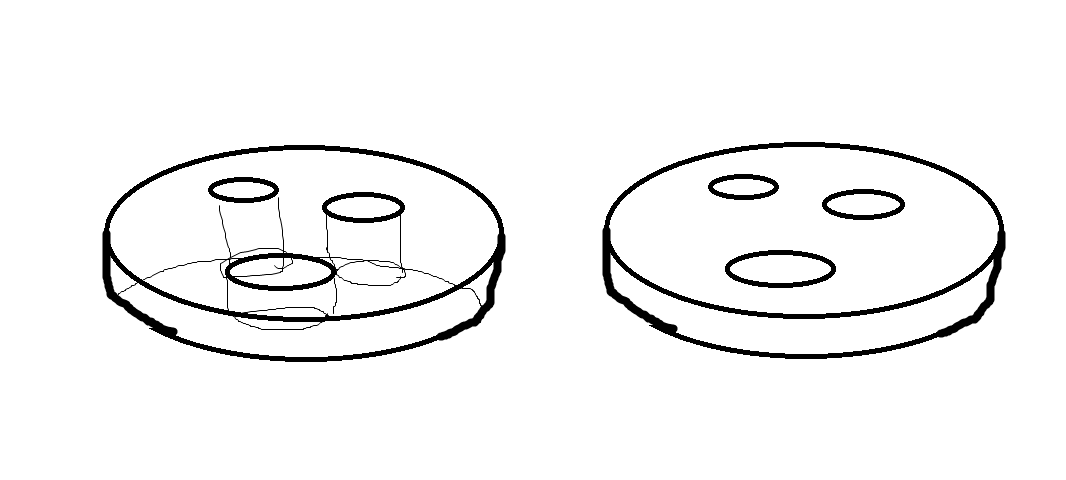
\includegraphics[width=2.5in]{coplanarexample}
\caption{{\color{red}{Sketch: the example of coplanar cases in a boolean operations with four cylinders}}}
\label{fig:coplanarexample}
\end{figure}
\fi

For exact methods, some \cite{ogayar2015deferred,douze2015quickcsg,zhou2016mesh,xu2013fast,feito2013fast} pursues efficiency but cannot guarantee robustness in degenerate cases. Most of them are implemented by fix-precision float-point arithmetic and numerical errors are inevitable. Douze et al. \cite{douze2015quickcsg} implemented very efficient method that can handle very large meshes. Also, they can perform non-incremental boolean operations: evaluating the final result mesh of CSG all at once instead of decomposing the CSG into a series of incremental boolean operations. However, their method can neither deal with coplanar cases nor guarantee accuracy of topology. In fact, large CSGs are more complex and more likely to contain degenerate cases, and more vulnerable under numerical errors. Efficiency only is far from being practical.


Many researchers have attempted to solve robustness issue for exact boolean operations using arbitrary precision arithmetic \cite{banerjee1996topologically, fortune1995polyhedral, keyser2004esolid, granados2003boolean, hachenberger2005boolean} and exact interval computation \cite{fang1993robustness, hu1996robust, segal1990using}. However, these methods are too expensive in computation time and memory to be practical for large CSGs. For example, one of the available implementation of robust exact boolean operations method is CGAL's \cite{cgal:hk-bonp3-15a} exact-arithmetic implementation \cite{granados2003boolean} of Nef polyhedra \cite{bieri1988elementary}. It requires conversions between Nef polyhedra and input mesh data structures during evaluation and is more than 50 times slower than non-robust booleans \cite{bernstein2009fast}.


\subsection{Approximative Methods}

Since efficiency, accuracy and robustness are hard to be satisfied at the same time, some method choose to sacrifice accuracy for better efficiency and robustness. Most of such methods are based on conversion to volumetric representations. However, the quality of result mesh depends on the resolution of the volume grid and better quality requires dramatically higher resolution. To accelerate this process, some try to reduce the complexity of the output mesh \cite{varadhan2004topology} and others try to preserve non-intersected areas of the input mesh to avoid redundant tessellation \cite{pavic2010hybrid,wang2011approximate,zhao2011parallel,hable2005blister,ogayar2006gpu}. Also, with the development of general-purpose computing on graphics processing units (GPGPU), many of them utilize the grand computation power of graphics hardware for boolean operations. These methods have good performance and are suitable for interactive applications. However, the fundamental problem of approximate methods is owing to grid-depend nature of volumetric calculations: they inevitably suffers from geometric detail loss and unwieldy topology changes.


\subsection{Plane-Based Methods}
\label{sec:pbrelated}

The concept of plane-based representations (P-reps) of polygonal meshes was first described by Sugihara and Iri \cite{sugihara1990solid}. P-reps provide essential benefit for boolean operations that no new geometry primitive has to be constructed to obtain the results---they can be composed of a subset of the planes from the input polyhedra. It means the computation can include only geometry predicates, which are much easier to be implemented exactly and robustly. Based on P-reps, Berstein and Fussell \cite{bernstein2009fast} combined the P-reps with binary space partition (BSP) trees \cite{thibault1987set,naylor1990merging} to develop a boolean operation method which is unconditionally robust under consistent inputs . Compared to B-rep-based methods, their method does not rely on exact arithmetics to be robust. However, the merge of two BSP trees is an $O(mn)$ time complexity process, where $m$ and $n$ are the size of the trees. It makes this method impractical for large meshes. Later, Campen and Kobbelt \cite{campen2010exact} improved their method by localize BSP operations using an octree. The mesh refinement only takes place locally near intersections, which is much faster than Berstein and Fussell's work.


\section{Background and Overview}

\label{sec:overview}
Our method is designed for boolean operations on arbitrary number of regular triangle meshes \cite{requicha1985boolean}. Input meshes are required to be free from self-intersecting, and they are represented with B-reps with geometry connectivity (e.g., halfedge, winged-edge, etc.). Despite of these requirements, our method is robust and not sensitive to topology deficiencies like holes and self-intersections and works correctly if deficiencies are not near the intersection areas between meshes.


\subsection{Boolean Numerical Errors}
\label{sec:paradigm}

The boolean operation of triangle meshes is in essence a process of face selection. Namely, given a boolean function, it reserves those primitive faces that pass the function and drop the others to generate the final mesh. Unfortunately, for B-rep meshes, not all the input faces can be classified as a whole, since for faces near the intersections, only parts of them belong to the final mesh. Therefore, we need an extra step aiming at detecting intersections between meshes and performing tessellation. Most of the boolean operation methods follow this two-step paradigm, which consists of intersection computation and face classification. So is our method.

The first step is intersection computation. Input faces are tested in pairs to compute their intersections. Each input meshes are tessellated according to the intersection results, making every face be completely inside, outside or on the boundary of other primitives. The tessellated meshes are what we called \emph{intersection-free meshes}. Unfortunately, under fix-precision float-point arithmetic, intersection tests are error-prone: first, degenerate cases of intersection are hard to detect; second, when there are intersections, new vertices are introduced into the geometry, whose coordinates cannot be exactly represented by fix-precision float-point numbers.

The second step is face classification. We evaluate whether a given face $\bm{s}$ belongs to the final geometry according to the $n$-primitive boolean function $f$ :
\begin{equation}
\lambda_f(\bm{s}) = f(\boldsymbol{\Lambda}(\bm{s})) = f(\lambda_1(\bm{s}), \lambda_2(\bm{s}), \cdots, \lambda_n(\bm{s})).
\end{equation}
The parameter $\lambda_i(\bm{s})$ is space indicator with respect to mesh $M_i$. To compute $\lambda_f(\bm{s})$ and classify $\bm{s}$, one has to know the space indicators with respect to all the primitives ($\boldsymbol{\Lambda}(\bm{s})$). A space indicator has four conditions: completely inside (\emph{in}), completely outside (\emph{out}), on the boundary with consistent normals (\emph{same}) or opposite normals (\emph{oppo}). The rules of boolean function evaluation are described in \cite{douze2015quickcsg,feito2013fast}.

\begin{figure}[t]
\centering
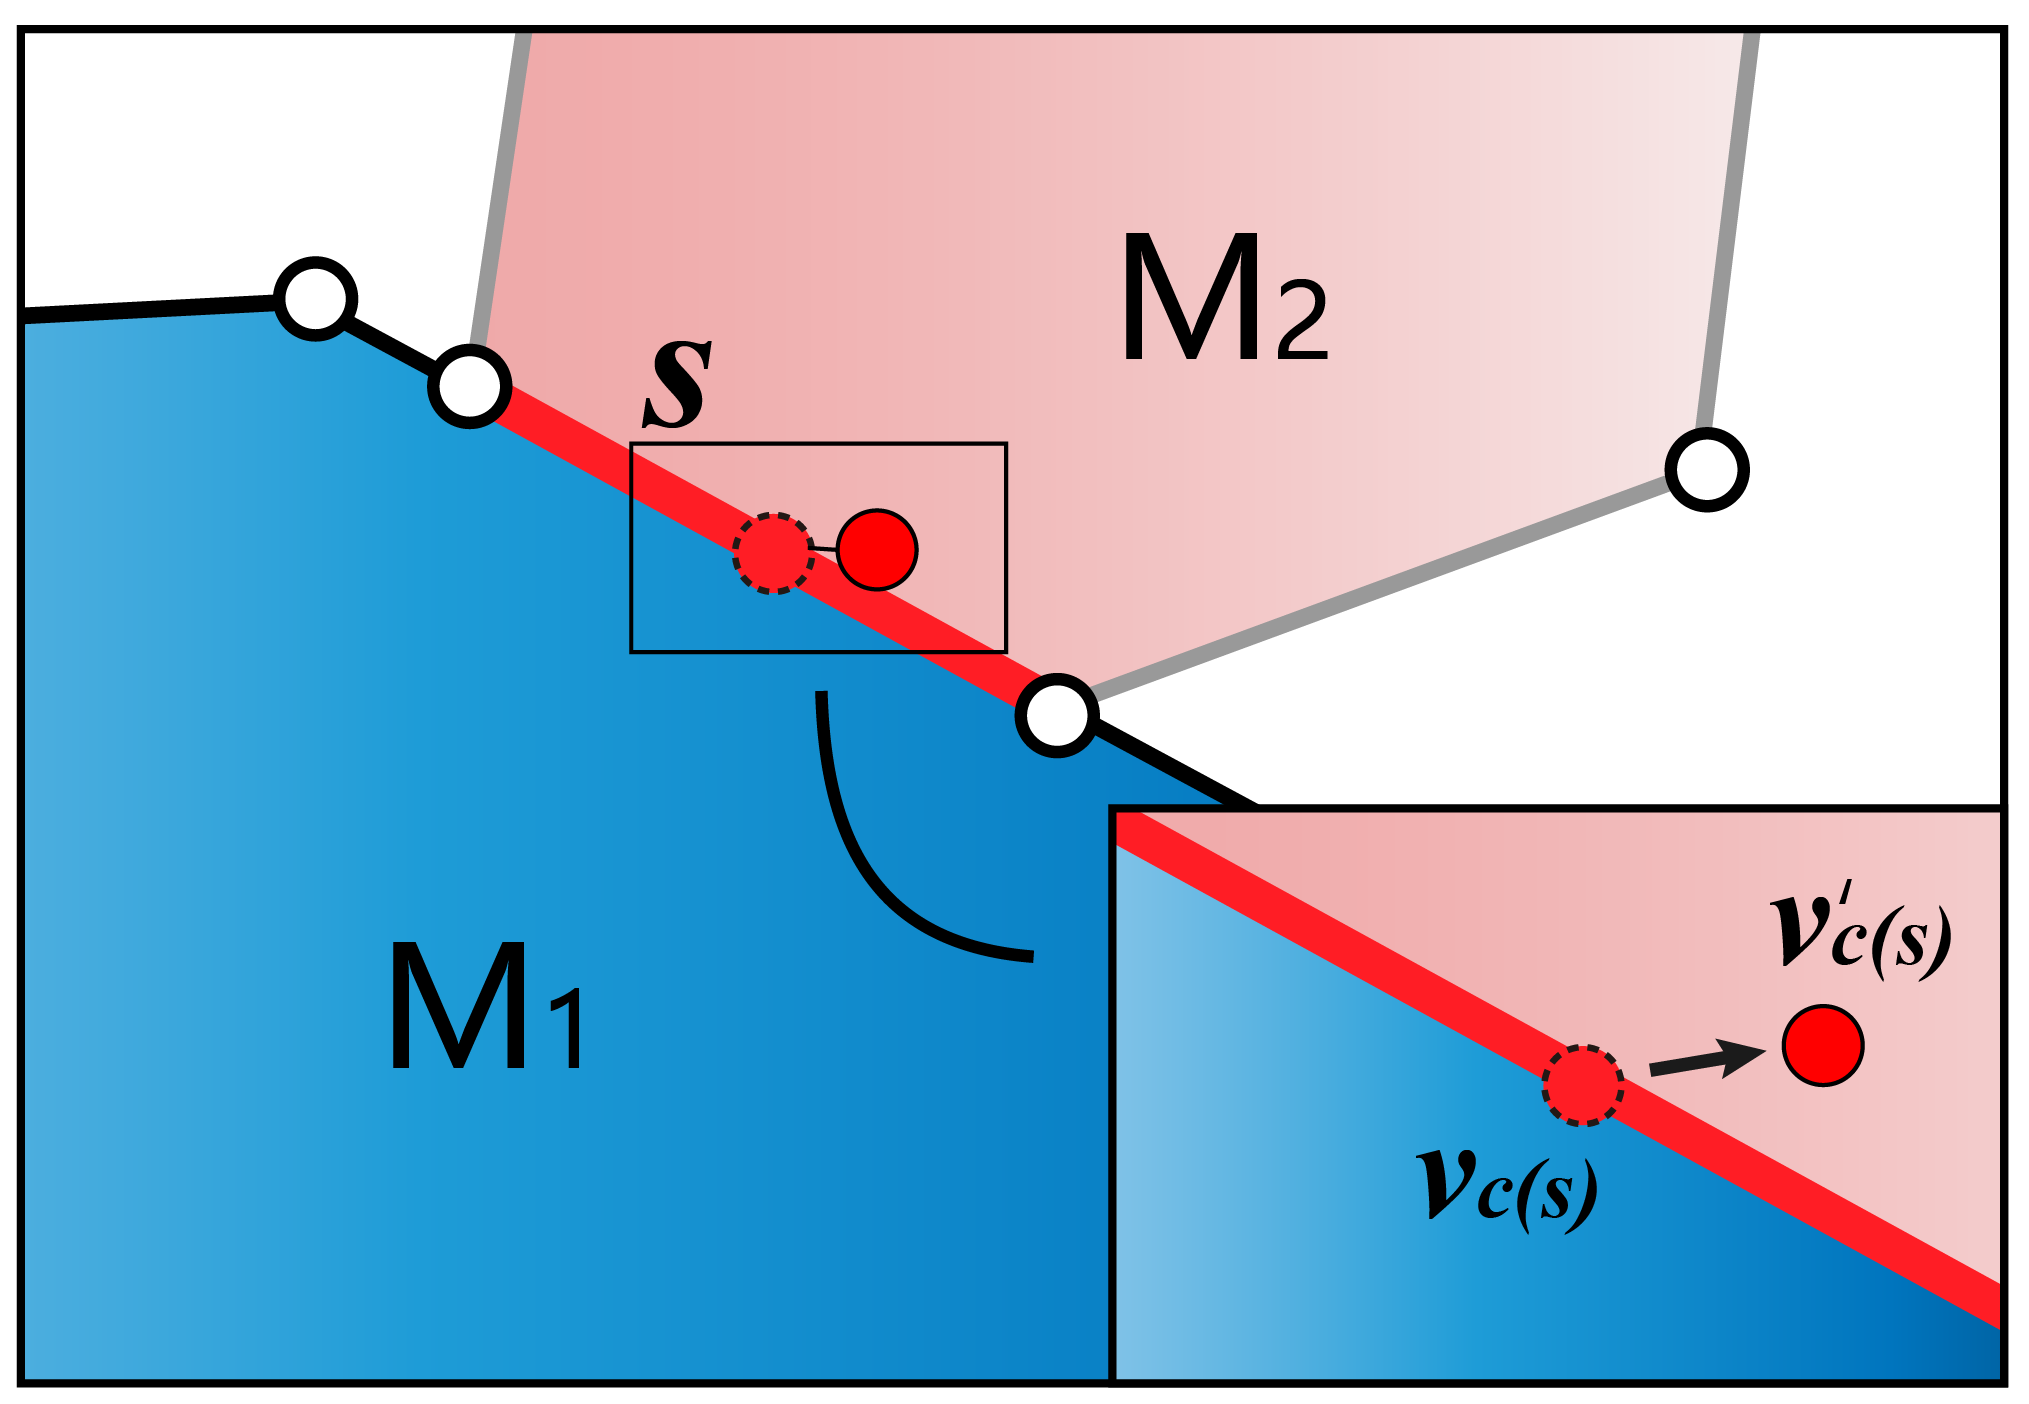
\includegraphics[width=2.2in]{boolean-01}
\caption{In the 2D view, face $\bm{s}$ (the red line segment) from mesh $M_2$ is on the surface of mesh $M_1$. However, because we use face barycenter $\bm{v}_{c(\bm{s})}$ to compute the indicator, whose coordinates contains round-off error, the point could  move to $\bm{v'}_{c(\bm{s})}$. Then we might falsely classify $\bm{s}$ as outside of $M_1$.}
\label{fig:falseclass}
\end{figure}

Face classification also suffers from numerical errors. Many methods classify face according to the indicators of its barycenter using point-in-polyhedron test \cite{feito2013fast,campen2010exact}. However, coordinates of barycenters cannot be exactly represented and could generate false classification (illustrated in Fig. \ref{fig:falseclass}). What makes the problem worse is that for the large amount of faces and input meshes, many methods \cite{pavic2010hybrid,feito2013fast,ogayar2015deferred,zhou2016mesh} take the benefits of the local coherence of indicators, classifying neighboring faces together . Despite of the performance improvement, it can propagate false classification to neighboring faces and lead to wide-range failure.


\subsection{Plane-based Geometry}

\begin{wrapfigure}{r}[0in]{0in}
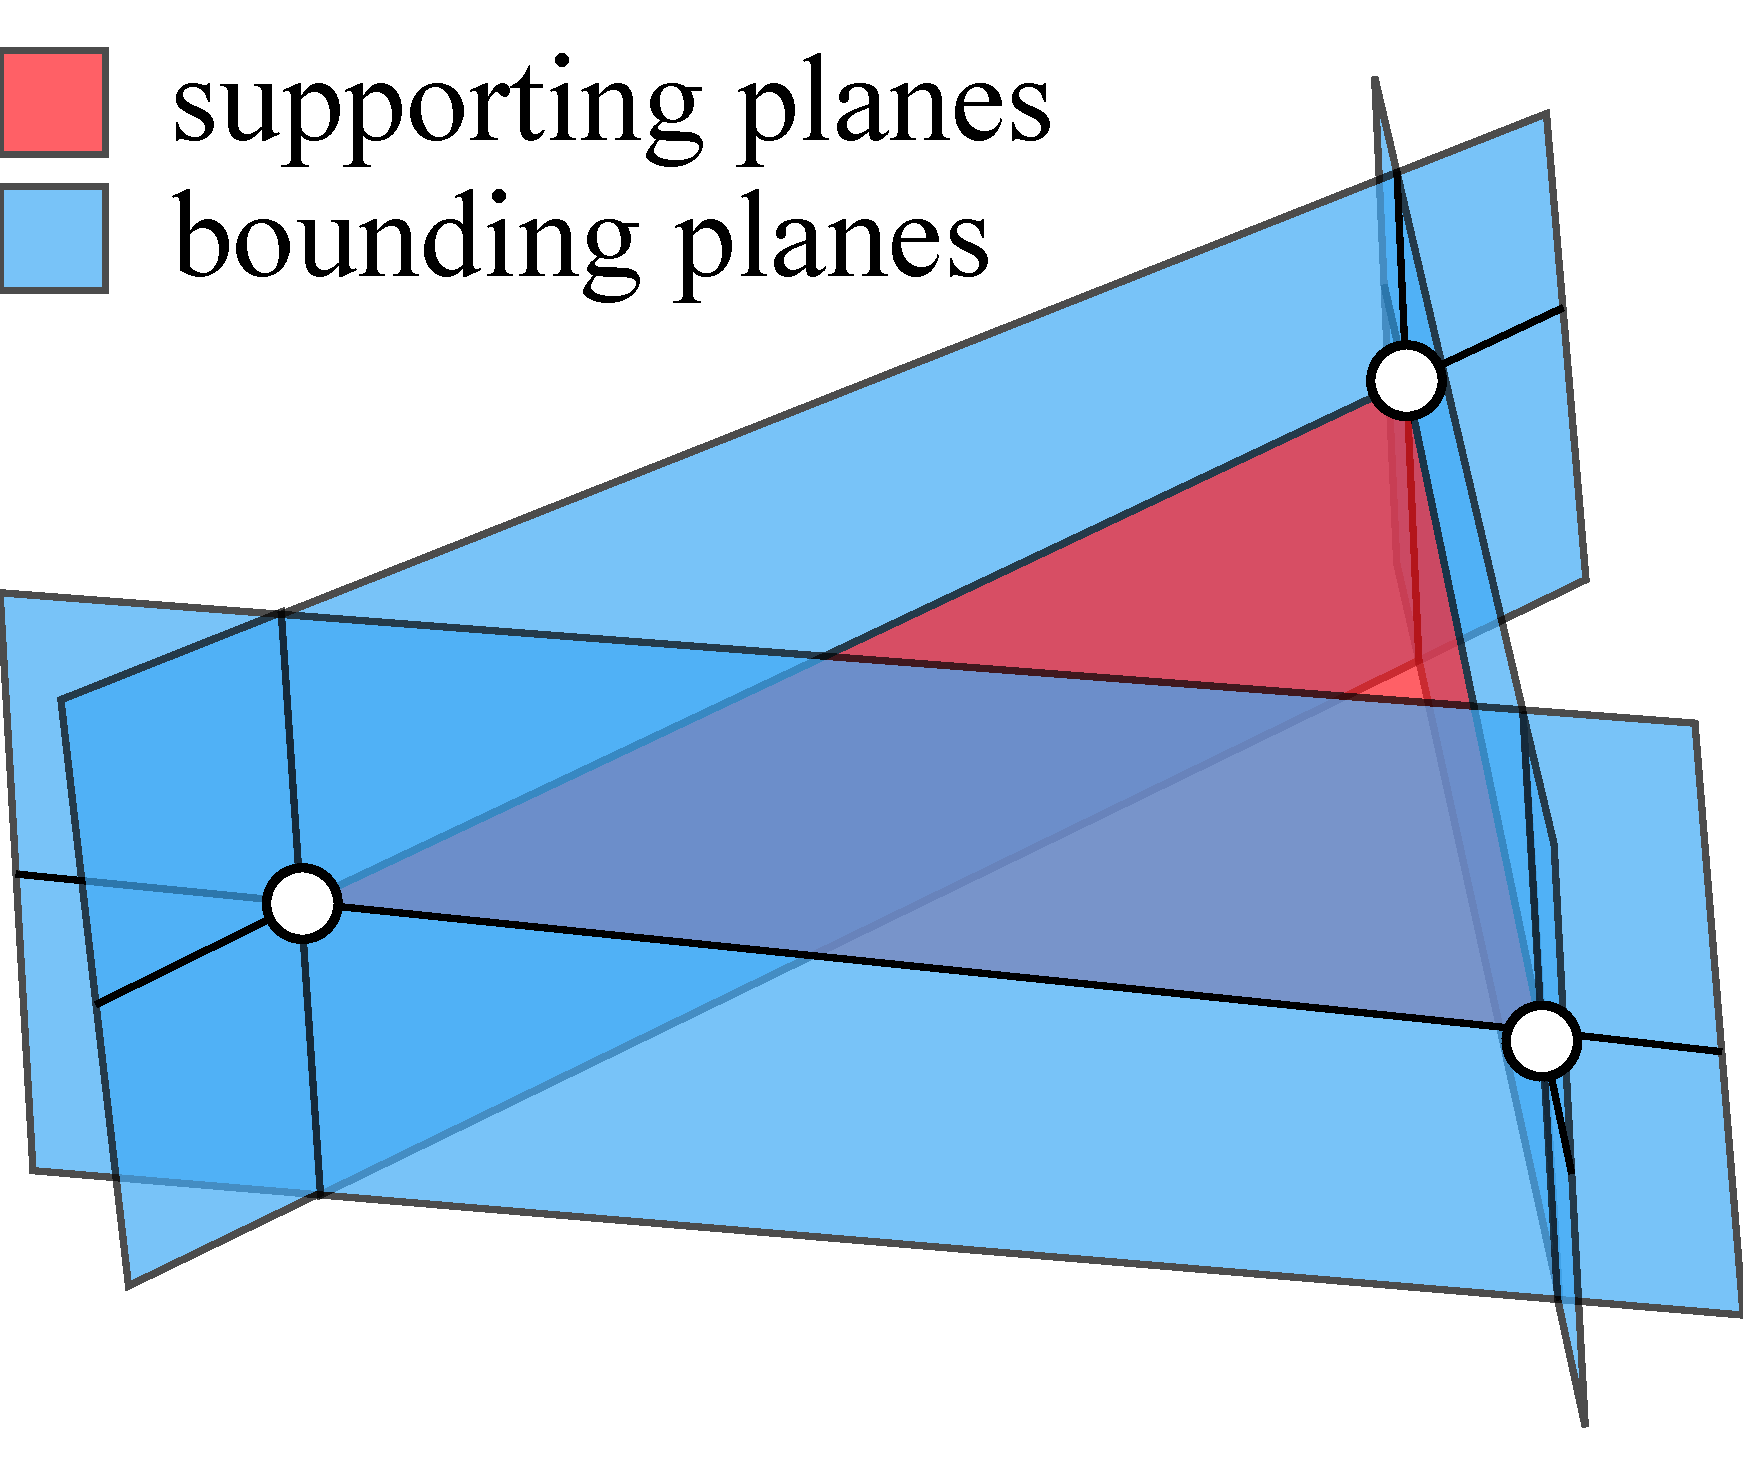
\includegraphics[width=1.5 in]{p-reps}
%\caption{Plane-based representation of triangle}
\end{wrapfigure}

In our method, we avoid numerical errors by embeding P-reps into conventional B-rep-based boolean algorithms and substituting constructions under B-reps with predicates under P-reps. Using P-reps, each face $\bm{s}$ with $n$ edges is represented by a supporting plane $\bm{p}_{s,sp}$, where the face lies, and a list bounding planes $\{\bm{p}_{s,b}^i \ \vert\  i = 0, 1,...,n-1\}$. Each edge line $\bm{e}_{\bm{s}}^i$ is represented by intersection $\bm{p}_{s,sp} \cap \bm{p}_{s,b}^i$. Corner vertex $\bm{v}_s^i$ is represented by $\bm{p}_{s,sp} \cap \bm{p}_{s,b}^i \cap \bm{p}_{s,b}^{{(i+1)}\bmod{n}}$. We use Campen et al.'s method \cite{campen2010exact} for exact conversion of triangles to their P-reps. All geometry predicates are computed using filtering techniques proposed by Shewchuk \cite{shewchuk1997adaptive} for both exactness and efficiency.


Other commonly used notations in this paper are presented here.
%A plane $\bm{p}$ can be represented by four scalar coefficients $a(\bm{p}), b(\bm{p}), c(\bm{p}), d(\bm{p})$.
The normal of a plane $\bm{p}$ is denoted as $\bm{n}(\bm{p})$. A line $\bm{l}$ can be represented by intersection of two planes $(\bm{p}_l^0 \cap \bm{p}_l^1)$, or in short, $\bm{l}\colon(\bm{p}_l^0 \cap \bm{p}_l^1)$. The positive direction of the line $\bm{l}$ is defined by $\bm{n}(\bm{p}_l^0) \times \bm{n}(\bm{p}_l^1)$. A point $\bm{v}$ can be represented by non-trivial plane triples $(\bm{p}_v^0 \cap \bm{p}_v^1 \cap \bm{p}_v^2)$, or in short, $\bm{v}\colon(\bm{p}_v^0 \cap \bm{p}_v^1 \cap \bm{p}_v^2)$.

\iffalse
Given that the input vertex coordinate has $L$-bit precision including sign, the precisions of the four plane coefficients are $L_a, L_b, L_c, L_d$, which have to satisfy the following requirements:
\begin{equation}
\begin{split}
&L_a=L_b=L_c\ge 2(K-1)+1+1,\\
&L_d\ge(L_a-1)+(L-1)+2+1.
\end{split}
\end{equation}
Here $K$ is the maximum bits required to represent edge vector components in input meshes. If we use $M$ bits to store each plane coefficient, basically $M$ has to be greater than $L_d$. In our implementation, we actually use a more strong constraint $M \ge L_d+1$. Under this constraint, given a $L$-bit vertex $\bm{v_i}$, we can compute the orientation of plane $p_j$ with respect to $\bm{v_i}$ by the sign $\bm{n}(\bm{p_j})\cdot\bm{v_i} + d(\bm{p_j})$, which requires no more than $M$ bits. It allows very fast plane orientation predicates which accelerates the early rejection in our triangle-triangle intersection tests (\S \ref{section:isect}).


Let $\delta = 2^{K-L-1}$ be the relative length (in max-norm) of the longest edge in the mesh (relative to the bounding box). If we use IEEE 754 double float point number ($M=53$) and assume $\delta \le 2^{-5.5} \approx 0.022$, the maximum input precision $L$ can reach to 20, which is enough for most application (for standard IEEE 754 single float point number, the precision is 24-bit).
\fi

\label{sec:substrates}
Plane-based geometry predicates used in our method are mostly well-discussed in previous work \cite{bernstein2009fast,banerjee1996topologically}. In the following, we focus on two predicates related to sorting, which are designed for our method particularly.

\vspace{0.5em}
\noindent \textbf{Linear ordering of points}

\begin{figure}
  \centering
  % Requires \usepackage{graphicx}
  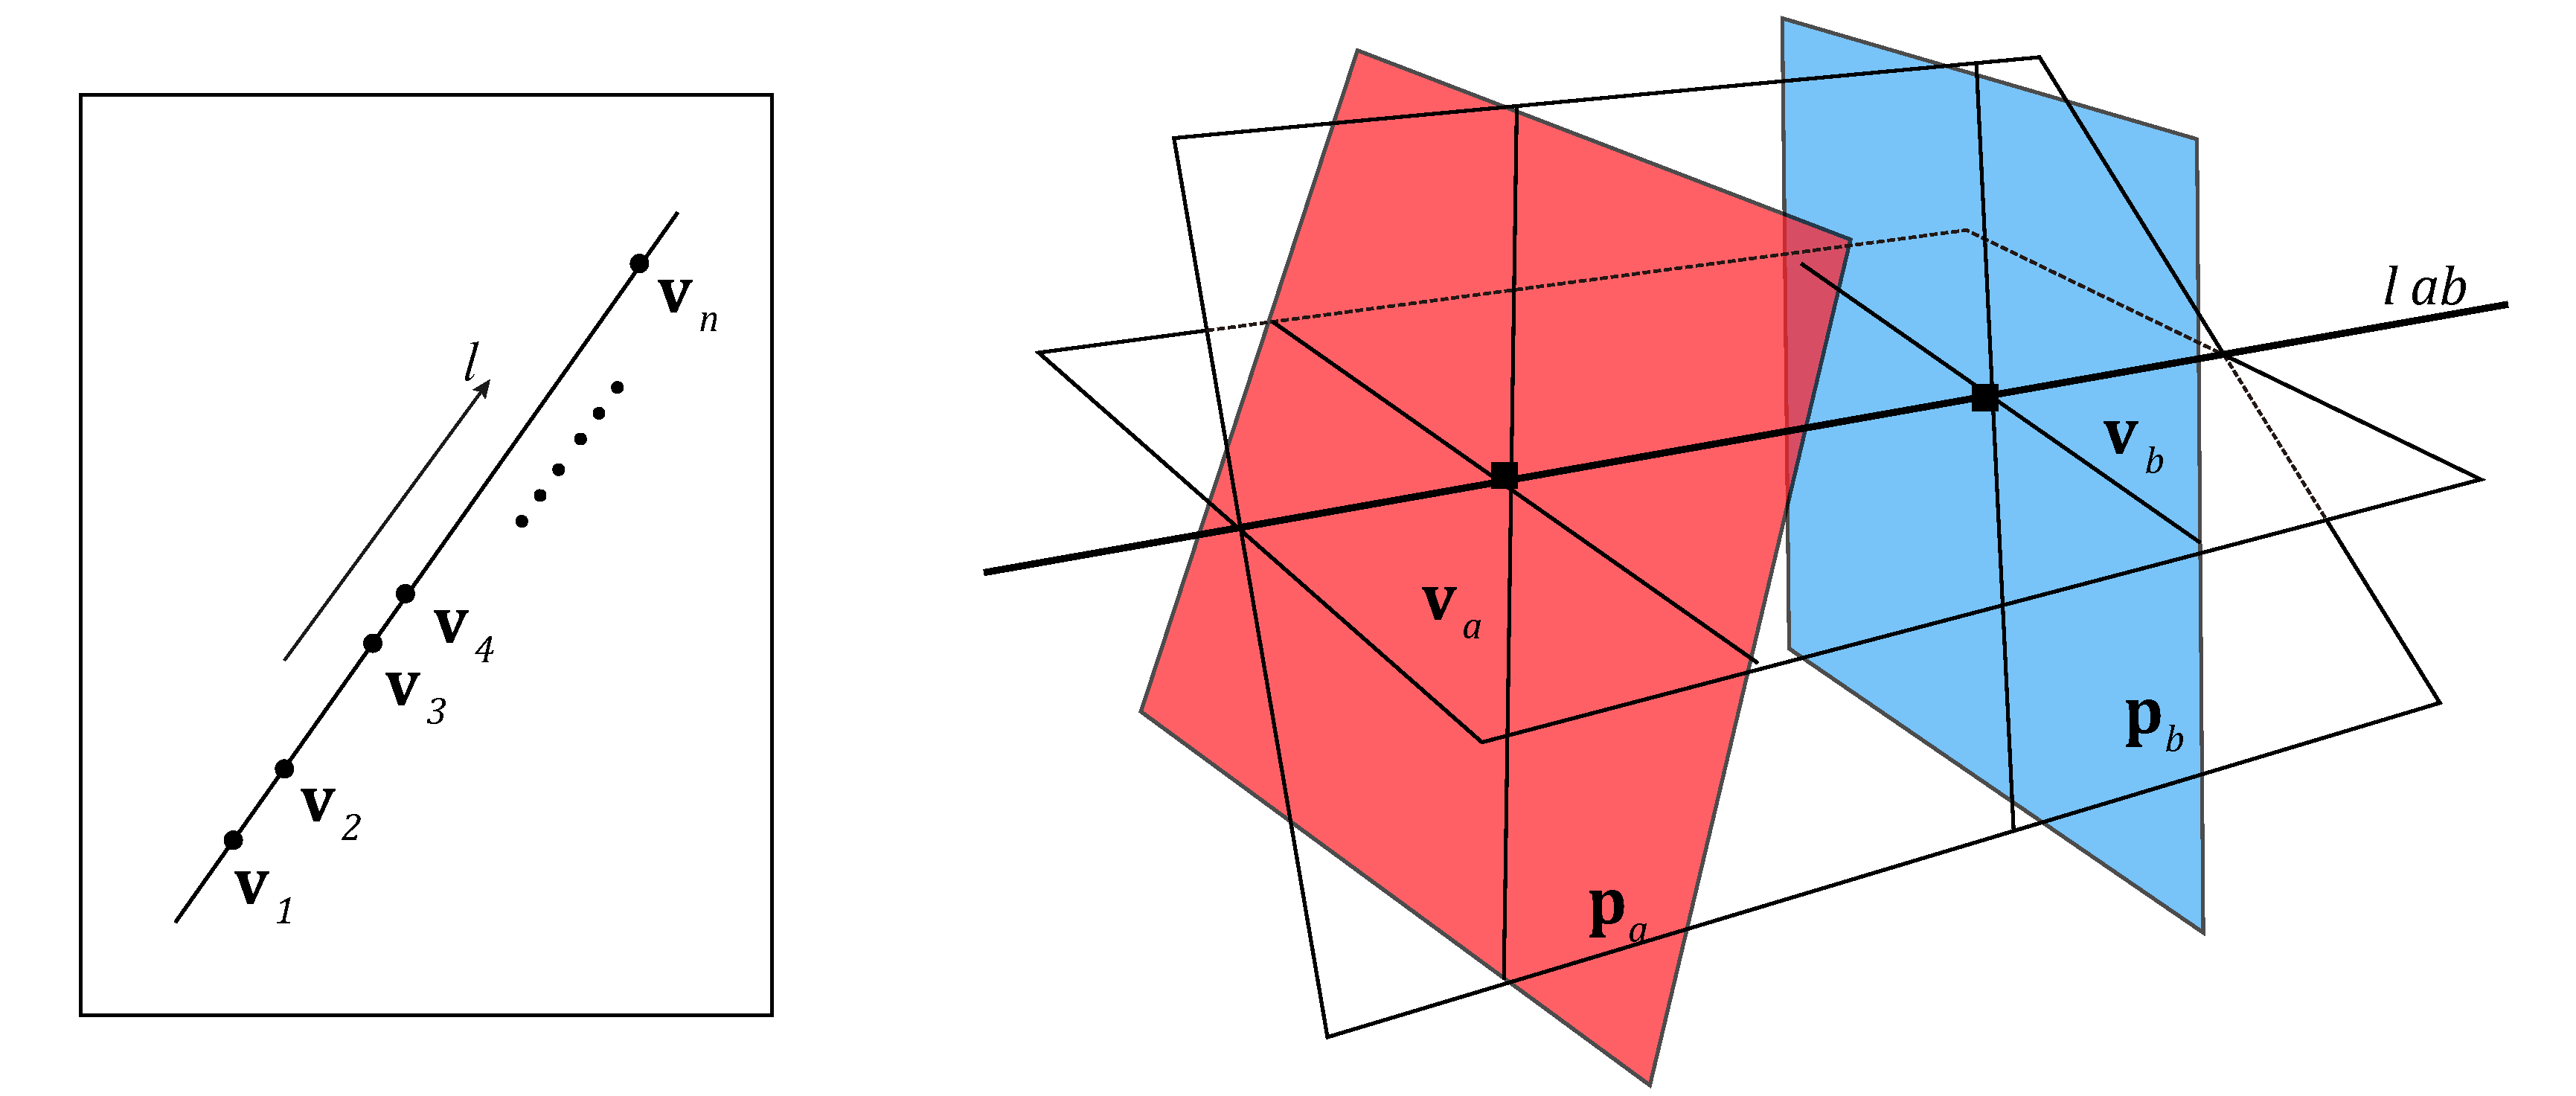
\includegraphics[width=3.5in]{twopointoneline}\\
  \caption{Geometry configuration of linear ordering of points. Points $\bm{v}_a$ and $\bm{v}_b$ are both on line $\bm{l}_{ab}$. We convert this problem into the plane ordering of $\bm{p}_a$ and $\bm{p}_b$ along $\bm{l}_{ab}$.}\label{fig:twopointoneline}
\end{figure}


\noindent Given an line $\bm{l}_{ab}$ with two points $\bm{v}_a\colon(\bm{p}_a^0\cap\bm{p}_a^1\cap\bm{p}_a^2)$ and $\bm{v}_b\colon(\bm{p}_b^0\cap\bm{p}_b^1\cap\bm{p}_b^2)$ on it, we need to determine the linear order of the two points along $\bm{l}_{ab}$ (Fig. \ref{fig:twopointoneline}). To solve this problem, we choose one plane not parallel with $\bm{l}_{ab}$ from the plane representation of each point and convert this problem into linear order of planes, which can be solved by Banerjee et al.'s method \cite{banerjee1996topologically}. The chosen planes should have the same orientation with $\bm{l}_{ab}$ (the dot product between plane normal and $\bm{l}_{ab}$ has to be positive) and unqualified planes have to be flipped.


\begin{wrapfigure}{r}[0in]{0in}
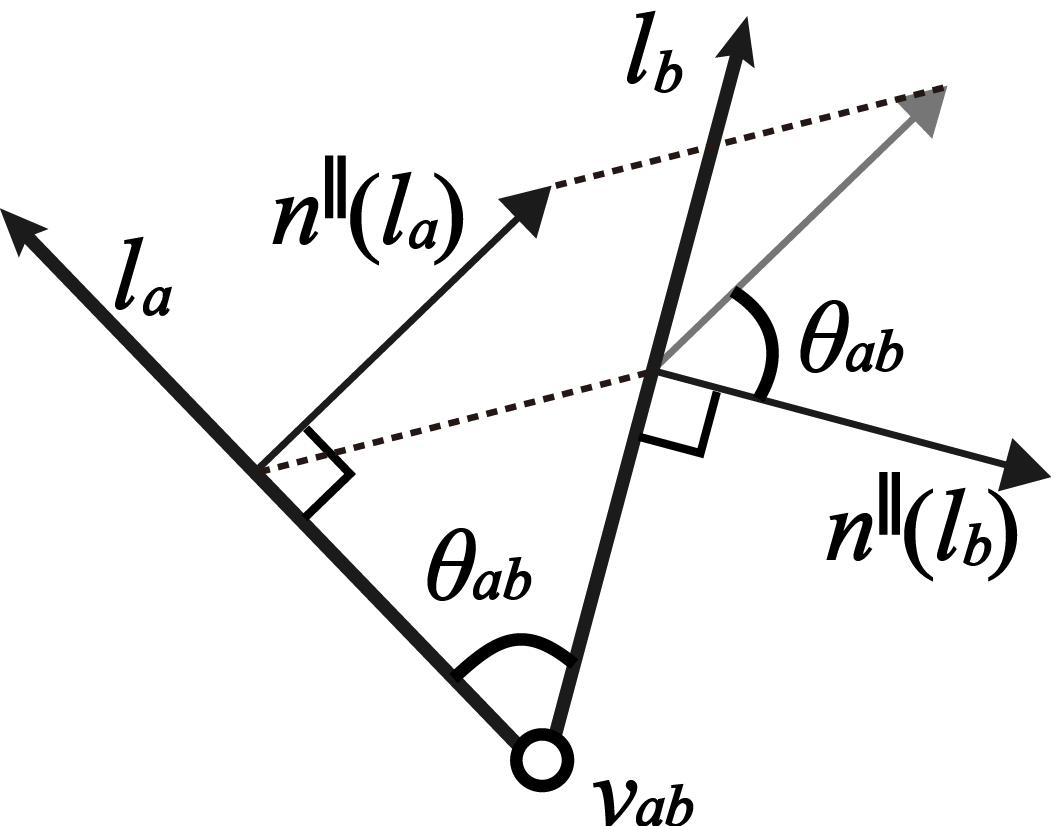
\includegraphics[width=1.5 in]{boolean-02}
%\caption{Plane-based representation of triangle}
\end{wrapfigure}
\vspace{0.5em}
\noindent \textbf{Circular ordering of lines}~~~~

\noindent During face tessellation, we need to know the which edges are neighboring (Fig. \ref{fig:circularorder}), that is, circular ordering of directed lines around a vertex. Lines can be sorted in a divide-and-conquer way based on the relative order of each pair of lines. Therefore, this problem is converted to that given two lines $\bm{l}_a$ and $\bm{l}_b$ in a plane $\bm{p}_0$ and their intersection point $\bm{v}_{ab}$, compute the circular order of the two lines. We can compute the order by the sign of $\sin{\theta_{ab}}$, where $\theta_{ab}\in(-\pi,\pi)$ is the angle from $\bm{l}_a$ to $\bm{l}_b$ under the top view of $\bm{p}_0$. The sign of $\sin{\theta_{ab}}$ is the same as triple product $\bm{n}(\bm{p}_0) \cdot (\bm{l}_a\times\bm{l}_b)$. However, explicit computing this equation is complicated because both $\bm{l}_a$ and $\bm{l}_b$ are implicitly represented by intersection of planes.

We develop an easier way that requiring no explicit computation of $\bm{l}_a$ and $\bm{l}_b$. First, we write the P-reps of two lines as $\bm{l}_a\colon(\bm{p}_0\cap\bm{p}_a)$ and $\bm{l}_b\colon(\bm{p}_0\cap\bm{p}_b)$. Then we orthogonally decompose $\bm{n}(\bm{p}_a)$ and $\bm{n}(\bm{p}_b)$ along $\bm{n}(\bm{p}_0)$:
\begin{equation}
\begin{split}
&\bm{n}(\bm{p}_a)= \bm{n}^\parallel(\bm{p}_a) + \bm{n}^\perp(\bm{p}_a)\\
&\bm{n}(\bm{p}_b)= \bm{n}^\parallel(\bm{p}_b) + \bm{n}^\perp(\bm{p}_b)
\end{split}
\end{equation}
Here superscript `$\parallel$` means the projection on $\bm{p}_0$ and `$\perp$` means orthogonal to $\bm{p}_0$. As we know $\bm{n}^\perp(\bm{p}_a)$ and $\bm{n}^\perp(\bm{p}_b)$ are both parallel to $\bm{n}(\bm{p}_0)$, we get:
\begin{equation}
\label{eq:circ1}
\bm{n}(\bm{p}_0) \cdot (\bm{n}(\bm{p}_a) \times \bm{n}(\bm{p}_b)) = \bm{n}(\bm{p}_0) \cdot (\bm{n}^\parallel(\bm{p}_a) \times \bm{n}^\parallel(\bm{p}_b)).
\end{equation}
By observation we find that the angle between $\bm{n}^\parallel(\bm{p}_a)$ and $\bm{n}^\parallel(\bm{p}_b)$ is exactly $\theta_{ab}$. So the sign of the right side of equation \ref{eq:circ1} is exactly the sign of $\sin{\theta_{ab}}$. It means we have the following nice conclusion:
\begin{equation}
\label{eq:circ2}
sign(\sin{\theta_{ab}})=  sign(\bm{n}(\bm{p}_0)\cdot(\bm{n}(\bm{p}_a) \times \bm{n}(\bm{p}_b)))
\end{equation}

Since all the three vectors on the right side are already explicitly represented, we only have to evaluate the sign of an 3$\times$3 matrix and avoid complicated arbitrary precision float-point arithmetic.

\begin{figure}[t]
\centering
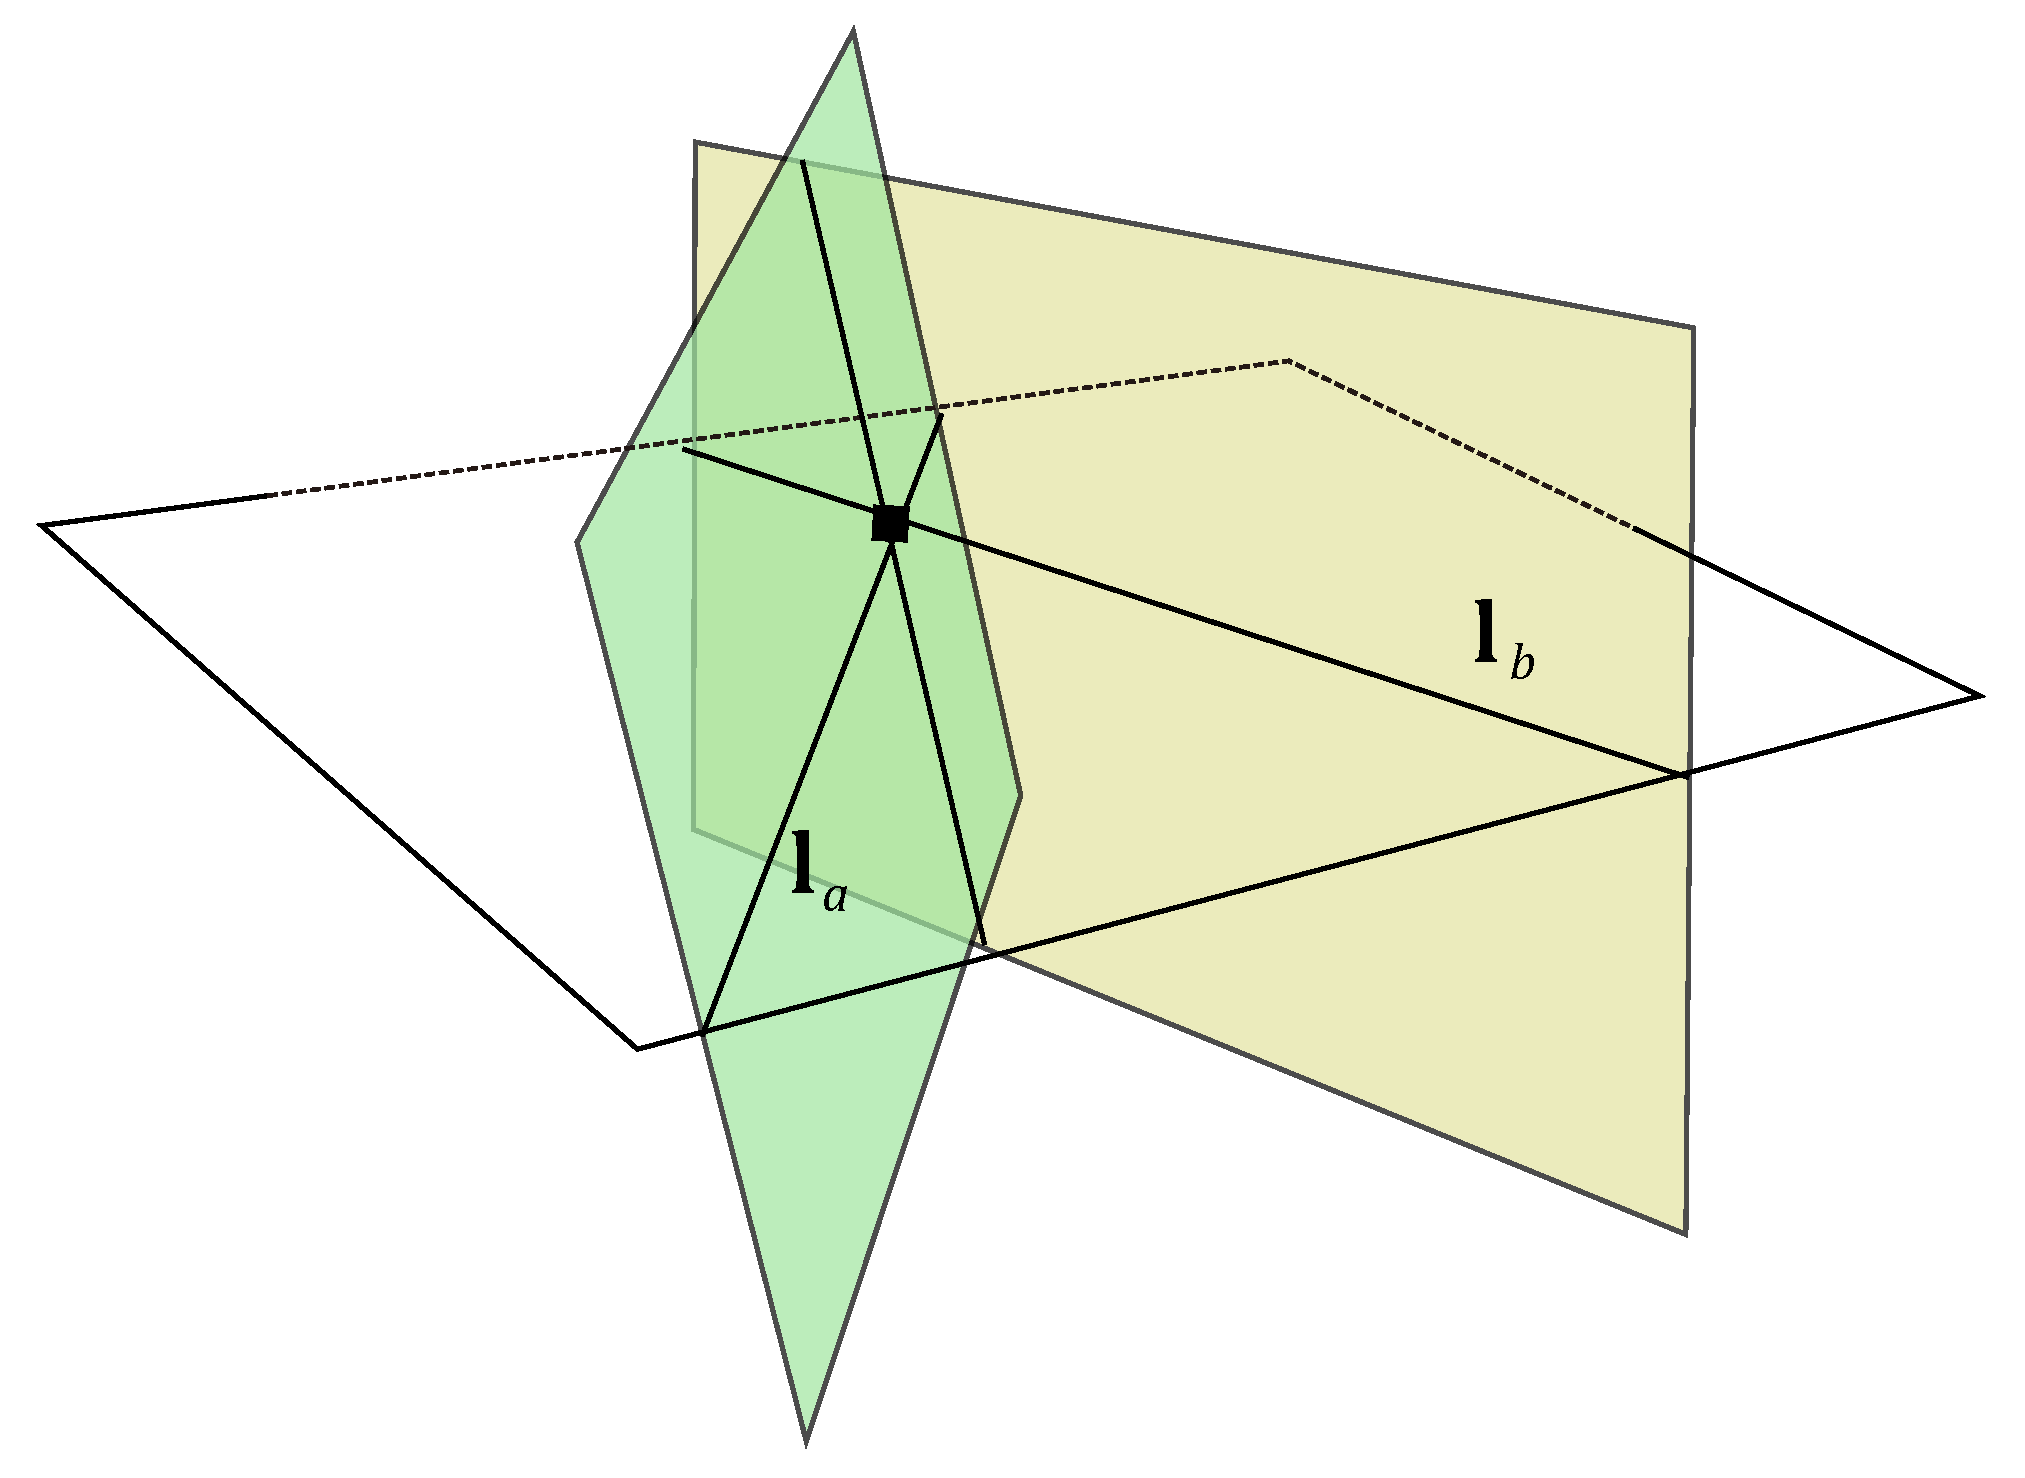
\includegraphics[width=3.5in]{circularorder}
\caption{Geometry configuration of circular ordering of lines. $\bm{l}_a\colon(\bm{p}_0 \cap \bm{p}_a)$ and $\bm{l}_b\colon(\bm{p}_0 \cap \bm{p}_b)$ are within plane $\bm{p}_0$.}
\label{fig:circularorder}
\end{figure}


\subsection{Method Overview}


There are generally three steps in our method. The first step is to compute intersections between each triangle face pairs. After that, the input meshes are tessellated into intersection-free meshes according to these intersections. The last step is to classify each face and generate the final result mesh.

\subsubsection{Intersection computation}

In this step, we only compute intersections between triangle pairs. The triangle-triangle intersection test is largely based on M\"{o}ller's algorithm \cite{moller1997fast} for its efficiency. However, conventional implementation of M\"{o}ller's algorithm using vertex-based geometry brings numerical errors. Therefore, we integrate P-rep into M\"{o}ller's algorithm. All intersection points and line segments are represented using planes to avoid explicitly computing the coordinates. Also, we carefully deal with degenerate cases of triangle intersections, including point intersections, edge intersections and coplanar situations. In addition, octree is used to speed up the whole process. Details are provided in \S\ref{section:isect}.

\subsubsection{Deferred tessellation}

Once all intersections between triangles are detected, we need to tessellate the input meshes and construct the intersection-free meshes. In many methods like \cite{ogayar2015deferred}, constraint Delaunay triangulation (CDT) is applied to perform tessellation. However, for a CSG with more than two meshes, intersections may overlap or intersect with each other, and cannot be used for constraints of CDT directly. In addition, as our intersections are represented by planes, implementation of CDT are complex and inefficient, as most CDT algorithms (e.g. \cite{chew1989constrained}, \cite{de1992line}) is not designed to handle planes and requires explicit coordinates. Therefore, we first perform intersection refinement to resolve intersecting intersections. After that, we construct a graph-like structure suitable for P-rep intersections, called \emph{tess-graph}, to guide the exact tessellation of each face. After all faces are tessellated, we get our intersection-free meshes. Details are shown in \S\ref{sec:tessellation}.

\iffalse
\begin{figure}
  \centering
  % Requires \usepackage{graphicx}
  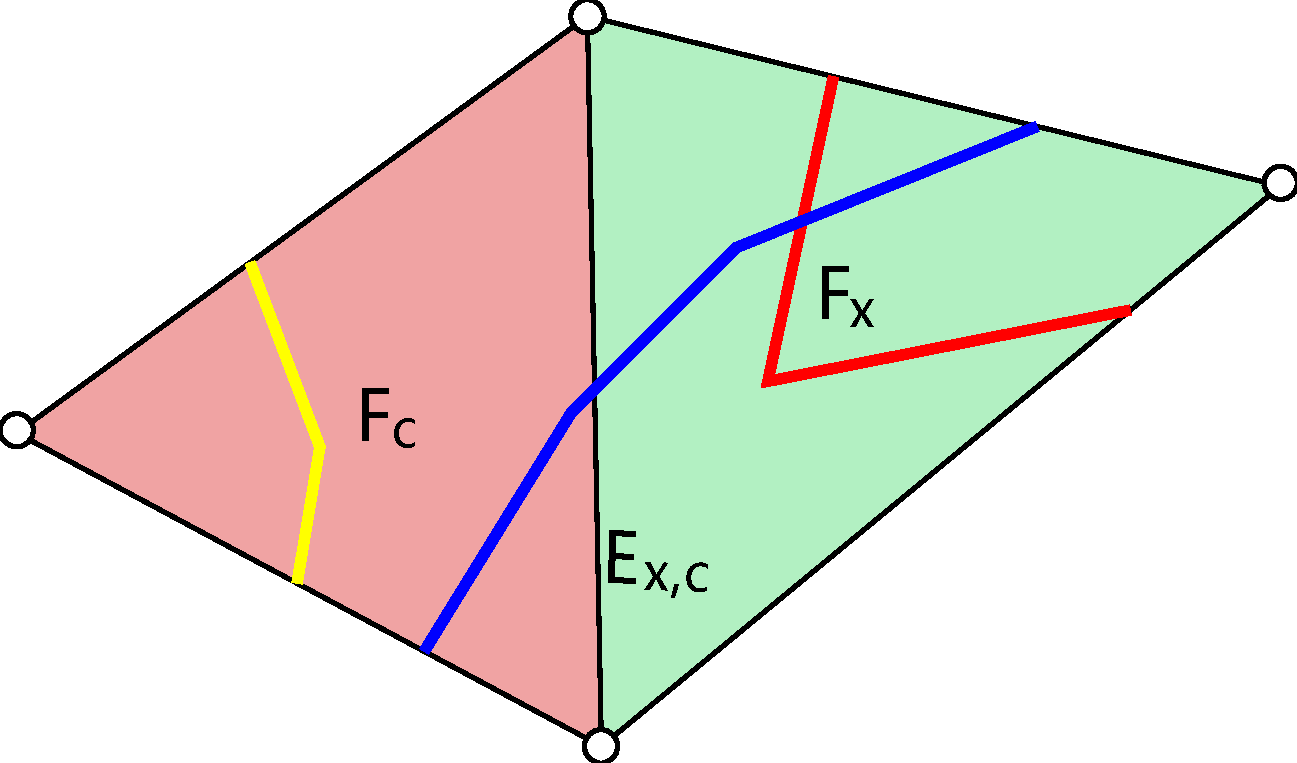
\includegraphics[width=1.7in]{sgen}\\
  \caption{Triangle-triangle intersections made by different triangle pairs may (a) overlap or (b) intersect with each other. (c) Such situation introduces extra vertex which is intersection of triangles from three different meshes.}\label{fig:p-reps}
\end{figure}
\fi

\subsubsection{Face classification}

This step is to choose faces from the intersection-free meshes to generate the final mesh. However, literally computing the indicator vector of each face is unacceptably slow for large CSGs. We utilize the geometry connectivity stored in B-reps to propagate indicators in a flood-filling manner. In addition, many methods use barycenters of faces together with point-in-polyhedra test for face classification, which is not exact nor robust with fix-precision float-point arithmetics. Different from them, we classify faces based on the classification results of exactly represented vertices, including input vertices and newly introduced intersection vertices, and carefully deal with coplanar conditions to ensure topology consistency. Details will be shown in \S\ref{sec:classification}.

\begin{figure}[t]
\centering
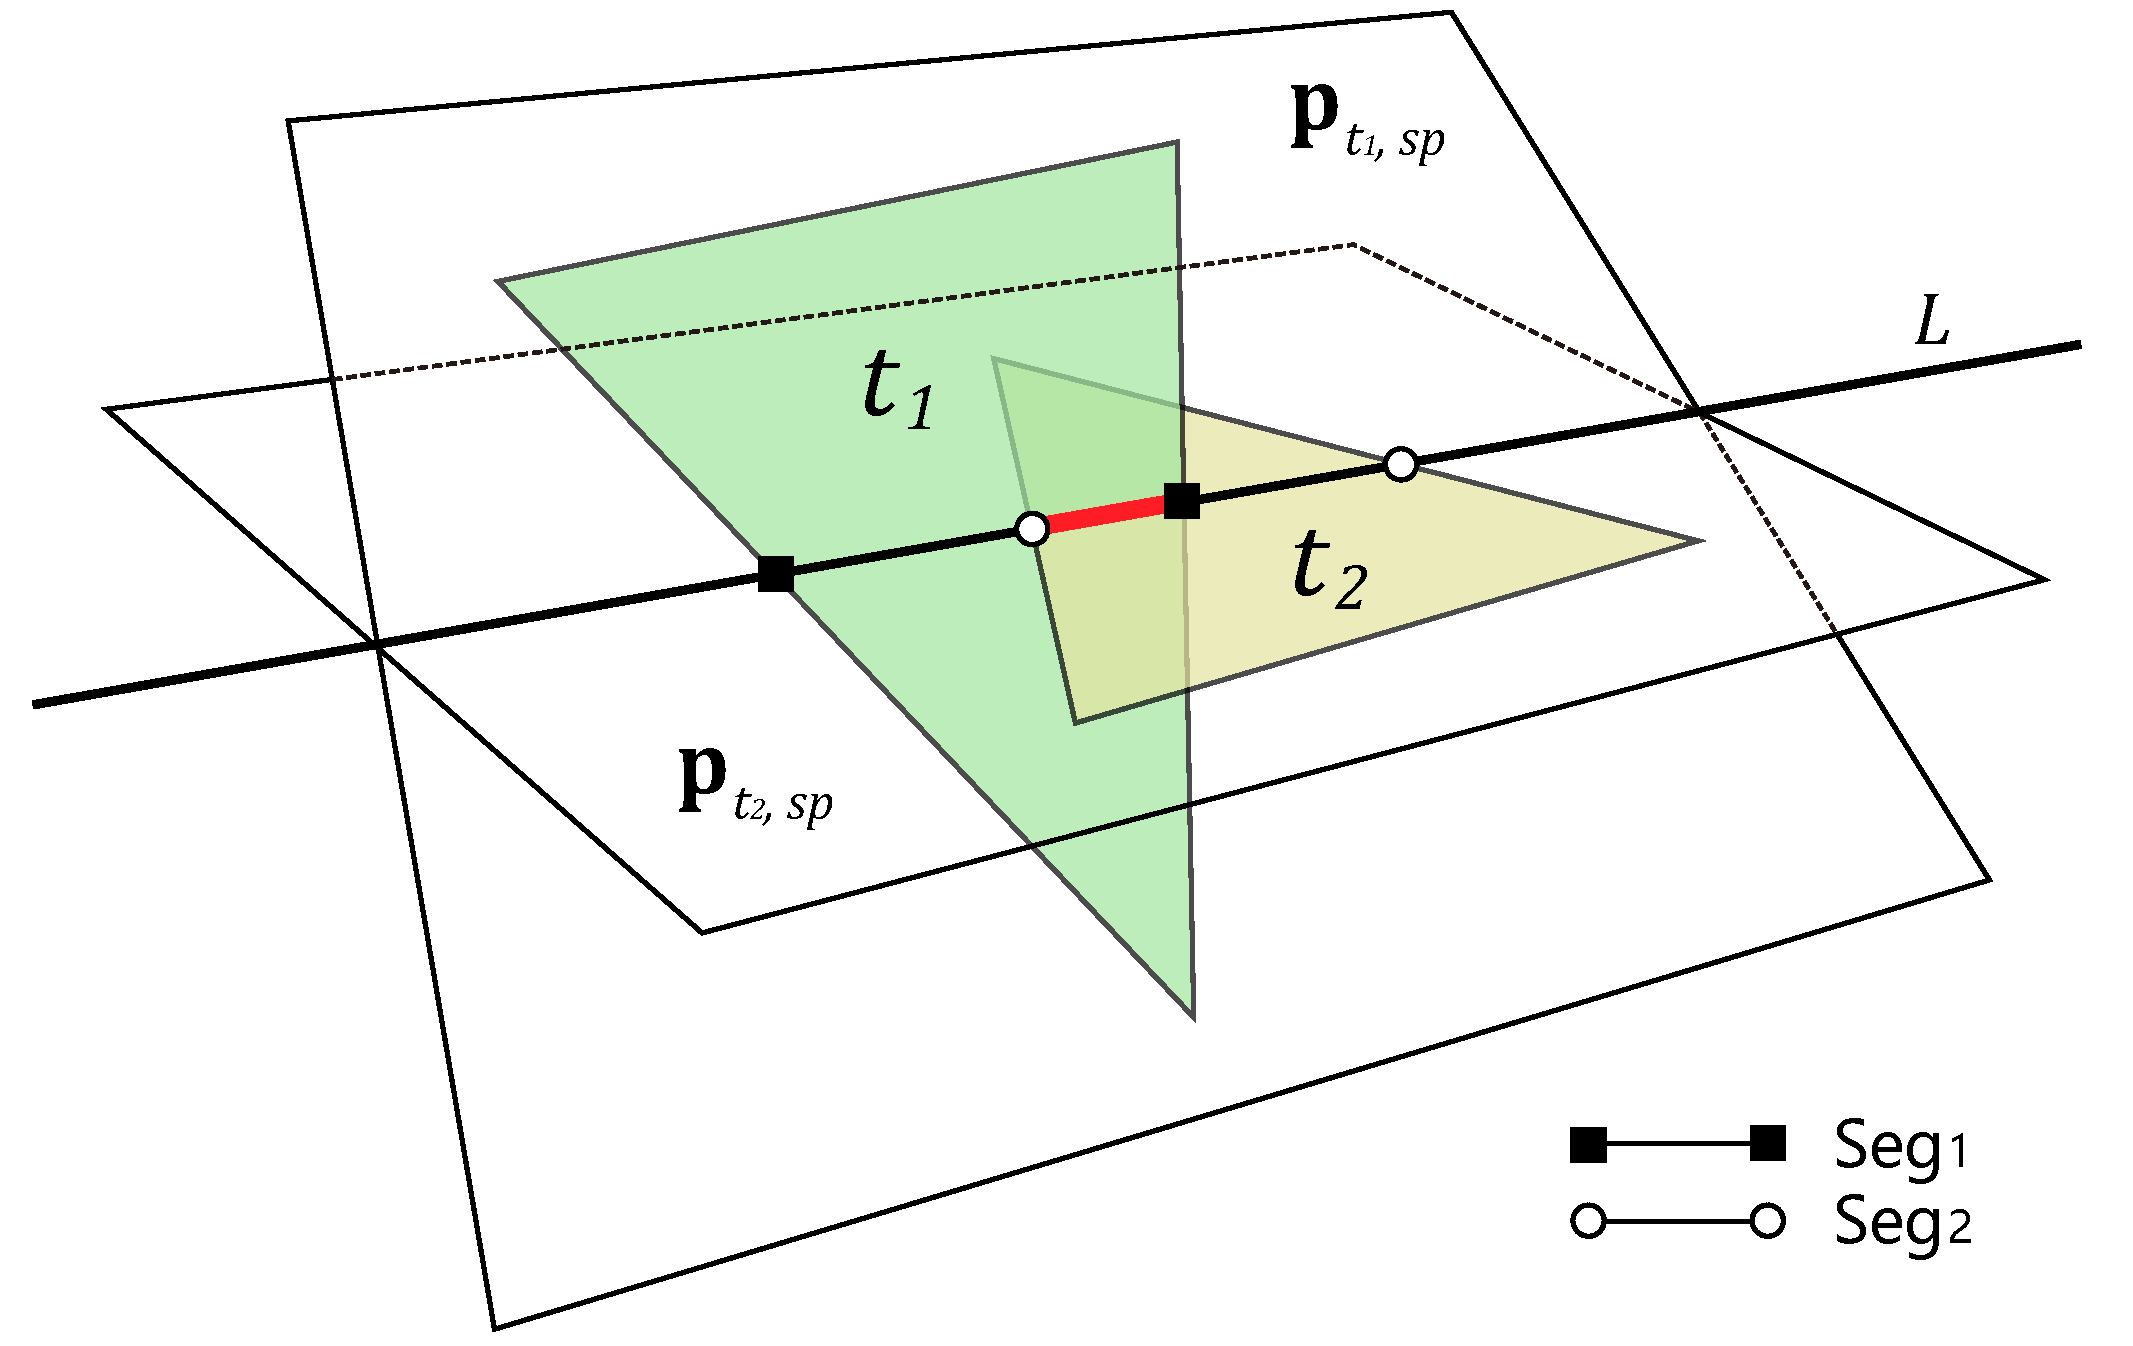
\includegraphics[width=2.5in]{projection}
\caption{$Seg_1$ is the intersection between $\bm{p}_{t_2, sp}$ and $t_1$. $Seg_2$ is the intersection between $\bm{p}_{t_1, sp}$ and $t_2$. The intersection between $t_1$ and $t_2$, which is the line segment in yellow, is the overlap of $Seg_1$ and $Seg_2$.}
\label{fig_projection}
\end{figure}
\section{Intersection Computation}

\label{section:isect}
In this step, intersections between faces are computed through triangle-triangle intersection test. We adopt M\"{o}ller's algorithm \cite{moller1997fast} on account of its efficiency and simplicity. However, a naive implementation of M\"{o}ller's algorithm can introduce numerical errors and may fail to produce correct results. Therefore, we integrate plane-based geometry to make it exact. In the following, we first introduce our space division strategy to reduce the number of intersection test. Then we make a quick review of M\"{o}ller's algorithm, and discuss the way to embed plane-based geometry. After that, we discuss how to deal with degenerate cases.



\subsection{Space Division}
\begin{wrapfigure}{r}[0in]{0in}
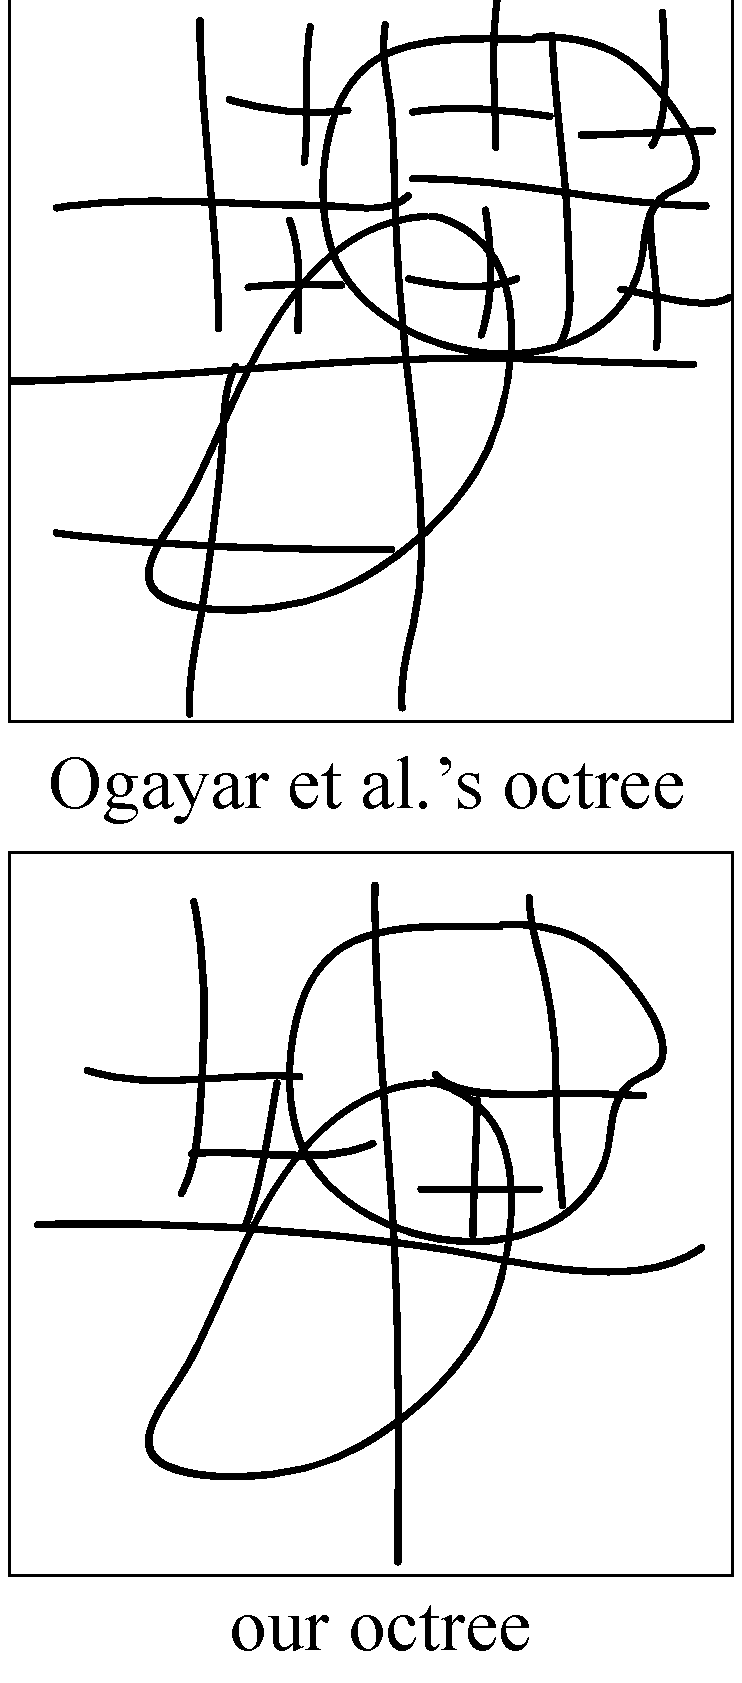
\includegraphics[width=1.2in]{octreediff}
\end{wrapfigure}
As intersection detection is performed between each pair of faces, localization is necessary for large CSGs to reduce the number of testing pairs. We use the adaptive octree for this purpose. Our implementation is akin to the implementation in Ogayar et al.'s method \cite{ogayar2015deferred}. Intersection between triangle faces and octree nodes are efficiently detected using the separating axis theorem \cite{gottschalk1996obbtree}. Octree leaves are classified into two types: if all faces that intersect a leaf belong to the same mesh, we call it a \emph{normal cell}. Otherwise, it is a \emph{critical cell}, within which the following intersection computation is performed.

The difference between our octree and Ogayar et al.'s is that we do not subdivide any normal cell no matter how many faces it contains. This is because subdividing normal cells benefits only the point-in-polyhedron test  \cite{frisken2002simple}, which seldom uses in our method. This simplification can save much computing time, especially when intersections between primitives are not complex and located in small regions.


\subsection{M\"{o}ller's Vertex-Based Method}



M\"{o}ller's algorithm computes the intersection between two triangles $t_1$ and $t_2$ in three steps as shown in Fig. \ref{fig_projection}:
\begin{itemize}[leftmargin=0.45cm]
\item[1)] An early rejection is performed by testing whether $t_1$ intersects $\bm{p}_{t_2, sp}$, the supporting plane of $t_2$. The same test is also done between $t_2$ and $\bm{p}_{t_1, sp}$.
\item[2)]The intersection between $t_1$ and $\bm{p}_{t_2, sp}$, denoted as $Seg_1$, and the intersection between $t_2$ and $\bm{p}_{t_1, sp}$, denoted as $Seg_2$, are separately computed .
 \item[3)]The intersection between $t_1$ and $t_2$ is determined by computing the overlap between $Seg_1$ and $Seg_2$ .
\end{itemize}

The non-robustness of this algorithm is from computing the coordinates of intersection vertices, which is the end points of $Seg1$ and $Seg2$. Although implementation with arbitrary precision arithmetic produces exact coordinates, it is too costly for boolean operations of large CSG. We use plane-based geometry to solve this problem by implicitly representing intersections with planes.


\subsection{Plane-Based Intersection}

\label{sec:embed}
Given a triangle face $t$, it is firstly converted to its P-rep: a supporting plane $\bm{p}_{t, sp}$ surrounded by three bounding planes $\{\bm{p}_{t, b}^i|\ i = 0,1,2\}$. We integrate the plane-based geometry into each of the tree steps of M\"{o}ller's algorithm as following:

\begin{figure}[t]
\centering
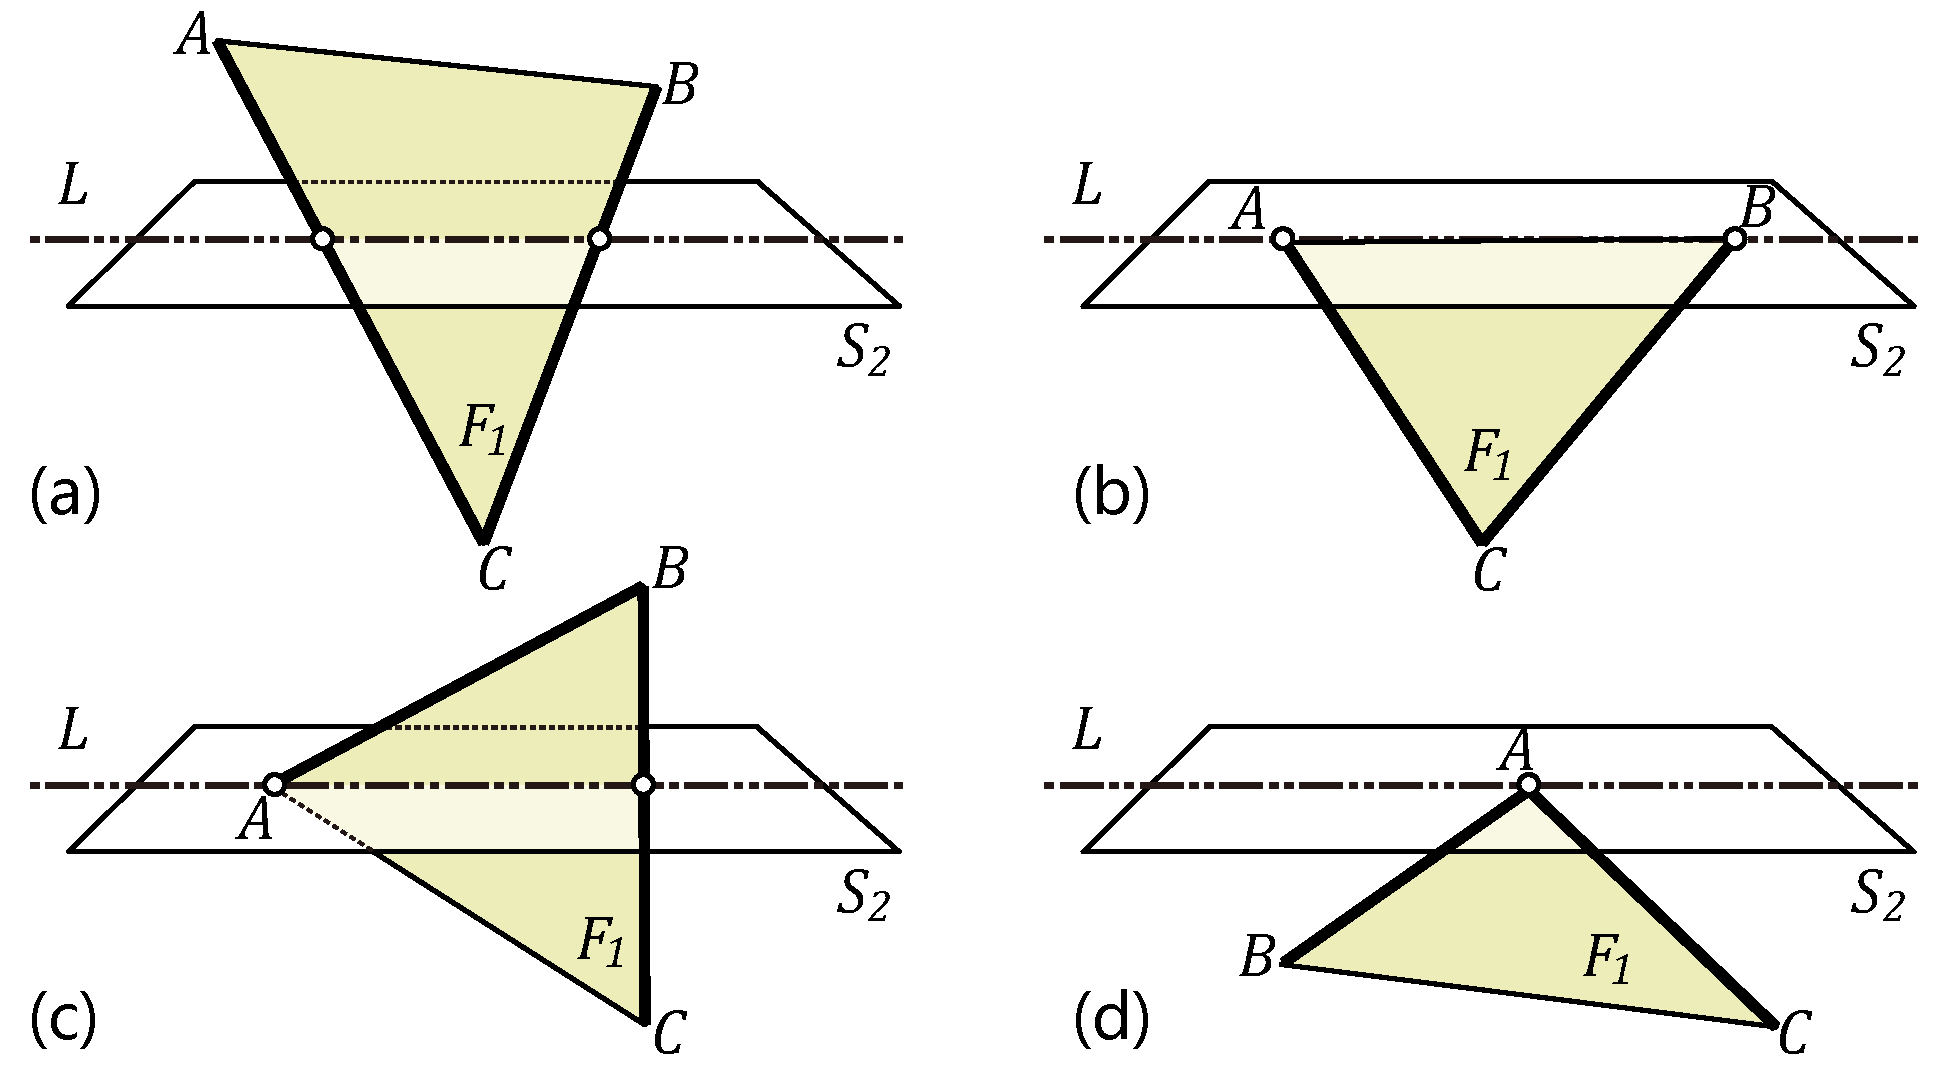
\includegraphics[width=3.5in]{sign}
\caption{We denote the signed distance from point $v_i$ to plane $\bm{p}_{t_2, sp}$ as $d_i$. All the four conditions of intersection between $t_1$ and $\bm{p}_{t_2, sp}$ are:  (a) $d_0\cdot d_2<0$, $d_1\cdot d_2<0$; (b) $d_0=0$, $d_1=0$, $d_2\neq 0$; (c) $d_0=0$, $d_1\cdot d_2<0$; (d) $d_0=0$, $d_1\cdot d_2>0$. End points of $Seg_1$ are intersections between $\bm{p}_{t_2, sp}$ and related edges of $t_1$ (red bold lines).}
\label{fig:isect}
\end{figure}



\begin{itemize}[leftmargin=0.45cm]
  \item[1)] The basic subroutine of the first step is to compute the orientation of of a face with respect to vertices of the other face. We find that since the exact coordinates of each triangle vertices are known, we can compute the point-plane orientation using vertex-based geometry predicates. This allow us to perform this early rejection efficiently.
      \vspace{0.5em}
  \item[2)] If $t_1$ and $t_2$ are not coplanar, the end points of $Seg_1$ and $Seg_2$ can be implicitly represented by plane triples. Take $Seg_1$ as an example. $Seg_1$ is the intersection between $t_1$ and $\bm{p}_{t_2, sp}$ and the end points of $Seg_1$ are intersections between $\bm{p}_{t_2, sp}$ and edges from $t_1$ (denoted as $\bm{e}^i_{t_1}, i\in\{0,1,2\}$). Because $\bm{e}^i_{t_1}$ can be represented as $\bm{p}_{t_1, s}\cap \bm{p}^i_{t_1, b}$, the end points of $Seg_1$ can be represented in the form of $\bm{p}_{t_2, sp} \cap \bm{p}_{t_1, sp} \cap \bm{p}^i_{t_1, b}$. In Fig. \ref{fig:isect}, we list all possible intersecting situations between $t_1$ and $\bm{p}_{t_2, sp}$ and the corresponding $\bm{e}^i_{t_1}$. The coplanar situation will be discussed later in \S \ref{sec:degenerate}.
      \vspace{0.5em}
 \item[3)] The intersection between $t_1$ and $t_2$ is the overlap area of $Seg_1$ and $Seg_2$. It can be easily computed by sorting the end points of $Seg_1$ and $Seg_2$ along the line $\bm{l}\colon \bm{p}_{t_1, sp} \cap \bm{p}_{t_2, sp}$. Because end points are all represented using plane triples, we can use the linear order of points discussed in \S \ref{sec:substrates} to sort.
\end{itemize}

Each time an intersection is computed, two intersections are generated (one for each triangle) and the newly generated vertices are added into meshes. To avoid repetitive vertices in the final result, we perform vertex repetition elimination in this step, merging coincident vertices even if they come from different input meshes. Because we use P-reps, the comparison of vertices is exact.

\subsection{Plane-Based Intersection Representation}
\label{sec:ir}

In our method, intersection on triangle $t$ is stored as $\bm{\mathcal{I}}\colon\{T, \bm{P}_{ext}, (\bm{P}_0, \bm{P}_1), \mathcal{N}\}$, which is called plane-based intersection representation (PBI-rep,  see Fig. \ref{fig:pbi}). The first component $T$ indicates which triangle $\bm{\mathcal{I}}$ lies on. $\bm{P}_{ext}$ indicates $\bm{\mathcal{I}}$ lies on $\bm{P}_{ext}$, which also means it lies on line $\bm{p}_{t, sp} \cap \bm{P}_{ext}$. The two end points of $\bm{\mathcal{I}}$ are $\bm{p}_{t, sp} \cap \bm{P}_{ext}\cap\bm{P}_0$ and $\bm{p}_{t, sp} \cap \bm{P}_{ext}\cap\bm{P}_1$. The last component $\mathcal{N}$ represents the neighborhood of the intersection $\bm{\mathcal{I}}$. It indicates $\bm{\mathcal{I}}$ is intersection of triangle $t$ with $\mathcal{N}$ from other mesh, where $\mathcal{N}$ can be either a face or a set of faces sharing the same edges.

\begin{figure}[t]
\centering
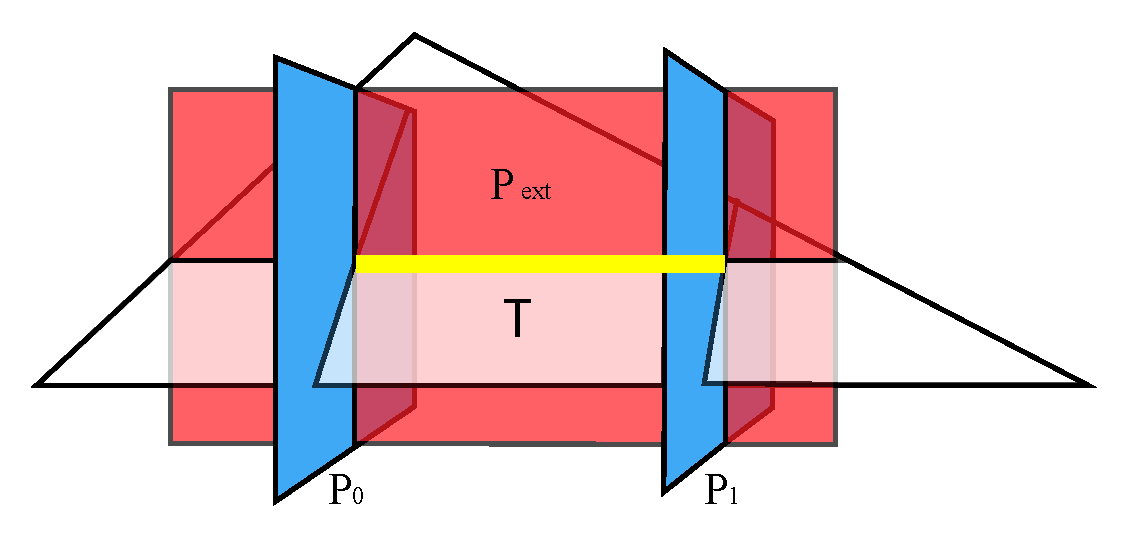
\includegraphics[width=3in]{pbirep2}
\caption{The geometry meaning of planes in a PBI-rep. The yellow line segment is the represented intersection.}
\label{fig:pbi}
\end{figure}

For example, two triangle faces $t_1$ and $t_2$ from mesh $M_i$ and $M_j$ intersect. Then it generates two intersections--- ${\bm{\mathcal{I}}}_{12}$ on $t_1$ and ${\bm{\mathcal{I}}}_{21}$ on $t_2$. For ${\bm{\mathcal{I}}}_{12}$ on $t_1$, $T = t_1$ and $\bm{P}_{ext}=\bm{p}_{t_2, sp}$. The third component is boundary planes from $t_2$ which has already been discussed in \S\ref{sec:embed}. The last component is $\mathcal{N}=t_2$. Sometimes intersections may lie on the mesh edges instead of faces (Fig. \ref{fig:twin}), which is called 'edge intersection'. In that case, the second component of neighborhood is a set of adjacent faces. We postpone the discussion of edge intersection to \S\ref{sec:degenerate}.


\subsection{Degenerate Case Handling}
\label{sec:degenerate}

While two triangles, if intersecting, intersect on a line segment in most situations, they can also intersect on a point or a convex area (coplanar case). Even if the intersection is a line segment, the intersection can be on triangle edges. These degenerate situations prevent us from performing robust boolean operations. In this section, we offer simple but effective way to deal with all these degenerations, which conceals the complexity of intersections and simplifies later processing.

%The criterion of whether an intersection help tessellation is by its necessity: if the intersection is not presented, whether some faces from the linked halfedge will cross the boundary of primitives. The word 'cross' do not only include the situation that a face is partly outside and partly inside of a primitive, but also can mean that a face is partly inside (outside) and part on the boundary of the primitive.

\iffalse
\begin{figure}[t]
\centering
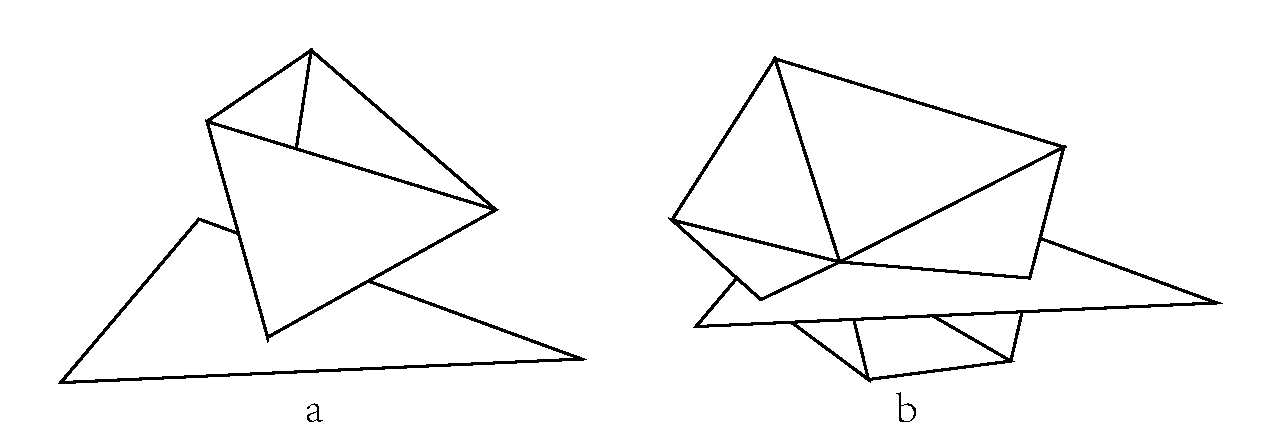
\includegraphics[width=3.5in]{isolated}
%\caption{Two situations of point intersections. (a) $\bm{v}_{iso}$ is isolated, and there is no adjacent intersection line segment. We need to add the $\bm{v}_{iso}$ to triangle $t_1$. (b) $\bm{v}_{non-iso}$ is not isolated. We do not need to add $\bm{v}_{non-iso}$ into $t_1$ because it can be added by other triangle pairs which intersect on line segments. However, for simplicity, we add the intersection point into $t_1$ in both situations.}
\label{fig:isolated}
\end{figure}
\fi

\subsubsection{Point intersection}
\label{sec:ipoint}
If two triangles intersect on a single point (e.g., Fig. \ref{fig:isect}d), the intersection cannot be represented using our four-component description since the line segment collapses into a single point. In these cases, we simply add the intersection point into the related triangles to guarantee correct tessellation. No intersection is introduced.



\subsubsection{Edge intersection}


When intersection line segment lies on the edge of face, we call it \emph{edge intersection}. The space near edge intersection is divided by faces around the intersected edge (typically two faces for a manifold edge), instead of just one face. Therefore, the neighborhood of the related intersection is a set of faces instead of a single one. For example, in Fig. \ref{fig:twin}, the neighborhood of the intersection on $t_1$ is $\{t_2, t^*_2\}$.

Another thing needs to be noticed is that there will be repetitive detection of edge intersections. For example, in Fig. \ref{fig:twin}a, the same intersection on $t_1$ will be detected twice because $t_1$ intersect both $t_2$ and $t_2^{\star}$ in exactly the same intersection. We solve this duplication together with other interactions among different intersections in \S\ref{sec:tessellation}. We also call such $t_2$ and $t_2^{\star}$ as \emph{companion triangles} in an edge intersection because they share the same edge intersection. This concept will be referred again in the discussion of coplanar cases.

\begin{figure}[t]
\centering
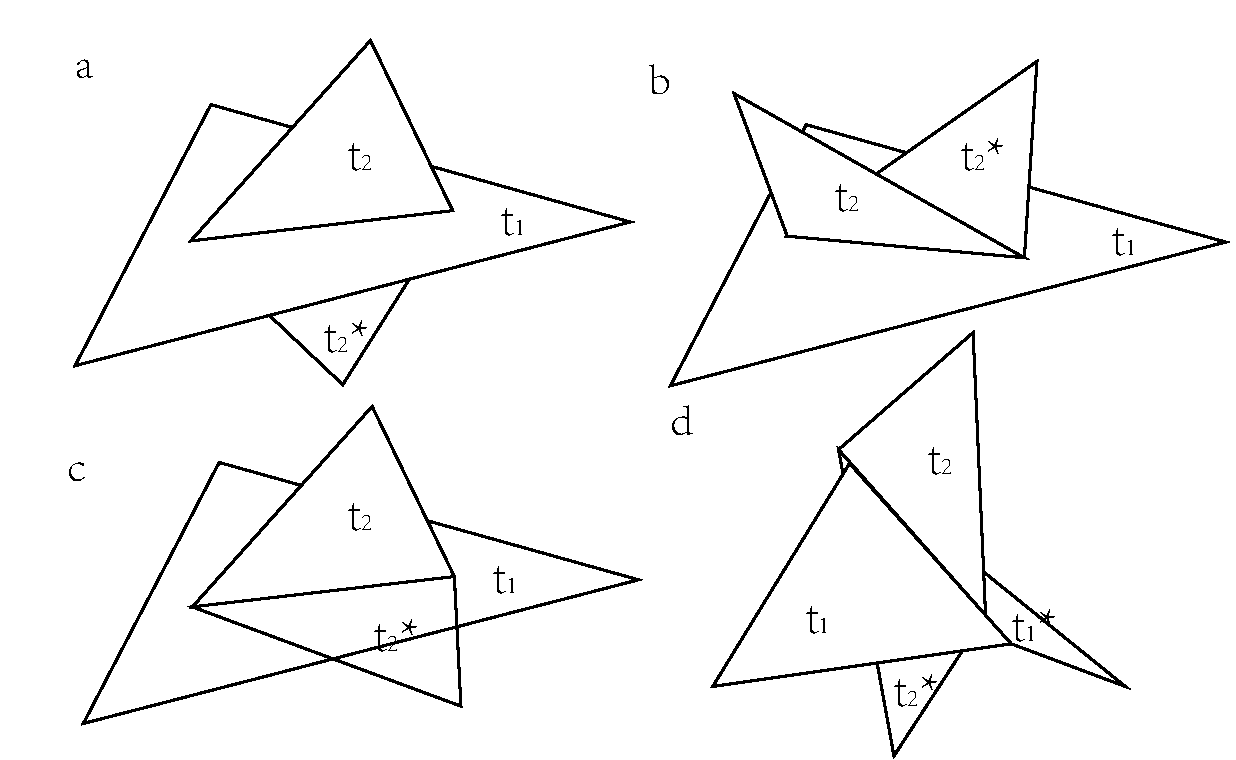
\includegraphics[width=3.5in]{edgeisect}
\caption{Different conditions of edge intersection. Triangle faces $t_1$ and $t_1^*$ are companion faces. Triangle faces $t_2$ and $t_2^*$ are companion faces. a) $t_2$ and $t_2^*$ are in different sides of $t_1$. b) $t_2$ and $t_2^*$ are in the same side of $t_1$. c) $t_2^*$ is coplanar with $t_1$. d) Both $t_1$ and $t_2$ have companion faces: the intersection is edge intersection for both $t_1$ and $t_2$ (instead of only for $t_2$ is previous three conditions). }
%\caption{Six situations of edge interse ctions. The first three subgraphs are edge-face intersections. The last three ones are edge-edge intersections. (a) Triangles are located in two sides, cross condition. (b) Triangles are located in the same sides, invalid condition. (c) One of the triangles are coplanar, coplanar condition. (d) Double twin intersections, cross condition. (e) Double twin intersections, coplanar condition. (f) Double twin intersections, coplanar condition.}
\label{fig:twin}
\end{figure}


\subsubsection{Copalnar}

\begin{figure}[t]
\centering
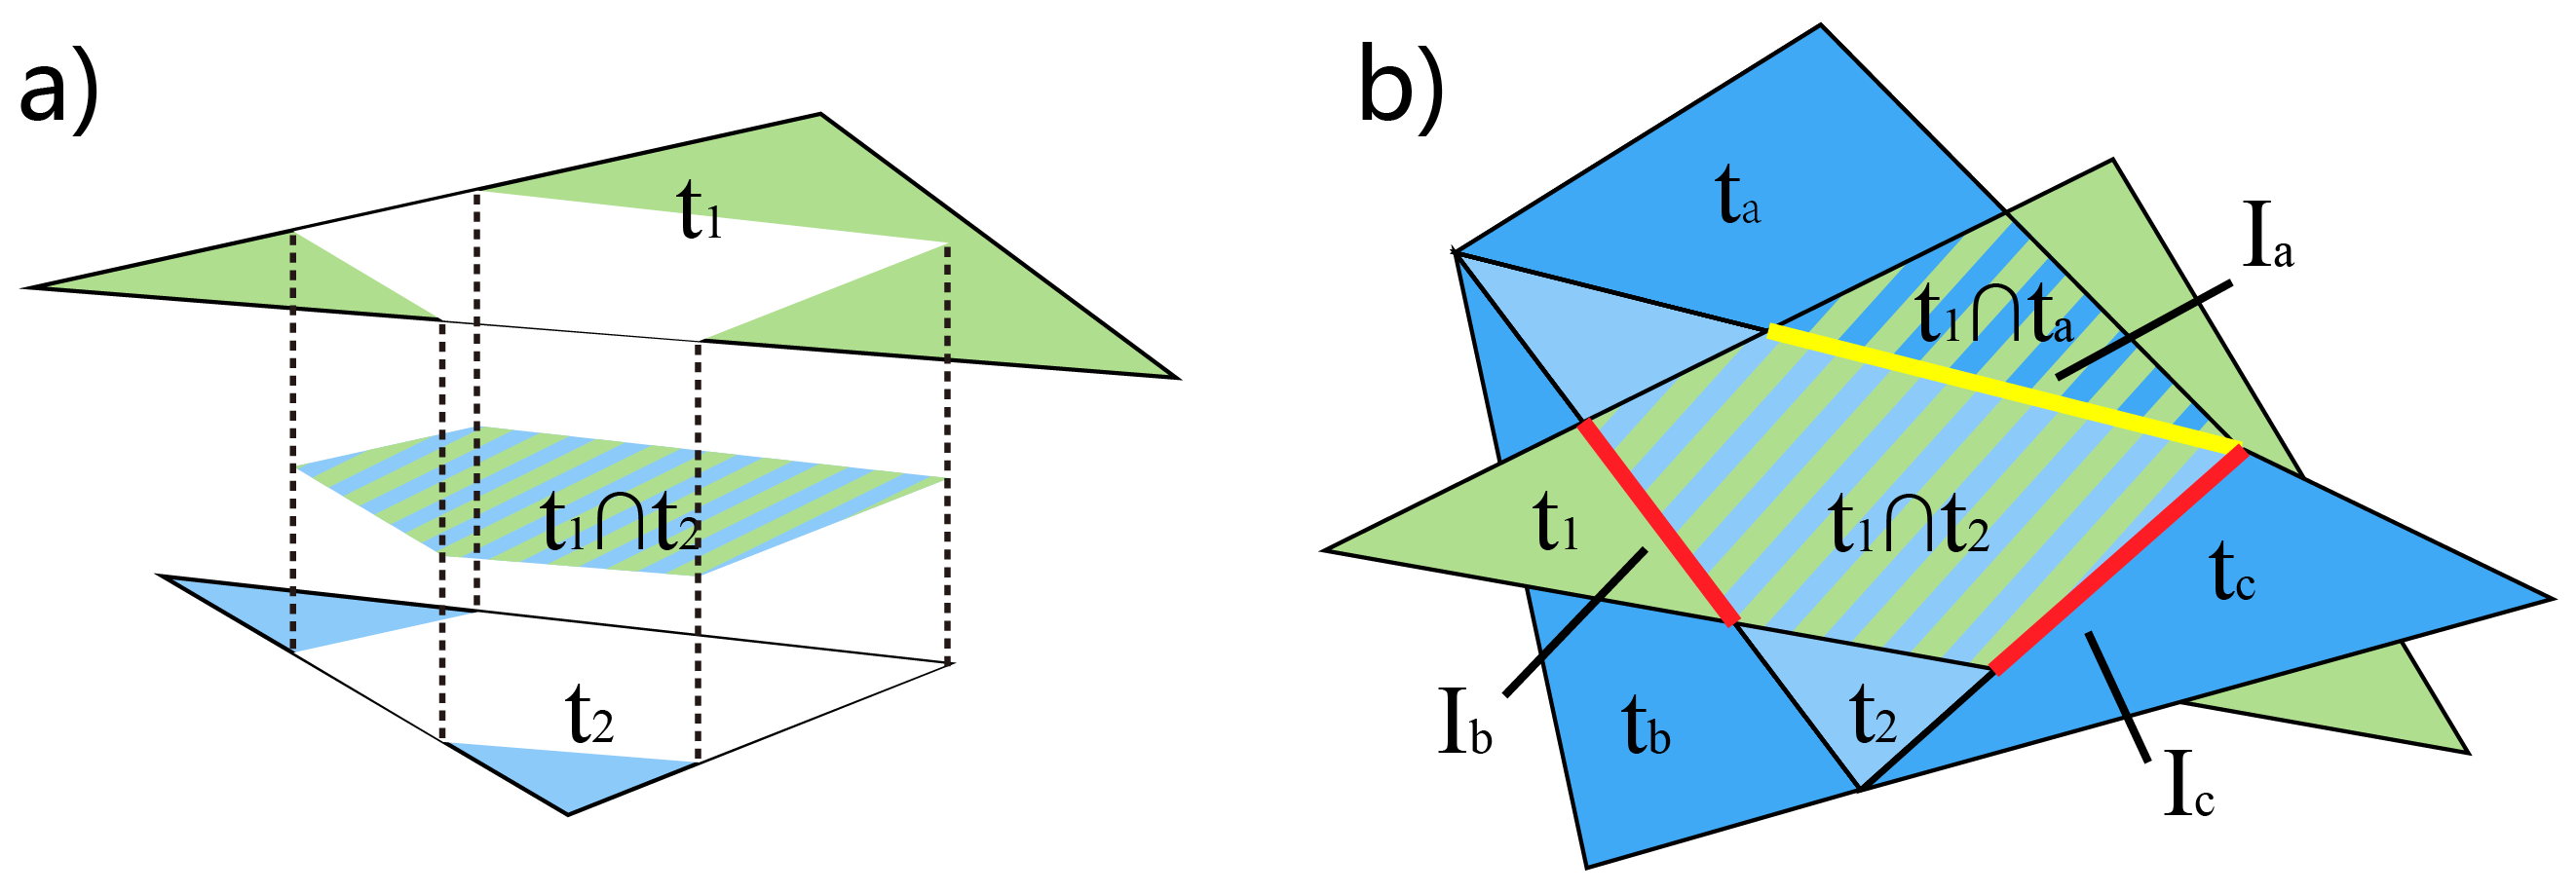
\includegraphics[width=3.5in]{boolean-03}
\caption{a) Coplanar cases, $t_a$ and $t_b$ intersect in 2D, dividing each other into two areas---a convex overlapping area and exclusive parts. b) The possible configurations of the companion faces. The blue triangles are from the same mesh. For $\mathcal{I}_1$, the companion triangle $t_1$ is coplanar with the $t-a$. Therefore, the overlap areas do not need to be split by the yellow edge during tessellation, thus $\mathcal{I}_1$ is invalid. For $\mathcal{I}_2$ and $\mathcal{I}_3$, the companion faces are not coplanar, so these intersection can be recorded during intersection test between $t_a$ and $t_1$ and $t_2$. In any configurations, their is no need to record the intersection between $t_a$ and $t_b$.}
\label{fig:coplanar}
\end{figure}

Consider two triangle faces $t_1$ and $t_2$ intersect within a common plane. Both $t_1$ and $t_2$ will divide each other into two areas---a convex overlapping area and exclusive parts (Fig. \ref{fig:coplanar}a). Apparantly, if we tessellate both $t_1$ and $t_2$ according to the boundary of overlapping area, we can guarantee that the tessellated meshes are intersection-free. Many previous methods \cite{feito2013fast,zhou2016mesh} use this method to guarantee topology correctness. However, in our method, we do not test whether $t_1$ and $t_2$ really intersect in 2D once we find they are coplanar. We treat coplanar situations as they do not intersect at all. In this way, we simplify our method, making it more robust and fast, while doing no harm to the topology correctness.

We find that each intersection line segment in 2D is part of the edges from input meshes. That means we can view 2D intersection as a special case of edge intersection. The only difference is that there can be up to three edge intersections in one 2D intersection (red and yellow line segments in Fig. \ref{fig:coplanar}b). As we have discussed, edge intersection will be detected twice. That means we can rely on the companion triangle faces to detect intersections.

However, if the companion triangles are also coplanar, neither of the two triangles will record the intersection. Fortunately, in this case, the intersection is not valid. The word `valid` means the intersections will appear as an edge in the final mesh, thus is necessary to put into tessellation. Supposing the intersection $\mathcal{I}$  is on triangle $t_1$, this definition equals to:
\begin{equation}
% = f(\bm{\Lambda}(\bm{s}_i))
\lambda_f(\bm{x}_i) \neq constant, \bm{x}_i \in \bm{U}(\mathcal{I}) \cup t_1
\end{equation}
, where $f$ is the CSG function, and $\bm{U}(\mathcal{I})$ is the the neighborhood of $\mathcal{I}$. This inequation indicates the two sides of $\mathcal{I}$ have different classification and must be split according to $\mathcal{I}$ during tessellation. However, in most time, the validation of intersection is not known until classification stage, because we have to know the indicator of each point in $\bm{U}(\mathcal{I}) \cup t_1$. Fortunately, if companion faces are both coplanar with $t_1$, both sides of $\mathcal{I}$ have the same indicator $on$ and thus the same classification. It means $\mathcal{I}$ is invalid and we do not need to record it.

\section{Deferred Tessellation}



\label{sec:tessellation}
After intersection computation, tessellation is performed on each intersecting triangle face and generate our intersection-free meshes. We call this stage as deferred tessellation because the tessellation happens until all valid intersections are computed.

Ogayar-Anguita et. al. \cite{ogayar2015deferred} use Constrained Delaunay Triangulation (CDT) to perform deferred tessellation. They treat triangle faces as convex triangulation zones and intersections as constraints. Our first try is to implement a robust plane-based CDT. However, CDT algorithms \cite{chew1989constrained,preparata2012computational} require coordinates projection or intersection detection between arbitrary connections of vertices within triangulation zone, which are difficult to be implemented under P-reps. From another perspective, CDT contains geometry constructions---new edges are generated to guarantee each subface is a triangle, which does not fit P-reps. Moreover, when there are more than two primitives, simply applying CDT omits the complexity of intersections between meshes. The intersections may intersect each other, introducing new vertices and splitting original intersection line segments (Fig. \ref{fig:iisect}a). This breaks the assumption of most CDT algorithms and may lead to incorrect output topology.

\begin{figure}[t]
\centering
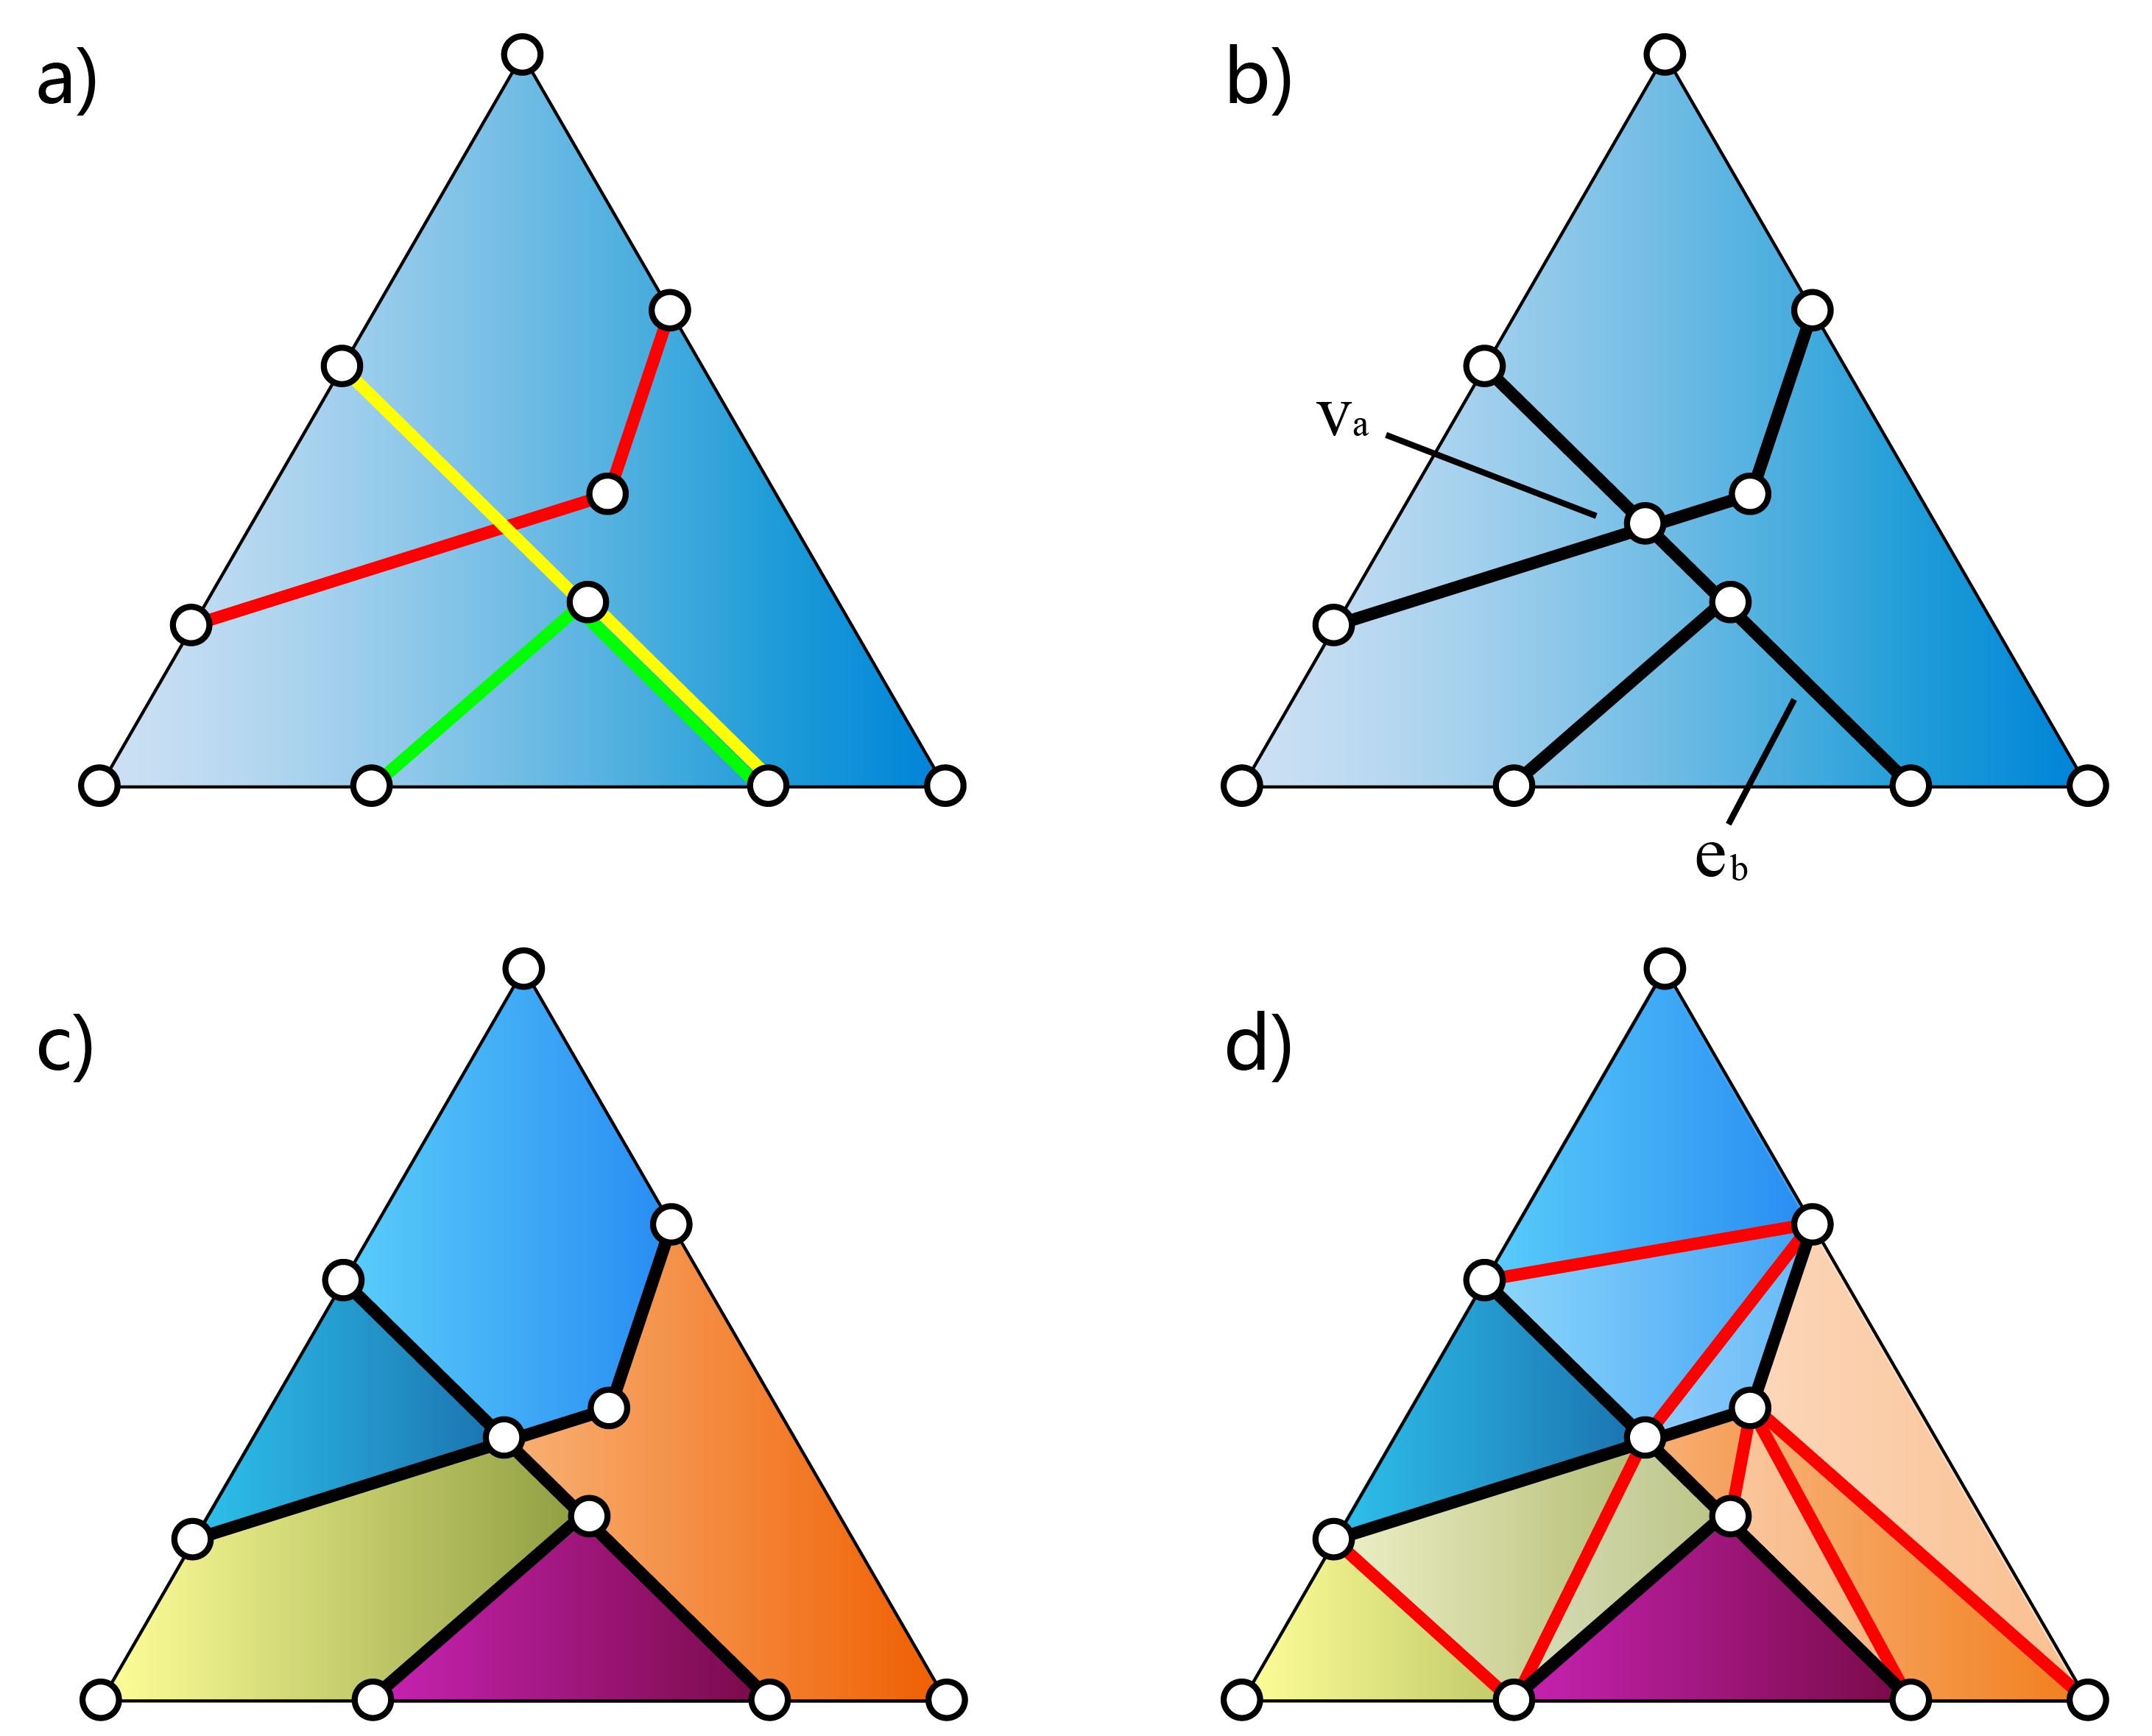
\includegraphics[width=3.5in]{boolean-04}
\caption{a) Different colors indicate the intersections are from different meshes. The blue intersections and the red ones intersect at a point. Also, the yellow intersections overlap with the red ones. b) After refinement, we introduce a new vertex $a$, and merge overlapping intersections into a new one $\mathcal{I}_b$. c) Our tessellation does not guarantee to obtain triangles. d) If triangulation is performed, new edges (gray ones) are introduced and we cannot give the precise plane-based representation for these new edges.}
\label{fig:iisect}
\end{figure}

To solve these problems, we first perform intersection refinement to eliminate any crossing or overlapping between intersections. After that, we perform conservative tessellation based on \emph{tess-graph}, ensuring unconditional topology correctness. An tess-graph is a graph-like description of intersections on a certain face. The word `conservative` means we . This is because if triangles are required, we need construct new bounding planes for these new triangles, which violating our principle of no geometry construction (Fig. \ref{fig:iisect}d).

\subsection{Intersection Refinement}


The intersection vertices are not only introduced by intersection between an edge and a triangle, but also introduced by intersections of three triangles. In order to find all intersection vertices, it is not enough by only triangle-triangle intersection tests. To make tessellation easier and more robust, we have to refine these intersections and resolve the intersections between intersections.

Intersection refinement is performed in a local scope. For each intersecting face $t$ from mesh $M_t$, we collect all intersections on $t$ as set $\bm{\Gamma}(t)$
%$\bm{\Gamma}(t)=\{\bm{\mathcal{I}}_{t}^i, i=0,1,2,...\}\cup\{\bm{\mathcal{I}}_{t}^{\bm{e}_i},i=0,1,2\}$
and refine them together. For simpler processing, we also include the three edges of $t$ into $\bm{\Gamma}(t)$, since edges also participate in tessellation. In $\bm{\Gamma}(t)$, edges are represented as PBI. The neighborhood components of edges are set as $None$ because they do not have a neighborhood edge or face. Other PBI-rep components can be determined by the P-reps of edges. The refinement on $\bm{\Gamma}(t)$ is done using only plane-based geometry predicates by the following three steps:

\vspace{0.5em}
\noindent \textbf{Coincidence elimination}~~~~
We merge coincidence intersections which have the same end points. Intersections are undirected so intersections with inverse end points are also coincident. The PBI-rep of the new intersection is inherited from either of the old one's except the neighborhood component. The new neighborhood is the combination of the merged ones', meaning the intersection has two (or more) neighborhoods.

\begin{wrapfigure}{r}[0in]{0in}
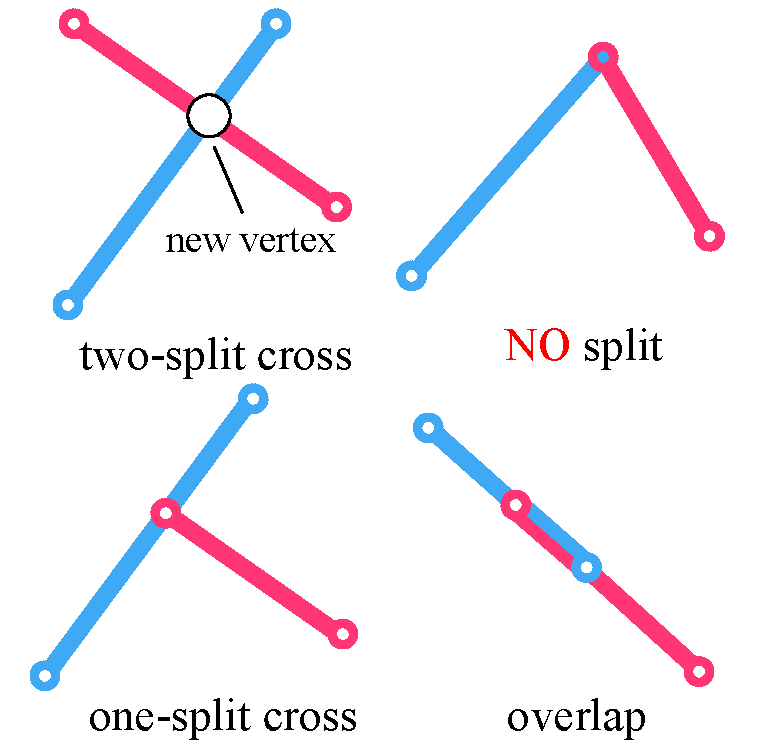
\includegraphics[width=1.7 in]{resolve}
%\caption{Plane-based representation of triangle}
\end{wrapfigure}
\vspace{0.5em}
\noindent \textbf{Cross and overlap resolving}~~~~
After the process of two previous steps, there are no overlapping intersections in $\bm{\Gamma}(t)$. We check whether any pair of intersections cross or overlap (collinear) each other. The definition of \emph{cross} does not include the situation that two intersections share end points, since no splitting is required in this situation. When there is crossing or overlapping, at least one of the intersections have to be split. Because one intersection may may 'touch' more than one other intersections, the splitting is deferred until all splitting points are found. The subroutine linear order of points (\S\ref{sec:substrates}) is used to sort these splitting points along the splitting intersection. The PBI-reps of split segments inherit their father's except the third component which identifies the end points.

\vspace{0.5em}
\noindent \textbf{Coincidence elimination (again)}~~~~
Unfortunately, the overlap resolving may bring new coincident intersections. Therefore the first step is run again in the final step.

%\vspace{0.5em}
%There is one more thing that we give intersections generated (by merging or splitting) from the PBI-reps of edges  the positive directions. That means all intersections lies on triangle edges have a positive direction. Direction is defined by the direction of edge the intersection lies on.

\subsection{Tessellation by Tess-Graph}
\label{sec:tess}



So far, intersections are only independent data that store the coordinates and neighbouring information. To perform tessellation and extract subfaces, we need to organize them to reveal the topology. We use tess-graph for this purpose. A tess-graph is the graph description of the tessellated face topology. For each face to be tessellated, we construct a tess-graph according to the refined intersections. Nodes of tess-graph represent end points of intersections and undirectional connections between nodes represent intersections. The construction of tess-graph is straightforward and the reader will not have problem filling the details.


After we have tess-graph, we tessellate face and extract subfaces according to it. This is done by extract valid loops on tess-graph. A valid loop that corresponds to a subface must satisfy two criterions: 1) the direction of loops should be coherent with the face normal, and 2) consecutive connections on the loop should be adjacent by circular order. Each valid loop corresponds to a intersection-free face. After we find out all valid loops on tess-graph, we finish tessellating the corresponding face. To facilitate the later process, we also store neighborhood information into the edges of the new faces. Because the edges of new faces are generated from intersections, the neighborhood information of the edges is inherent from the corresponding intersections.

\begin{figure}[t]
\centering
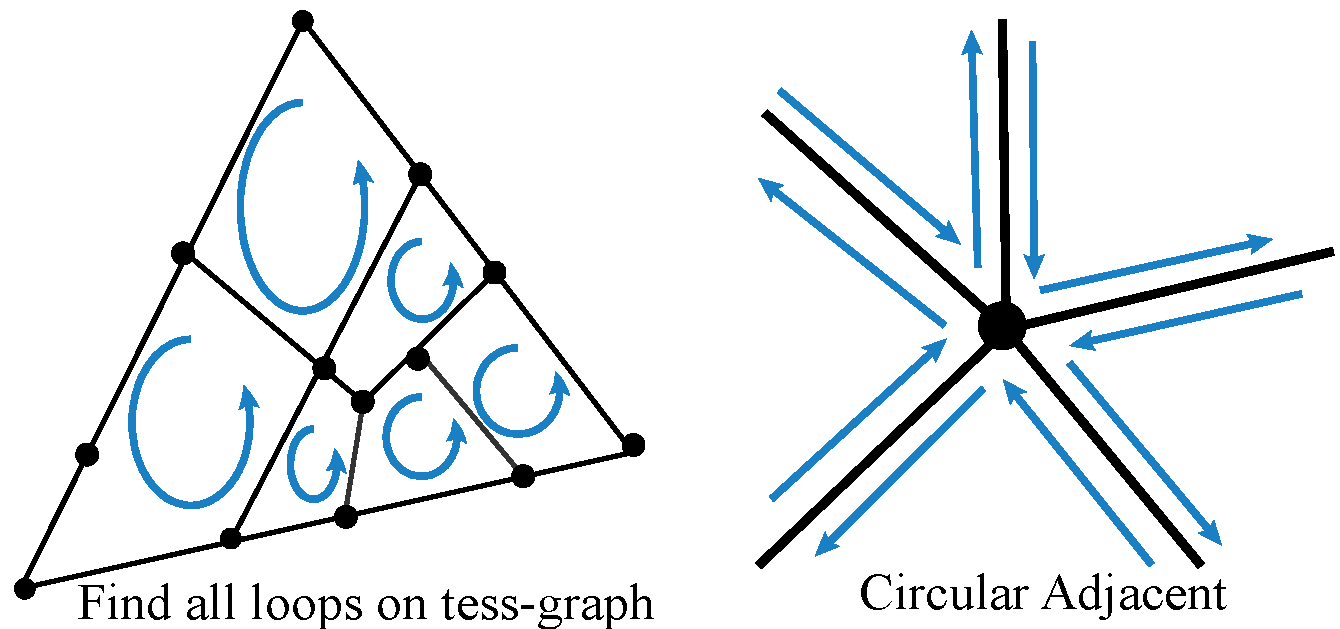
\includegraphics[width=3in]{circularadj}
\caption{\emph{Left}: we find all valid loops on tess-graph to tesselate a triangle. The direction of loops have to be coherent with the triangle normal (assume the normal points to the outside of paper). \emph{Right}: each circular adjacent edge pair is an angle of the tessellated polygon.}
\label{fig:cadj}
\end{figure}

When all faces are tessellated, meshes are intersection-free. We further attach the PBI-reps of intersections to the edges generated from tess-graph connections which corresponds to an intersection. Finally, we get the intersection-free hybrid meshes, with some edges contains neighborhood information which indicates there are intersections between meshes.

%In our implementation, we find that it is not easy to check whether the loop direction is coherent with face normal by plane-based geometry.

%First, We classify connections of tess-graph into two types: connections on face boundaries as \emph{boundary connections} and connections inside face as \emph{inner connections} by the whether they have positive directions. In the view of halfedge, inner connections represent two opposite halfedges but boundary connections represent only one. We add an attribute for each connection to identify their directions, and thus we get a directed version of Tess-graph. A sub-face is a halfedge loop on the directed Tess-graph. Extracting faces are process of searching for valid loops which meet certain geometry constraints. After all faces are extracted, all halfedges of directed Tess-graph should be used

%There two geometry constraints for valid loops. Second, consecutive connections on the loop should be adjacent by circular order {\color{red}{Fig.?}}. To meet these constraints, we sort the halfedges counter-clockwise for each nodes with more than two halfedges starting from them. This is implemented by using the divide-and-conquer framework of quick sort. During each recursion, we pick a random halfedge and split the rest into two sets according to the sign of two-line-on-plane comparison. To make the results of two-line-on-plane comparisons coherent, we assume that for each halfedge $h_i$, the normal directions of its plane-rep, denoted as $\vec{n}(h_i)$, meets the following criterion:
%\begin{equation}
%(\vec{n}(h_i) \times \vec{n}_0) \cdot \vec{l}(h_i) > 0,
%\end{equation}
%where $\vec{n}_0$ is the normal of the face, and $\vec{l}(h_i)$ is the direction of $h_i$. The plane-rep of halfedge can be inherited from the corresponding connections from the undirected Tess-graph. Since we {\color{red}{guarantee that each connection has a plane-rep //need insert//}}, sorting can be exactly and fast performed. After connections are sorted in each nodes, we can know which connections are adjacent and what is the right direction during the loop search.


\section{Face Classification}

\label{sec:classification}
We traverse each face in the intersection-free meshes, and classify which one belongs to the final mesh. Classification is done by evaluating the indicator vector of each face. The basic idea of our classification method is to utilize the space coherence of face indicator vectors to reuse the classification results. Because we store the PBI-reps which contains neighborhood information in the edges which intersect other meshes, the search space of point-in-polyhedron test is limited to only a few faces, which makes the indicator computation very fast. Also, by using P-reps, our classification method can deal with any degenerate cases.


The space coherence of indicator vectors means neighboring faces could share the same indicator vector, or most components of indicator vectors. Therefore, we start from a seed face $\bm{s}_0$ with its indicator vector $\bm{\Lambda}(\bm{s}_0)$ known, and propagate to other faces in a flood-filling manner. The trace of indicator propagation is:
\begin{equation}
\label{eq:trace}
\bm{s}_0\to \bm{s}_1\to \bm{s}_2\to \bm{s}_3\to ...
\end{equation}


Our hybrid meshes facilitate this process by accelerating the indicator propagation. Given adjacent faces $\bm{s}_1$ and $\bm{s}_2$, it is straightforward to know whether $\bm{\Lambda}(\bm{s}_1)$ and $\bm{\Lambda}(\bm{s}_2)$ are different. The two indicator vectors are the same unless the shared edge $\bm{e}_{12}$ lies on the boundary of some other meshes, which means there is neighborhood information, say, $\bm{\mathcal{N}(\bm{e}_{12})} = \{(P_k, \mathcal{N}_k)\}$, stored on $\bm{e}_{12}$. The neighborhood information indicates which components of indicator vector differ between $\bm{s}_1$ and $\bm{s}_2$.
 \iffalse
 Namely, for a certain indicator $\lambda_k$ of $\bm{s}_1$ and $\bm{s}_2$, it always stands:
\begin{equation}
\label{eq:eq1}
{\lambda_k}(\bm{s}_1) = {\lambda_k}(\bm{s}_2),\ \ \  \mbox{if }\mathcal{N}_k(\bm{\mathcal{I}}(e_{12}))= 0.
\end{equation}
\fi
If there is a neighborhood $(P_k, \mathcal{N}_k) \in \bm{\mathcal{N}}(\bm{\bm{e}_{12}})$, the $k^{th}$ indicators $\lambda_k(\bm{s}_1)$ and $\lambda_k(\bm{s}_2)$ can be computed efficiently and exactly according to $\mathcal{N}_k$ (\S\ref{sec:propagation}). We outline our classification method in Algorithm \ref{code:floodfill}.


\begin{algorithm}
\caption{Fast Face Classification}
\label{code:floodfill}
\textbf{Input: } Intersection-free hybrid meshes, boolean function $f$

\textbf{Output: } Classification $f(\bm{\Lambda}(\bm{s}_i))$ for all faces $\bm{s}_i$


\begin{algorithmic}[1]
\State Select a proper seed face $\bm{s}_0$
\State Compute the seed indicator vector $\boldsymbol{\Lambda}(\bm{s}_0)$
\State \Call{propagate} { $\bm{s}_0$ , $\boldsymbol{\Lambda}(\bm{s}_0)$}
\State
\Function{propagate}{ $\bm{s}$ , $\boldsymbol{\Lambda}(\bm{s})$}
    \State Compute $f(\boldsymbol{\Lambda}(\bm{s}))$
    \For {each neighboring face $\bm{s}_{s, i}$}
        \If {$\bm{s}_i$ has been classified}
            \State continue
        \EndIf
        \If {there are PBI-reps ${\bm{\mathcal{I}}}_k$ on $\bm{e}(\bm{s}_{s, i}, s)$}
            \State compute $\boldsymbol{\Lambda}(\bm{s}_{s, i})$ by $\boldsymbol{\Lambda}(\bm{s})$ and ${\bm{\mathcal{I}}}_k$
            \State \Call{propagate} { $\bm{s}_{s, i}$ , $\boldsymbol{\Lambda}(\bm{s}_{s, i})$}
        \Else
            \State \Call{propagate} { $\bm{s}_{s, i}$ , $\boldsymbol{\Lambda}(\bm{s})$}
        \EndIf
    \EndFor
\EndFunction
\end{algorithmic}
\end{algorithm}

\iffalse
\subsection{Precise Seed Generation}

Our classification method starts from computing the seed indicator vector using point-in-polyhedron test \cite{ogayar2005point}. Conventionally, the barycenter of the face is used for the test to compute the indicator vector of the whole face. This is because the whole face is classified as a whole, and every inner point will have the same indicator vector. However, the coordinates of the inner points cannot be exactly represented by float point numbers, which may lead to wrong predicates, especially when it is an on-boundary case. Therefore, we use the original vertices, whose exact coordinates are known, for point-in-polyhedron test. For this reason, only tessellated faces with at least one original vertex can be the seed face. The point-in-polyhedron test is guaranteed to be exact. On the other hand, efficiency is not so important as there will not be many such tests. If ray-trace algorithms (e.g., \cite{frisken2002simple}) are used, the octree constructed during space division can be used for acceleration \cite{havran1999summary}.

However, using point on the boundary instead of an inner one has another problem. Given a face $\bm{s}$ (may not be triangle) and one of its vertex $v_b^i(\bm{s})$, the vertex indicator $\boldsymbol{\Lambda}(v_{i}(\bm{s}), P_k)$ may cause ambiguity to deduce the face indicator $\boldsymbol{\Lambda}(s, P_k)$. In {\color{red}{Fig. ?}}, $\boldsymbol{\Lambda}(v_b^1(\bm{s}), P_k) = on$, then $\boldsymbol{\Lambda}(s, P_k)$ can be any of the four conditions. We solve this problem by trying other vertices in $\bm{s}$ for ambiguous indicators. If all vertices indicators are $on$ and the ambiguity cannot be resolved, the current face is not proper for being the seed and we select a new one instead.

\fi

\subsection{Indicator Propagation}
\label{sec:propagation}


Meshes consist of vertices, edges and faces. Classification is required to perform on the face level. However, polyhedron in-out test is performed based on points. Gaps exist between the them. Conventionally, face barycenter is used to compute the indicator of the whole face. This is because in intersection-free meshes, face is classified as a whole, and every face inner point will have the same indicator as the face's. However, the computation of inner point coordinates requires geometry construction, which introduces errors without exact arithmetic. Therefore, we use the vertices instead, whose exact representations are known, for indicator computation.

\begin{wrapfigure}{r}[0in]{0in}
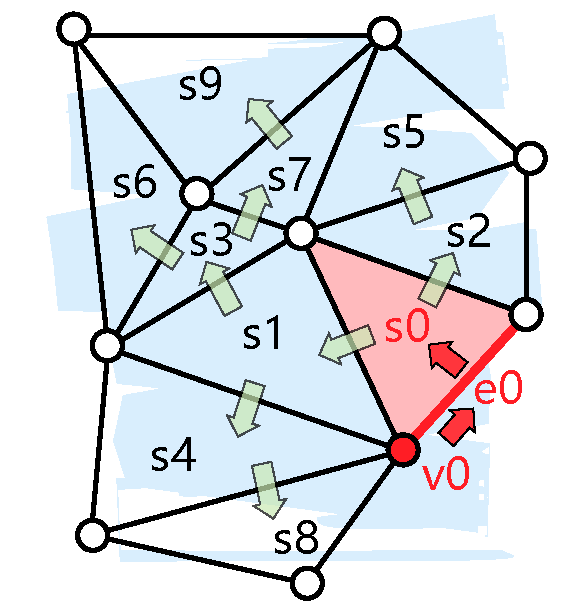
\includegraphics[width=1.3 in]{propagate}
\end{wrapfigure}


%For example, given a face $\bm{s}$ and one of its vertex $v^i(\bm{s})$, if $\lambda_k(v^i(\bm{s}))=on$, $\lambda_k(\bm{s})$ can be any of $on$, $in$ or $out$ (see {\color{red}{Fig. ?}})
However, there are two gaps between face indicator and vertex indicator. First, the indicator of vertex does not always equal to indicator of face. Second, face indicator has two conditions in $on$ case---$same$ and $oppo$, because the face has its orientation.

To overcome the gaps, we discuss our indicator trace (\ref{eq:trace}) in finer granularity. In the beginning, we start from a seed vertex $\bm{v}_0$ on seed face $\bm{s}_0$. We assume indicator vector $\bm{\Lambda}(\bm{v}_0)$ is known. Then we use $\bm{\Lambda}(\bm{v}_0)$ to compute $\bm{\Lambda}(\bm{s}_0)$. In addition, we add the edge layer into the trace. Then it changes to:
\begin{equation}
\bm{v}_0\to \bm{e}_0\to \bm{s}_0\to (\bm{e}_1)\to \bm{s}_1\to (\bm{e}_2)\to \bm{s}_2\to ...
\end{equation}
, where $\bm{v}, \bm{e}$ means vertex and edge respectively. The bracket here means propagating to edge is optional because if the edge does not contain neighborhood information, the indicators on the two side are the same and we do not need to propagate to the edge. We find that there are three kinds of basic operations in the trace: $\bm{v}_{\bm{e}}\to \bm{e}$, $\bm{e}_{\bm{s}}\to \bm{s}$ and $\bm{s}\to \bm{e}_{\bm{s}}$, where $\bm{v}_{\bm{e}}$ means the end point of $\bm{e}$, and $\bm{e}_{\bm{s}}$ means the edge of $\bm{s}$.

\begin{figure}[t]
\centering
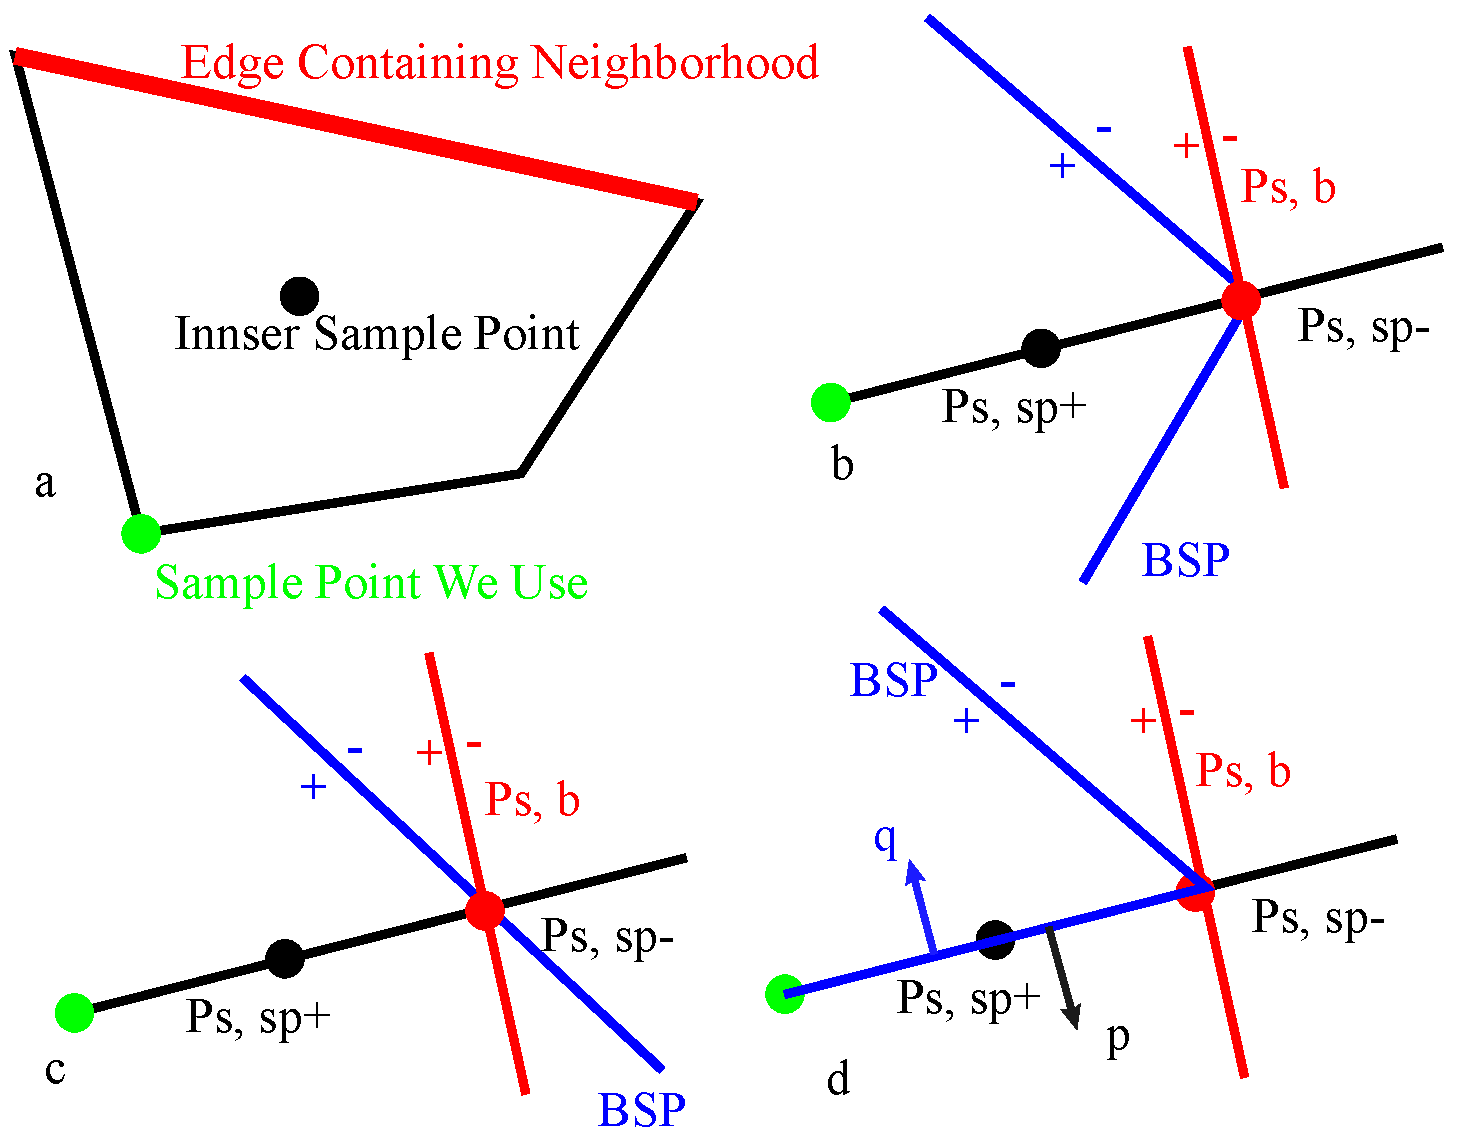
\includegraphics[width=3in]{bsps}
\caption{a) Because we cannot use inner sample point includes geometry construction, we choose the vertices (green one) instead to compute the face indicator. b-d): Different situations of classification. The simple structure of neighborhood BSP guarantees the same classification result of the points on $\bm{p}_{\bm{s}, sp}^+$. In \emph{a}, the BSP contains two half-planes because it is constructed from two neighborhood faces. In \emph{d}, the classification result is $on$ so we need to determine the orientation by the normal of half-plane $q$ and the face $p$. In this condition, the indicator should be $oppo$ since $p$ and $q$ are opposite.}
\label{fig:bsps}
\end{figure}

Given the partial order $on \succ in$ and $on \succ out$, our key observation is that the following relation always stands for indicators:
\begin{equation}
\label{eq:porder}
\lambda_k(\bm{v}_{\bm{e}_{\bm{s}}}) \succeq \lambda_k(\bm{e}_{\bm{s}}) \succeq \lambda_k(\bm{s})
\end{equation}
, where $\lambda_k(x)$ means the indicator of $x$ against a certain primitive $M_k$. This relation can be inferred from continuous space assumption and the definition of intersection-free mesh. It tells us when we perform $\bm{v}_{\bm{e}}\to \bm{e}$ and $\bm{e}_{\bm{s}}\to \bm{s}$, we decide whether the $on$ indicator changes to $in$ or $out$ or remains $on$. When we perform $\bm{s}\to \bm{e}_{\bm{s}}$, we decide whether $in$ and $out$ indicators change to $on$. In addition, considering the orientation of face, we also need to figure out whether the $on$ indicators changes to $same$ or $oppo$ during $\bm{e}_{\bm{s}}\to \bm{s}$ operation.

\vspace{0.5em}
\noindent\textbf{$\bm{s\to \bm{e}_{\bm{s}}}$}~~~~ We need to find which indicators change to $on$. We known when $\lambda_k(\bm{e}_{\bm{s}})=on$, there will be neighborhood information related to mesh $M_k$ stored on $\bm{e}_{\bm{s}}$. Therefore, in this operation, all we need is to iterate over neighborhoods of $\bm{e}_{\bm{s}}$ and change corresponding indicators to $on$.


\vspace{0.5em}
\noindent\textbf{$\bm{\bm{e}_{\bm{s}}\to \bm{s}}$}~~~~From eq. \ref{eq:porder}, we know if $\lambda_k(\bm{e}_{\bm{s}}) \neq on$, then $\lambda_k(\bm{e}_{\bm{s}})=\lambda_k(\bm{s})$. On the other hand, when $\lambda_k(\bm{e}_{\bm{s}}) = on$, we figure out $\lambda_k(\bm{s})$ using neighborhood information related to $M_k$. We know the corresponding neighborhood $\mathcal{N}_k$ and can be either a triangle face or an edge from mesh $M_k$. If $\mathcal{N}_k$ is a face, we can build a trivial BSP \cite{thibault1987set} using the face on the space near $\bm{e}_{\bm{s}}$. If $\mathcal{N}_k$ is an edge, we can still build BSP using the faces adjacent to $\bm{e}_{\bm{s}}$. In both cases, the BSP can be used to compute $\lambda_k(\bm{s})$ if we can sample a point from $\bm{s}$ that near $\bm{e}_{\bm{s}}$. Unfortunately, we cannot guarantee to find such a point with precise coordinates.

We find that the BSP constructed from edge neighborhood is so simple that indicators $\lambda_k$ of all points on the half plane $\bm{p}_{\bm{s}, sp}^+$ are the same. Here $\bm{p}_{\bm{s}, sp}^+$ is half of the supporting plane of $\bm{s}$ that on the positive side of bounding plane $\bm{p}_{\bm{s}, b}^{\bm{e}_{\bm{s}}}$ (Fig. \ref{fig:bsps}). Since $\bm{p}_{\bm{s}, sp}^+ \cap \bm{s} \neq \varnothing$, we can compute $\lambda_k(\bm{s})$ by figuring out $\lambda_k(\bm{v}_x)$, where $\bm{v}_x \in \bm{p}_{\bm{s}, sp}^+$. For polygons, there is at least one vertex on $\bm{p}_{\bm{s}, sp}^+$, whose exact coordinates are known. Therefore that vertex is used as the $v_x$. Also, if we assign each BSP splitting plane a normal by the normal of triangle it contains, we can use it to decide the orientation ($same$ or $oppo$) when $\bm{v}_x$ is on a splitting plane, which means $\lambda_k(\bm{s})=on$.

\vspace{0.5em}
\begin{wrapfigure}{r}[0in]{0in}
 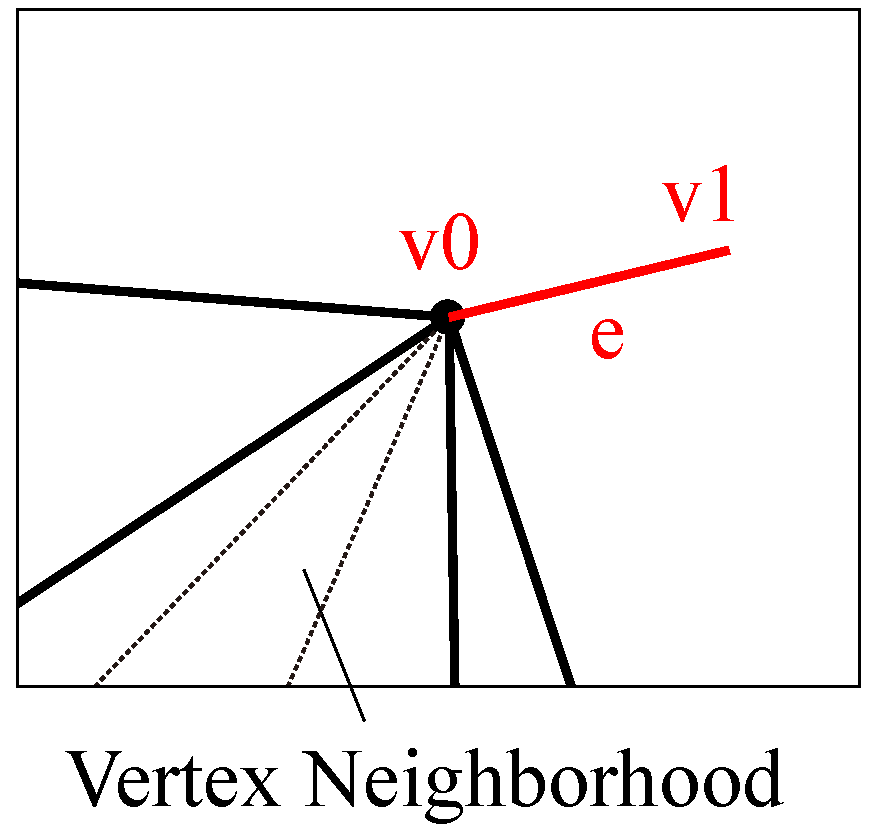
\includegraphics[width=1.3 in]{vneighbor}
\end{wrapfigure}
\noindent\textbf{$\bm{\bm{v}_{\bm{e}}\to e}$}~~~~ While this is yet another propagation from low dimension to high dimension, there is no neighborhood information stored on vertex. If $\lambda_k(\bm{v}_{\bm{e}})=on$, we first check whether $\lambda_k(\bm{e}) = on$ by checking the neighborhood component of the intersection on $\bm{e}$. If not, we need to find where $\bm{v}_{\bm{e}}$ lies on the surface of $M_k$ and determine the neighborhood of $\bm{v}_{\bm{e}}$. In most cases, it is straightforward since coincident vertices among different intersection-free meshes are shared (see \S\ref{sec:esubroutine} for exception discussion). The neighborhood may be a vertex, an edge or a face. After computing the neighborhood, the same BSP-based classification method is used as in ${\bm{e}_{\bm{s}}\to \bm{s}}$ to determine the high dimension indicator $\lambda_k(\bm{e})$. We use the other end point of $\bm{e}$ to be the sample point for the BSP classification.


\subsection{Acceleration by Caching}
\label{sec:acc}
If the CSG tree is large with hundreds of primitive nodes, computing $\lambda_f(\bm{s}_i)$ from $\boldsymbol{\Lambda}(\bm{s}_i)$ for every face $\bm{s}_i$ can be costly. Thanks to the indicator space coherence, we can save the computation time by caching the evaluation result $f(\boldsymbol{\Lambda}(\bm{s}_i))$ during flood-filling.

The basic cache strategy is to cache final result, that is, the value of $\lambda_f(\bm{s}_i)$. We know indicator vector will not change if there is no intersections on the edge during propagation. That means the final classification $\lambda_f(\bm{s}_i)$ will not change, too. Thus, those faces sharing the same indicator vector can be classified as a whole.

Also, we can perform intermediate results cache. We noticed that the boolean expression can be simplified if some components of $\boldsymbol{\Lambda}(\bm{s}_i)$ is fixed. For example, assume we have a boolean expression $f = P_1\cup (P_2\cap P_3-P_4)$. Given the values of two indicators $\lambda_1(\bm{s}_i)=out$, $\lambda_2(\bm{s}_i)=in$, the expression can be rewritten as $f(\lambda_1=out, \lambda_2=in)=out\cup (in\cap P_3-P_4)$. Using the combination rules we can simplify the expression as $f(\lambda_1=out, \lambda_2=in)=P_3-P_4$. This fact is important because for a large CSG, a certain primitive (denoted as $M_k$) often intersects with only a few other meshes $\Theta(P_k)= \{P_{n_1}, P_{n_2}, \cdots, P_{n_x}\}$. That means all the faces in $M_k$ has the same indicators $\lambda_{i}, P_{i} \notin \Theta(P_k)$. Therefore, we can first determine these fixed indicators and simplify the boolean function, and then use simplified one to compute the final indicator for each faces in $M_k$.



\iffalse
\subsection{Tessellating on Classification}
We find for a CSG with many meshes, a large percentage of intersections are invalid (see \S\ref{sec:degenerate} for 'invalid'). Tessellation according to these invalid intersections is not necessary. To avoid unnecessary tessellation, we can give an early prediction of which intersections are invalid by intersections information of faces, but have to embed the tessellation stage into the classification stage, which we call it 'tessellating on classification'.

In most situations, a certain faces $\bm{s}$ only intersect with a few other meshes $\Theta(\bm{s})$. We can use the same cache strategy in \S\ref{sec:acc} to shrink the original CSG into a smaller one by the common indicators of $\{P_i\}\backslash\Theta(\bm{s})$, where $\{P_i\}$ means all the primitive meshes. After the shrinking, the primitive meshes of the CSG must be from $\Theta(\bm{s})$. If any mesh in $\Theta(\bm{s})$ does not appear in the shrinked CSG, it means the indicator of that mesh does not change the classification result, which in another word, intersections on $\bm{s}$ from that mesh are invalid and do not affect the classification of any subfaces of $\bm{s}$. If the shrinked CSG is trivial which does not contain any primitives, it means $\bm{s}$ does not need tessellation. In this way, we save the computation time, and simplify the topology of the final result mesh. Because we can only shrink the CSG for $\bm{s}$ when we classify it---before that the indicators of meshes from $\{P_i\}\backslash\Theta(\bm{s})$ are not known---we do not perform tessellation until we do the classification.



\subsection{Implementation}

\label{sec:individual}

Feito et. al. \cite{feito2013fast} had noticed that intersection neighborhood can be used for fast classification of faces around that intersection. According to their method, faces adjacent to intersection have neighbors from other primitive(\bm{s}) that define the position and orientation for each other, by which the indicators are determined. However, Feito et. al. did not give detail description of how to implement an exact and robust classification. Their implementation of using vertex coordinates might misclassify faces by numeric errors and fail in degenerate cases. Because geometry connectivity is used, local misclassification can be spread to the neighborhoods, leading to errors in wide ranges.

We develop an classification method that is unconditionally robust and exact based on the idea of using intersection neighborhood information. The neighborhood information is stored in the context component of I-reps during previous stages . In the following, we discuss the conditions that the face to be classified is a triangle. If the face is not a triangle, we select a triangle slice of the face instead, as the whole face is guaranteed to be classified together. Note that the chosen slice should contain the edge where the I-reps lie, by which we compute the new indicators.

Given a face $t_i$ to be classified and an I-rep $\boldsymbol\Gamma$ of intersection on one of $t_i$'s edge, we denote the three corners it as $\bm{v}_{b*}^{0}(t_i), \bm{v}_{b*}^{1}(t_i), \bm{v}_b^2(t_i),$ where the subscript $*$ means the vertices are on the edge where $\boldsymbol\Gamma$ lies. We also denote the context component of $\boldsymbol\Gamma$ as $C_{P_h \backslash P_j}$, meaning $t_i$ is from primitive $M_j$ and intersects primitive $M_h$. From previous discussion (section \ref{sec:ir}){\color{red}{may be more than one}}, we know there are two types of intersection context---face neighborhood and edge neighborhood. In both conditions, the one or two faces involving in the context split the space into two in and out space by its (their) orientation(\bm{s}). We will see that under such division (denoted as $\boldsymbol{D}(C_{P_h \backslash P_j})$), we can compute $\lambda(t_i, P_j)$ exactly.

Since the faces involving in $C_{P_h \backslash P_j}$ is part of primitive $M_j$, the space division $\boldsymbol{D}(C_{P_h \backslash P_j})$ is homogeneous with the space division by $M_j$ in neighborhood of $\bm{\mathcal{I}}$. The basic idea is to choose one point $\bm{v}_x(t_i)$ on $t_i$ close enough to $\bm{\mathcal{I}}$ to compute $\lambda(\bm{v}_x(t_i), P_j)$, and then compute $\lambda(t_i, P_j)$ accordingly. However, the problem is that we cannot find such a $\bm{v}_x(t_i)$ that can be represented exactly, which means robust classification cannot be performed. Fortunately, we observe that we can choose $\bm{v}_b^2(t_i)$, which is not so close to $\bm{\mathcal{I}}$ instead. To illustrate, assume there is another point $\bm{v}_{x'}(t_i)$ inside of $t_i$ that is very close to $\bm{v}_b^2(t_i)$ ({\color{red}{Fig. x}}). Because all inner points of $t_i$ have the same indicator, $\lambda(\bm{v}_x(t_i), P_j) = \lambda(\bm{v}_{x'}(t_i), P_j)$. On the other hand, we find that $\lambda(\bm{v}_{x'}(t_i), P_j)$ and $\lambda(\bm{v}_b^2(t_i), P_j)$ are always equal under division $\boldsymbol{D}(C_{P_h \backslash P_j})$ ({\color{red}{see Appendix \ref{app:profind}}}). Therefore, $\lambda(\bm{v}_b^2(t_i), P_j)$ is equal to $\lambda(\bm{v}_x(t_i), P_j)$ under $\boldsymbol{D}(C_{P_h \backslash P_j})$, and are coherent with $\lambda(t_i, P_j)$ under the division of whole primitive $M_j$. One additional thing is that when $\lambda(\bm{v}_2(t_i), P_j)=on$, then $\lambda(t_i, P_j)$ can be either $same$ or $oppo$. The normal orientation test have to be performed to eliminate such ambiguity.

\fi

\section{Results and Discussion}


\begin{figure}[t]
\centering
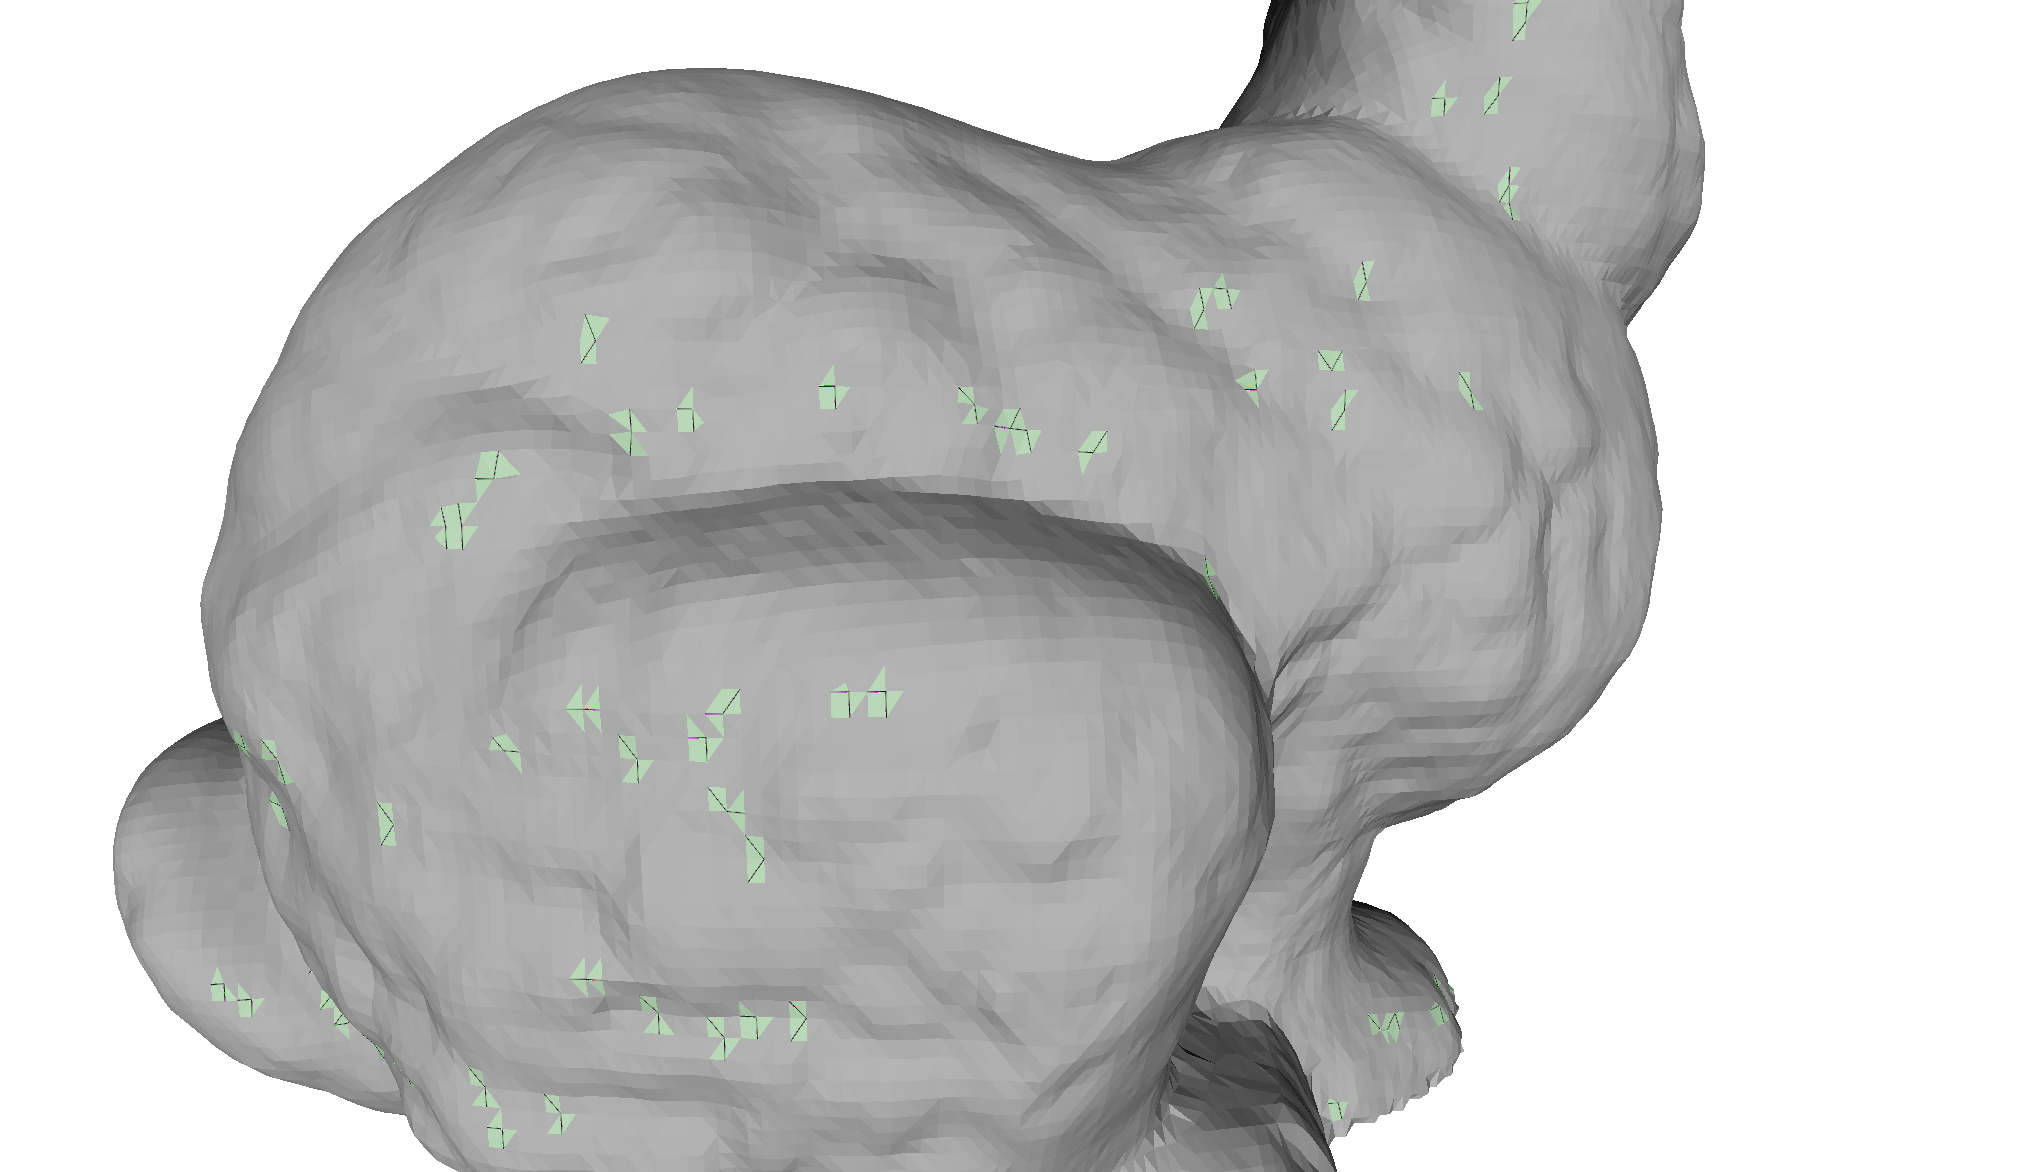
\includegraphics[width=3in]{perturb}
\caption{Even after perturbation, the self-union of \emph{bunny} under QuickCSG still suffers from topology problem. The green faces are boundary faces which indicating topology deficiencies.}
\label{fig:boundaryedge}
\end{figure}

\begin{figure}[t]
\centering
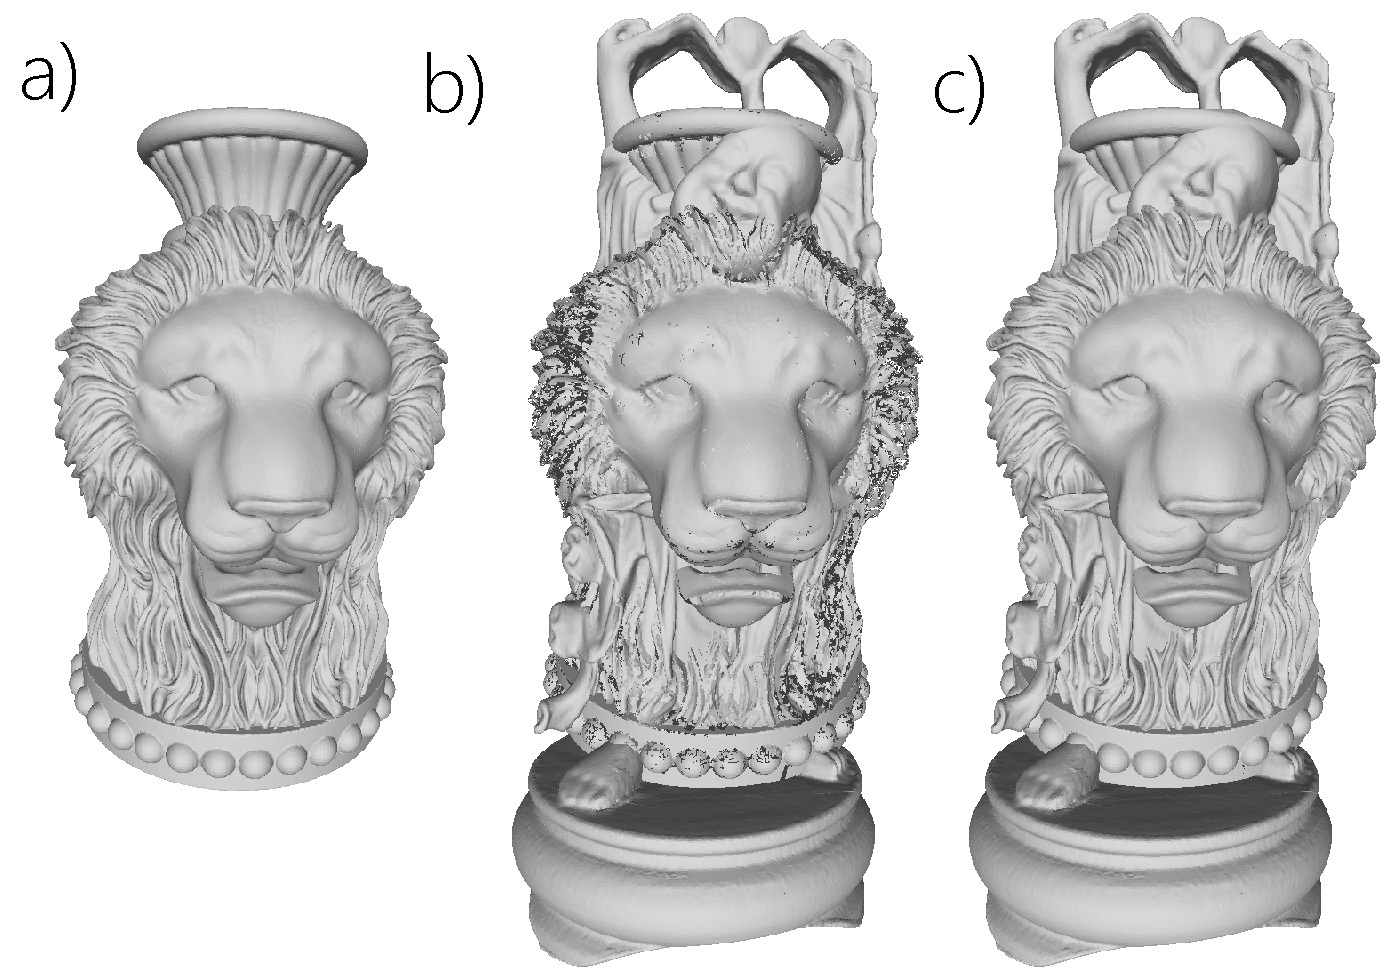
\includegraphics[width=3in]{buddalion}
\caption{ Different results from $Budda\cup Lion$: a) incorrect result by CGAL, b) incorrect result by Cork, and c) correct result by our method. }
\label{fig:buddalion}
\end{figure}

We implemented the proposed method in C++ and tested a series of models on a laptop with Intel Core i5 1.5GHz CPU and 8GB RAM. To prove both the efficiency and robustness, we perform boolean evaluation on various CSGs with different complexity.To show our advantage, we also compared our method with several previous works with available implementations, including CGAL \cite{cgal:hk-bonp3-15a}, Maya \cite{Maya2015,barki2015exact},"Cork" \cite{Cork}, "QuickCSG" \cite{douze2015quickcsg}, "Carve" \cite{Carve}, and online service of Campen and Kobbelt's plane-based method \cite{campen2010exact,WebBSP}.



\subsection{Robustness}



\begin{figure}[t]
\centering
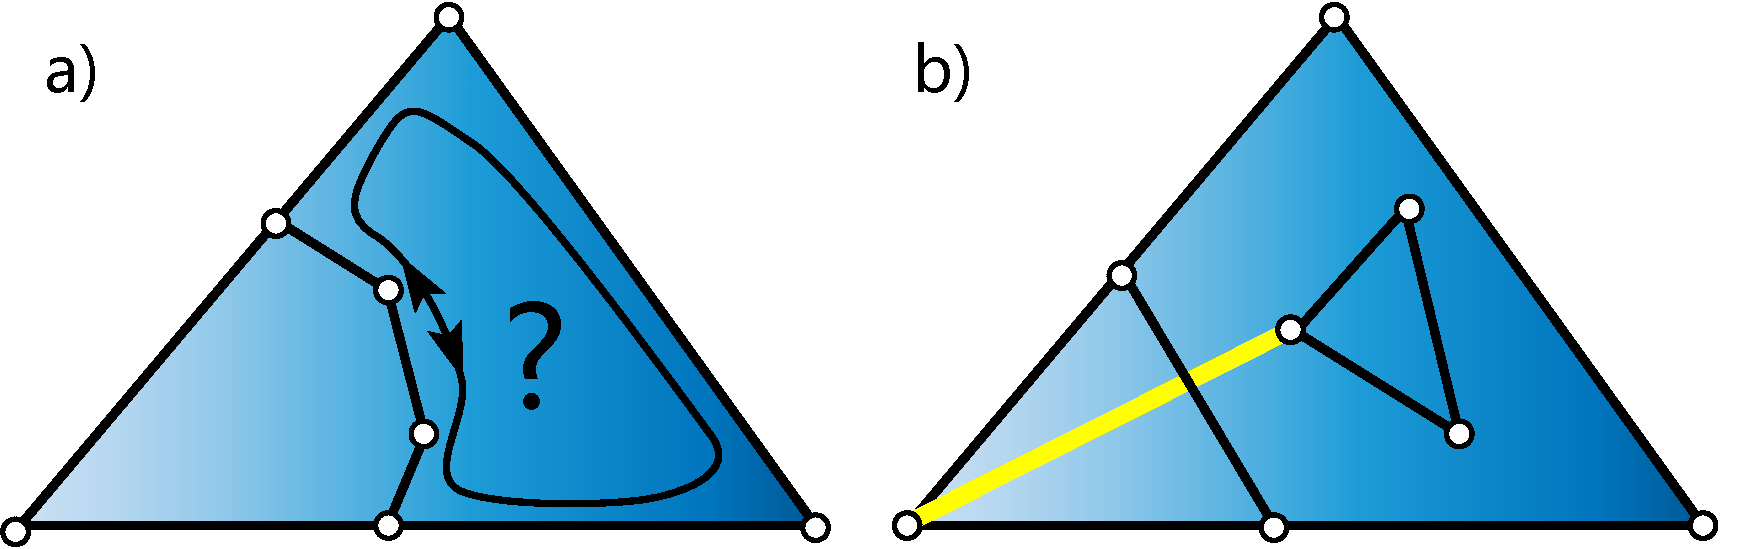
\includegraphics[width=3in]{dual}
\caption{a) We cannot easily figure out the correct orientation of the loop. b) When there are more than one connected component, we use auxiliary intersection (red line) to connect the two component. }
\label{fig:dual}
\end{figure}


\begin{table*}[ht]
\caption{Computation Time Statistics of Binary Boolean Operation (Seconds)}
\label{tab:performance}
\centering
\begin{tabular}{*{9}{c|}c}%*{4}{>{\centering\arraybackslash}p{35pt}}}
\hline
{No.} & {Model} & {Triangle Num. 1} & {Triangle Num. 2} &
CGAL & Maya & Cork & Carve & QuickCSG & Our Method
\\
\hline\hline
1 & Budda $\cup$ Lion & 1.08M & 400k & - & - & - & - & 3.44 & 6.88\\
2 & Dragon $\cup$ Bunny & 100k & 70k & - & - & - & - & 0.613 &1.70 \\
3 & Armadillo $\cup$ Armadillo2 & 150k & 150k & 487 & 15.4 & 7.00 & 189 & 0.746 & 1.62\\
4 & Horse $\cup$ Corpse & 145k & 499k & - & 38.6 & 12.6 & 1.52k & 0.630 & 1.00 \\
5 & Budda $\cup$ Budda2 & 1.08M & 1.08M & - & - & - & - & 4.84 & -\\
\hline
\end{tabular}
\begin{flushleft}

\end{flushleft}
\end{table*}

\begin{table*}[ht]
\caption{Computation Time Statistics of Large CSG Evaluation (Seconds)}
\label{tab:performance2}
\centering
\begin{tabular}{*{9}{c|}c}%*{4}{>{\centering\arraybackslash}p{35pt}}}
\hline
{No.} & {Model} & {Triangle Num.} & {Primitive Num.} &
CGAL & Maya & Cork & Carve & QuickCSG & Our Method
\\
\hline\hline
1 & Sprocket & 11k & 52 & 211 & ? & - & 4.26 & 0.132 & 0.804\\
2 & Ring \& Ball & 146k & 801 & - & ? & - & 187 & - & 62.6\\
3 & T1 & 80k & 50 & 1.00k & ? & 18.5 & 10.4 & 0.388 & 20.2\\
4 & T2 & 7k & 50 & 2.81k & ? & - & 16.0 & 0.804 & -\\
5 & H & 33k & 42 & - & ? & - & - & 2.22 & -\\
6 & Organic & 219k & 6 & - & ? & 14.3 & 63.1 & 0.580 & 2.75\\
%7 & 6 Budda & - & 43 & - & - & - & - & - & -\\
%8 & Serpent & - & 5 & - & - & - & - & - & -\\
\hline
\end{tabular}
\begin{flushleft}
\end{flushleft}
\end{table*}

\begin{table*}[ht]
\caption{Results of Self-Union Evaluation}
\label{tab:selfunion}
\centering
\begin{tabular}{*{8}{c|}c}%*{4}{>{\centering\arraybackslash}p{35pt}}}
\hline
{No.} & {Model} & {Face Num.} &
CGAL & Maya & Cork & Carve & QuickCSG  & Our Method
\\
\hline\hline
1 & Ball & 360  & \cmark & \cmark & \xmark & \cmark & \xmark & \cmark \\
2 & head & 2,716& \cmark & \cmark & \xmark & \cmark & \xmark  & \cmark\\
3 & Bunny & 69,666  & \xmark & \cmark & \xmark & \cmark & \xmark  & \cmark\\
4 & Dragon & 276,972 & \xmark & \xmark & \xmark & \xmark & \xmark  & \cmark \\
\hline
\end{tabular}
\begin{flushleft}
%~~~~~~~~~~~~~~~~~~~~~$^{*}$~~We perturb the model by 1e-6 to give QuickCSG the ability to partly solve coplanar cases.
\end{flushleft}
\end{table*}

Our method is unconditionally robust for regular set meshes. Even extreme degenerate cases will not cause invalid output. To prove that, we tested the self-union of several models and some CSG with coplanar faces. Table \ref{tab:selfunion} compares the difference between input meshes and result meshes by their face number. We find that our method always produces correct or at least near correct results. The slightly deviation of our result from the original one is caused by self-intersection in the original models. QuickCSG and Cork failed in all cases, because they cannot deal with coplanar faces. By perturb one of the operant, the results of QuickCSG are visually OK. However, the topology of their results is messy. We can see hundreds of boundary faces on their results which do not exist in the original model (Fig. \ref{fig:boundaryedge}).


\subsection{Performance}
\vspace{0.5em}
\noindent\textbf{Binary boolean operations}~~~~
The most common situation of CSG evaluation is to perform boolean operations one by one, since many designers are used to modify models progressively. While our method can evaluate multiple boolean operations once for all, we also compared the performance of binary boolean operations to prove the efficiency. Table \ref{tab:performance} shows the evaluation time of different methods. We can clearly see our method is very fast that is only twice as slower than the fastest non-robust QuickCSG. Other robust methods such as Maya and CGAL are much slower because both of them use the arbitrary precision arithmetic. Moreover, these robust methods have very strict requirements on the inputs and fragile with topology deficiencies such as boundary edges or self-intersection. On the contrary, our   We also noticed that in (some) very large CSGs, most time is spent on octree construction in our method. It means other stages which involve plane-based geometry take only a small percentage of time, proving the efficiency of our plane-based geometry.


\vspace{0.5em}
\noindent\textbf{CSGs with large number of meshes}~~~~
To identify the ability of evaluating large CSG, we also test some CSG with tens or hundreds of meshes. Maya and CGAL cannot perform multiple boolean operations, so we can only give the comparison of incremental boolean evaluation for these methods. We see that the computation time of robust methods like CGAL and Maya grows rapidly when the number of meshes grows. On the other hand, our method keeps good performance while stay robust. During our experiments, we noticed Maya gives the correct results in the first few boolean operations, but failed in the later ones. It proves a disadvantage of incremental boolean operation methods: if it cannot guarantee exactness, it will accumulate numerical errors which affects the algorithm stability.


\begin{figure*}[!t]
\centering
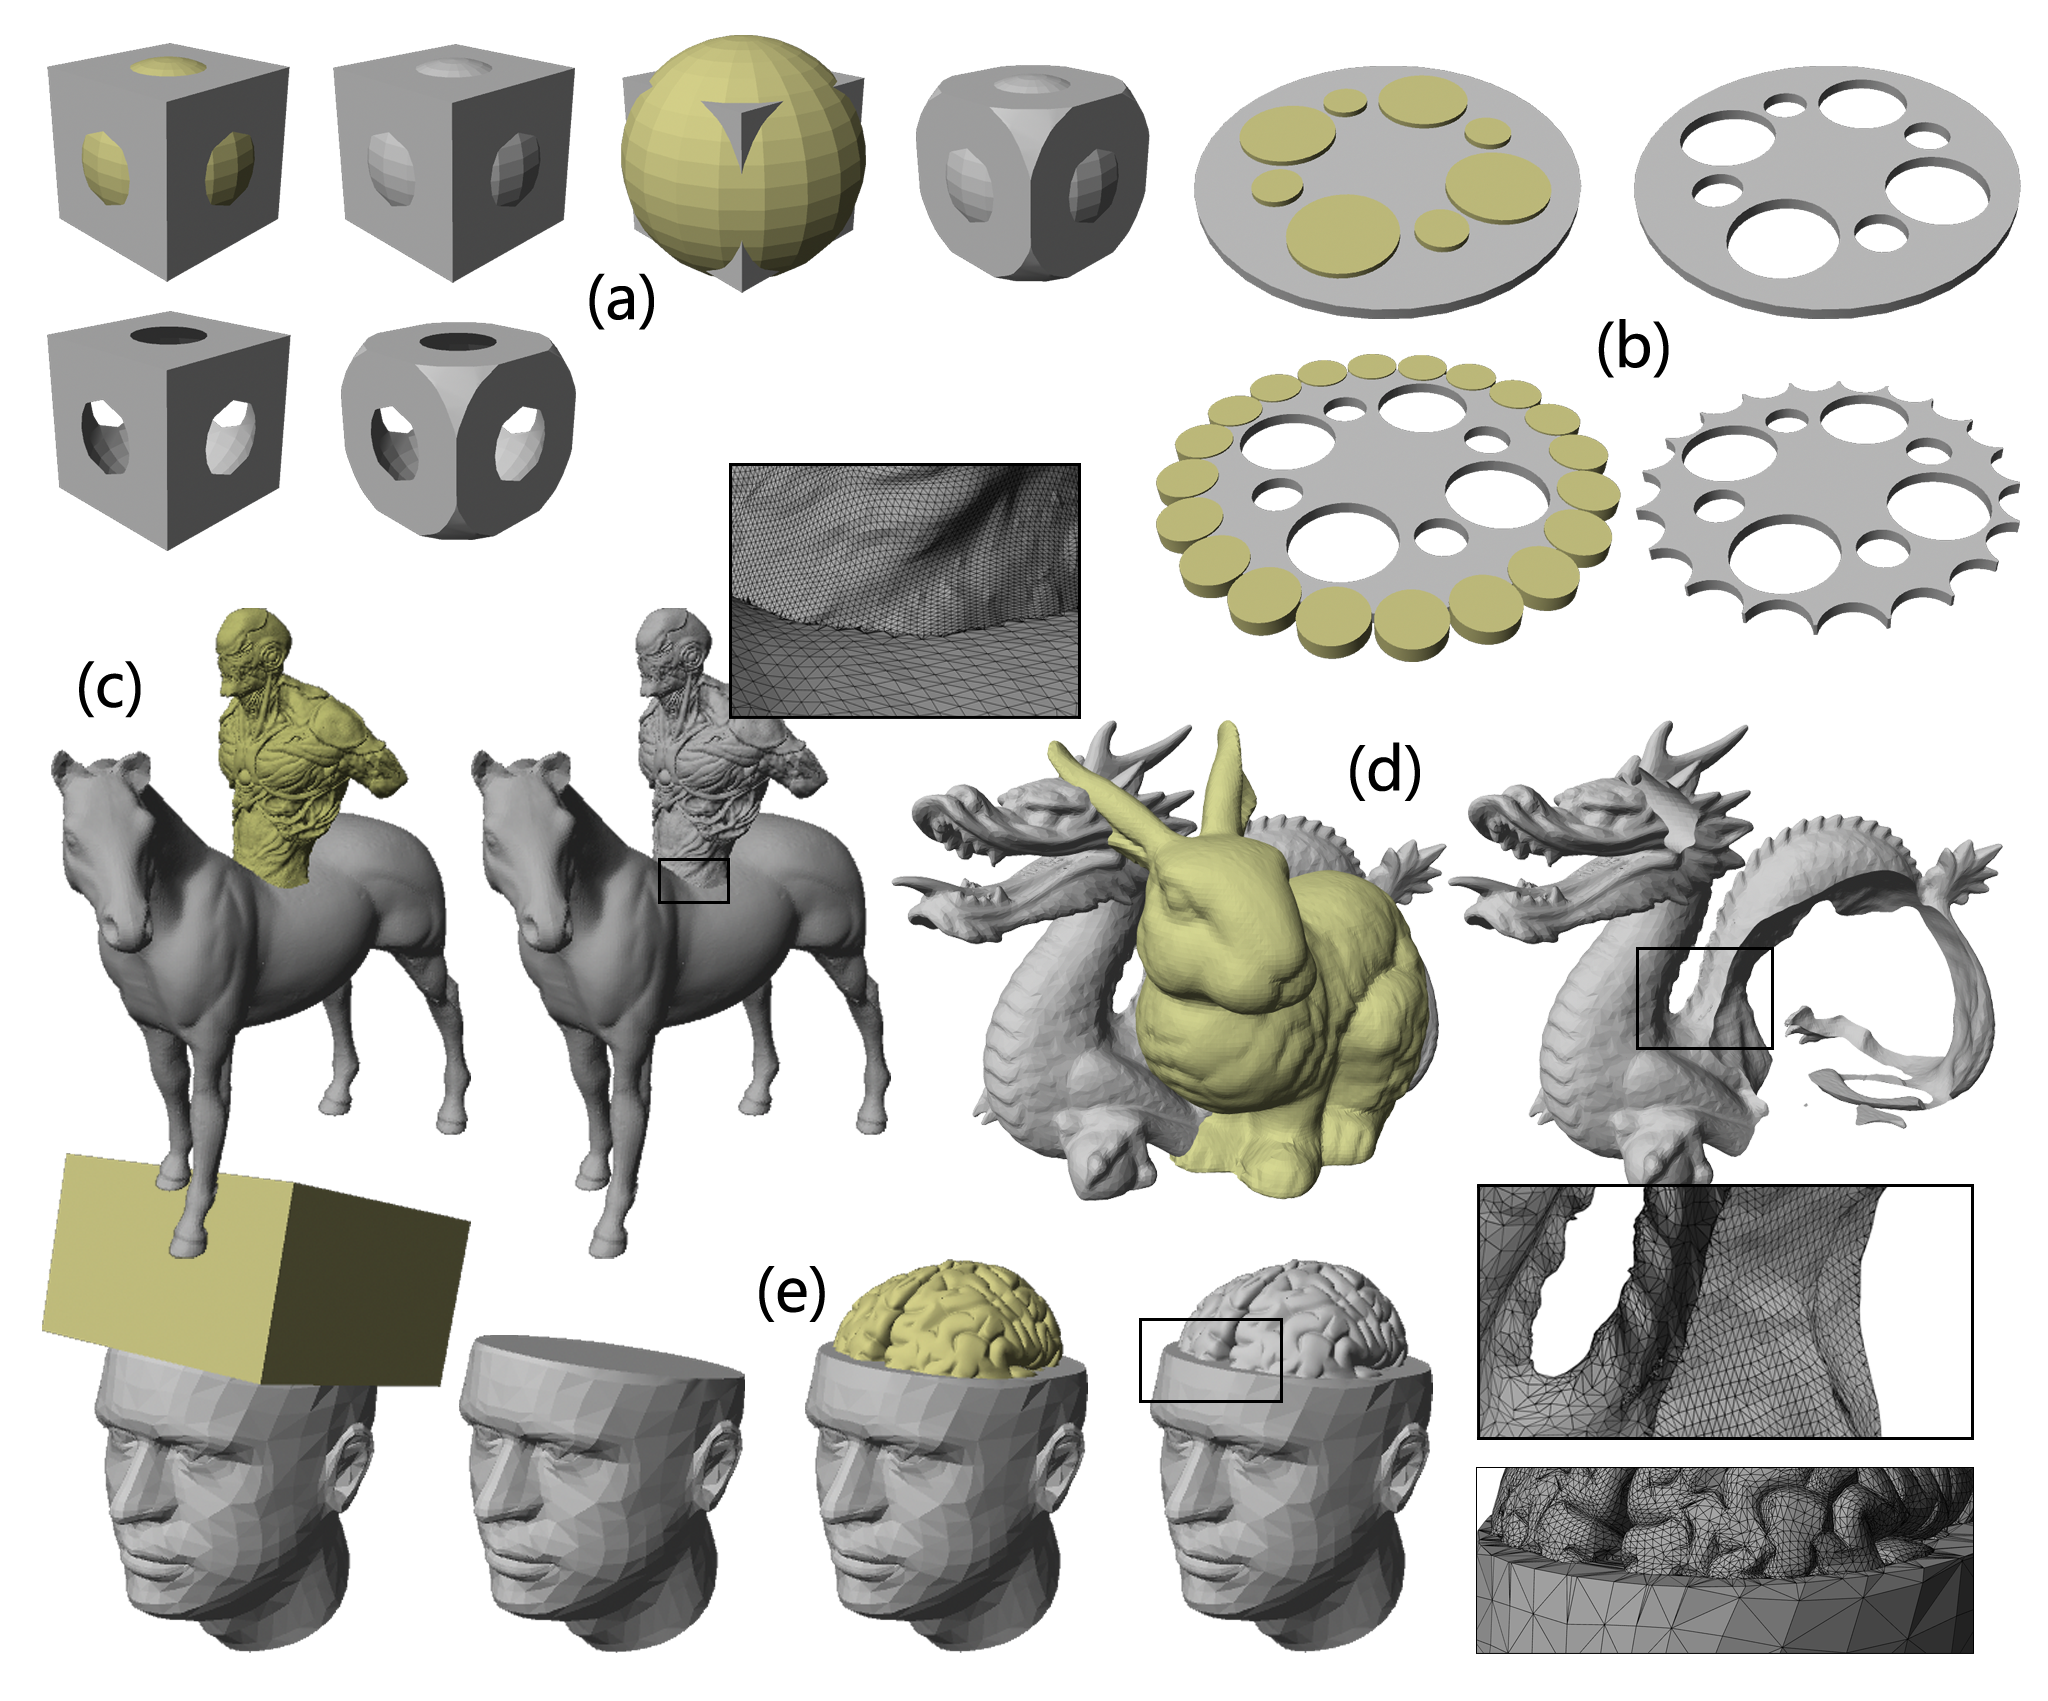
\includegraphics[width=7in]{models}
\caption{***********different models: will be replaced}
\label{fig:models}
\end{figure*}

\subsection{Implementation}
\label{sec:esubroutine}


\vspace{0.5em}
\noindent\textbf{Searching valid loops}~~~~ In \S\ref{sec:tess}, we claim a valid loops on tess-graph has to be correct with its orientation. However, since tess-graph is undirectional, it is not easy to check whether a loop orientation agrees with the face's (Fig. \ref{fig:dual}a). We observe that the graph connections lie on face edges have their unambiguous directions. Starting from these edges, we can guarantee that the loops have the right orientations. After we find a valid loop, more graph connections will have unambiguous directions because one connection can participate two valid loops at most. In such way, the correct orientation will propagate in a flood-filling way.



\vspace{0.5em} There is another problem that the tess-graph may not be a connected graph. We avoid this problem by inserting auxiliary intersections into the tess-graph to make it connected. An auxiliary intersection links the vertex of face (denoted as $\bm{v}_i$) on the outer connected component with the vertex on the inner connected component. The intersection refinement has to be performed again if the auxiliary intersections cross any other intersections. To guarantee the auxiliary intersection has a valid PBI-rep, we require the vertex from inner connected component generated by intersection between the face and an edge (denoted as $\bm{e}_j$) from other meshes---all newly introduced vertices during triangle-triangle intersection are this type. In this way, we get three vertices with exact coordinates ($\bm{v}_i$ and the two end points of $\bm{e}_j$) and can construct an exact plane where the auxiliary intersection lies.

\vspace{0.5em}
\noindent\textbf{Seed indicator generation}~~~~In \S\ref{sec:propagation}, we claim that our flood-filling starts from a seed vertex $\bm{v}_0$. While the indicator vector of the seed $\bm{\Lambda}(\bm{v}_0)$ can be generated by point-in-polyhedron test \cite{ogayar2005point} with the octree as acceleration structure \cite{frisken2002simple}, we have simpler strategies by using vertex with known indicators as the seed. We choose the vertex with the max $x$-coordinate as the seed. In this way, $\lambda_k(\bm{v}_0)$ is either $out$ ($in$, if complement is applied on mesh) or $on$. The $on$ indicators are easy to determine in most time. Though sometimes exception occur because of multi-coplanar situation, this will not happen if we carefully choose the right vertex whose neighbor faces are not coplanar.

\vspace{0.5em} The indicator vectors can propagate not only among single meshes, but can also between different meshes by the vertices and edges they share. Therefore in most time, we only need one single seed vertex for classification. However, if there are more than two connected components among meshes, we need to new seeds to propagate each component. The indicators of the second and later seeds can be computed by point-in-polyhedron tests.

\vspace{0.5em}
\noindent\textbf{Exporting to float-point number}~~~~
The vertices of final mesh in our method are represented in both P-reps and plain coordinates. While the vertices from the input meshes have there exact coordinates, the vertices newly introduced by intersection between meshes require round-off when converting to coordinates representation. Though we guarantee the correct topology in the result mesh, such round-off can still cause topology deficiencies such as self-intersections. Here we adopt Zhou et al.'s method \cite{zhou2016mesh} to solve it iteratively.

\subsection{Limitations and Future Work}

We noticed that for CSGs that contains a lot of meshes within small area (e.g., Table. \ref{tab:performance}, \emph{T1}), the performance of our method is poor. This is because in such situations, our method computes many intersections that will not appear as edges in the final mesh, which leads to unnecessary tessellation. Optimization may be explored to avoid such problem.

The input of our method is limited to regular set meshes. However, recent works claim that the piece-wise wind number (PWN) are more powerful to identify the inside and outside of meshes \cite{zhou2016mesh}.  By using PWN, the input requirements can be extended to so-called PWN meshes that allow deficiencies such as self-intersection and multi-component. It would be interesting to extend our method to PWN method in the future.


\section{Summary}

In this paper, we proposed a novel method to evaluate CSG with regular set primitives. It is able to efficiently perform unconditionally robust non-incremental boolean operations. The key idea of our approach is to embed P-reps information into B-reps. The P-reps give us the chance to strictly follow the principle of no geometry construction to avoid numerical errors. And the B-reps offer fast neighborhood query to accelerate the processing. Experiments have verified the performance of our method is competitive with state-of-the-art non-robust methods while guarantee unconditional robustness.



\appendices


%\newpage
\bibliographystyle{IEEEtran}
\bibliography{IEEEabrv,citation}


%\newpage

\begin{IEEEbiography}[{\includegraphics[width=1in,height=1.25in,clip,keepaspectratio]{rui}}]{Rui Wang}
is currently a postgraduate student at the Department of Computer Science and Technology, the Shanghai Jiao Tong University. His main research interests include real-time computer graphics and virtual reality applications.
\end{IEEEbiography}

% if you will not have a photo at all:
\begin{IEEEbiography}[{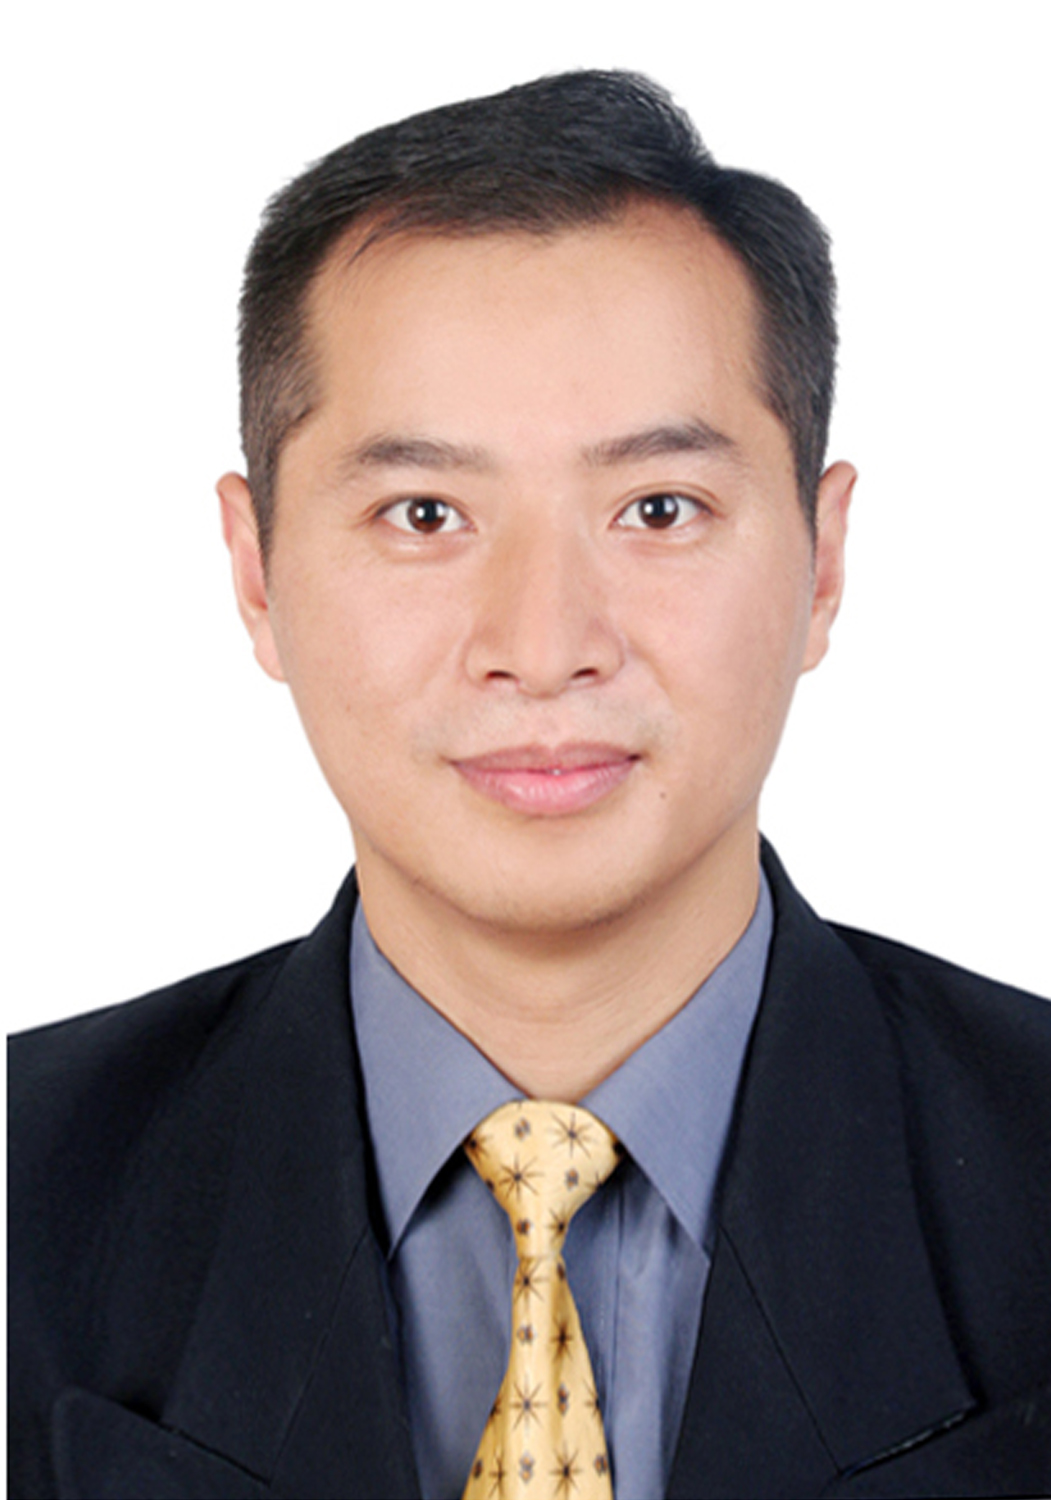
\includegraphics[width=1in,height=1.25in,clip,keepaspectratio]{xudong}}]{Xudong Jiang}
received his Master degree in Computer Science from Shanghai Jiao Tong University in 2014. He is currently working in Autodesk China Research \& Development Center. His research interest includes computer-aided geometric design and solid modeling.
\end{IEEEbiography}


\begin{IEEEbiography}[{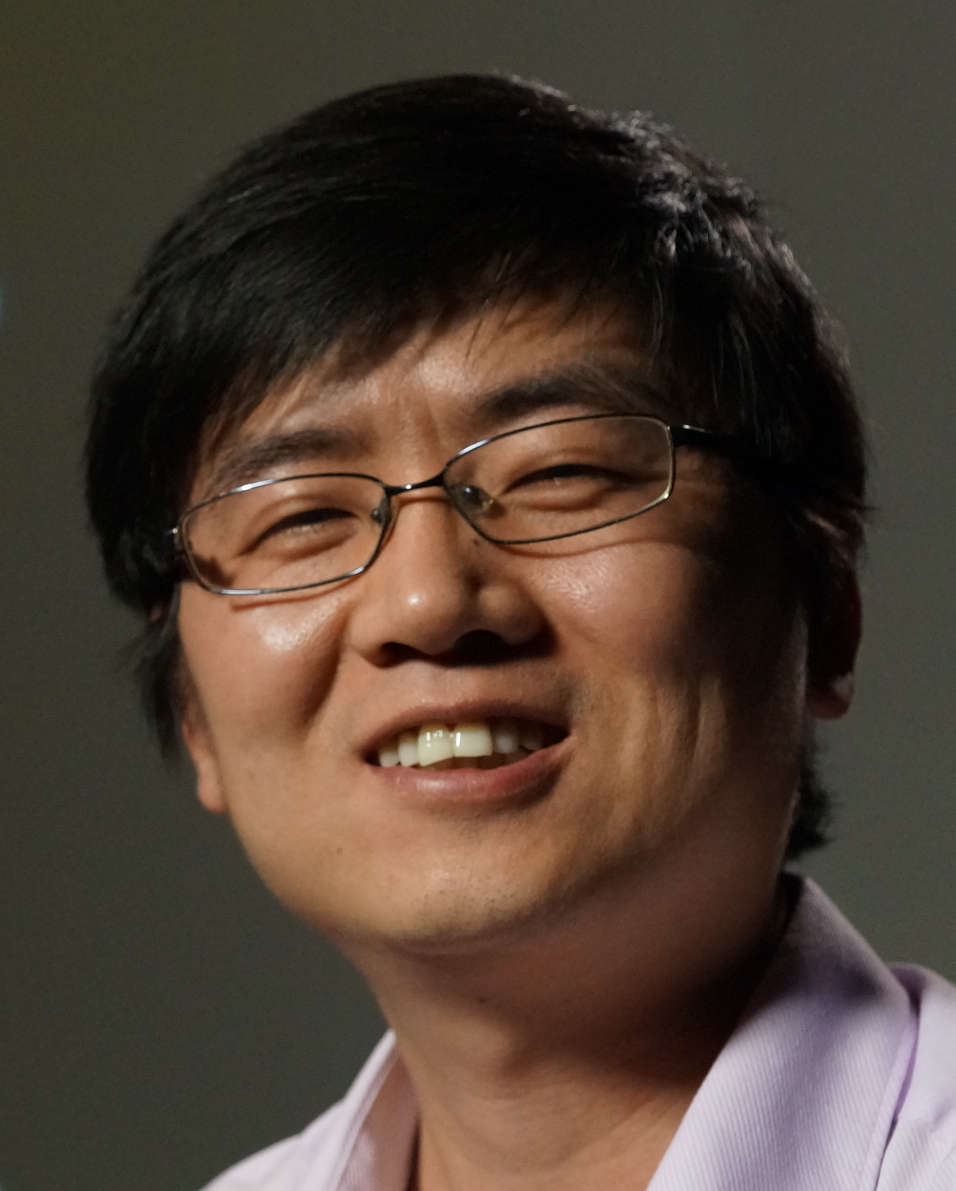
\includegraphics[width=1in,height=1.25in,clip,keepaspectratio]{hongbo}}]{Hongbu Fu}
is an Associate Professor in the School of Creative Media, City University of Hong Kong. He received the PhD degree in computer science from the Hong Kong University of Science and Technology in 2007 and the BS degree in information sciences from Peking University, China, in 2002. His primary research interests fall in the fields of computer graphics and human computer interaction. He has served as an associate editor of The Visual Computer, Computers \& Graphics, and Computer Graphics Forum.
\end{IEEEbiography}


\begin{IEEEbiography}[{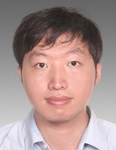
\includegraphics[width=1in,height=1.25in,clip,keepaspectratio]{sheng}}]{Bin Sheng}
received his BS degree in computer science from Huazhong University of Science and Technology in 2004, MS degree in software engineering from University of Macau in 2007, and PhD Degree in computer science from The Chinese University of Hong Kong in 2011. He is currently an associate professor in the Department of Computer Science and Engineering at Shanghai Jiao Tong University. His research interests include virtual reality, computer graphics, and image-based techniques.
\end{IEEEbiography}

\begin{IEEEbiography}[{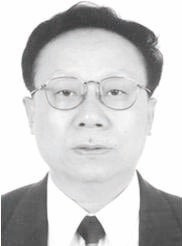
\includegraphics[width=1in,height=1.25in,clip,keepaspectratio]{wu}}]{Enhua Wu}
received the BS degree from Tsinghua University in 1970, and the PhD degree from the University of Manchester (UK) in 1984. He is currently a research professor at the Institute of Software, Chinese Academy of Sciences, and Fellow of China Computer Federation. He has also been teaching at the University of Macau since 1997, where he is currently an Emeritus Professor. His research interests include realistic image synthesis, virtual reality, and scientific visualization. He has served as an associate editor of The Visual Computer, Computer Animation and Virtual Worlds.
\end{IEEEbiography}





\end{document}


